\documentclass[type=doctor,pifootnote]{thuthesis}
% 选项:
%   type=[bachelor|master|doctor|postdoctor], % 必选
%   secret,                                   % 可选
%   pifootnote,                               % 可选(建议打开)
%   openany|openright,                        % 可选,基本不用
%   arial,                                    % 可选,基本不用
%   arialtoc,                                 % 可选,基本不用
%   arialtitle                                % 可选,基本不用

% 所有其它可能用到的包都统一放到这里了,可以根据自己的实际添加或者删除。
\usepackage{thuthesis}
\usepackage{enumitem}
\usepackage{minted}
\usepackage{amsmath}
\usepackage{cases}
% 定义所有的图片文件在 figures 子目录下

%% 使用语法高亮包
\usepackage{./template/syntax}
% 可以在这里修改配置文件中的定义。导言区可以使用中文。
% \def\myname{薛瑞尼}

% 定义\fillinblank命令,用下划线填充指定的空间。
\newcommand{\fillinblank}[2]{
	\CJKunderline{\makebox[#1]{#2}}
}

%自定义内容,包括项目组名称、月总结的年月等
\def\csriversion{v1.0}
\def\csriorg{四川大学网络空间安全研究院}
\def\csriteam{大数据平台项目组}
\def\csristartdate{2017年04月17号}
\def\csriauthor{吴天雄}
\def\csricommentor{}
\def\csricommentdate{}
%d对minted进行设置
\renewcommand{\theFancyVerbLine}{\sffamily
	\textcolor[rgb]{0.5,0.5,1.0}{\scriptsize
		\oldstylenums{\arabic{FancyVerbLine}}}}


\setminted{
	mathescape,
	linenos,
	numbersep=2pt,
	%tabsize=2,
	%frame=lines,
	framesep=2mm}
\usemintedstyle{xcode}

\begin{document}

%%% 封面部分
\frontmatter
\begin{titlepage}
\begin{center}
	% 校名和论文类别、“四川大学”字样
	{
		\ \\[-1cm]
		
\includegraphics[width=16cm]{figures/csri-name.jpg}\\[3.5cm]
		{\makebox[0.8\textwidth][c]{\zihao{1}\heiti 2017年1-3月份工作总结}}
	}
	\\[3.5cm]
	% 培养单位,指导教师,专业等信息
	{
		\zihao{-3}\kaishu
		\begin{tabular}{cc}
			{\makebox[3.2cm][s]{\textbf{版本号:}}} &\fillinblank{6.2cm}{\texttt{\csriversion}}
			\\[0.8cm]
			{\makebox[3.2cm][s]{\textbf{项目组:}}} &\fillinblank{6.2cm}{\textbf{\csriteam}}
			\\[0.8cm]
			{\makebox[3.2cm][s]{\textbf{文档作者:}}} &\fillinblank{6.2cm}{\textbf{\csriauthor}}\\[0.8cm]
			{\makebox[3.2cm][s]{\textbf{撰写日期:}}} &\fillinblank{6.2cm}{\textbf{\csristartdate}}
			\\[0.8cm]
			{\makebox[3.2cm][s]{\textbf{评审负责人:}}} &\fillinblank{6.2cm}{\textbf{\csricommentor}}
			\\[0.8cm]
			{\makebox[3.2cm][s]{\textbf{评审日期:}}} &\fillinblank{6.2cm}{\textbf{\csricommentdate}}
		\end{tabular}
	}\\[4cm]
	{\makebox[0.6\textwidth][s]{\zihao{-3}\heiti \csriorg }}
	
\end{center}
\end{titlepage}
\thispagestyle{empty}




%% 目录
\tableofcontents
%% 符号对照表
%\begin{denotation}[3cm]
\item[HPC] 高性能计算 (High Performance Computing)
\item[cluster] 集群
\item[Itanium] 安腾
\item[SMP] 对称多处理
\item[API] 应用程序编程接口
\item[PI] 聚酰亚胺
\item[MPI] 聚酰亚胺模型化合物,N-苯基邻苯酰亚胺
\item[PBI] 聚苯并咪唑
\item[MPBI] 聚苯并咪唑模型化合物,N-苯基苯并咪唑
\item[PY] 聚吡咙
\item[PMDA-BDA]	均苯四酸二酐与联苯四胺合成的聚吡咙薄膜
\item[$\Delta G$] 活化自由能 (Activation Free Energy)
\item[$\chi$] 传输系数 (Transmission Coefficient)
\item[$E$] 能量
\item[$m$] 质量
\item[$c$] 光速
\item[$P$] 概率
\item[$T$] 时间
\item[$v$] 速度
\item[劝学] 君子曰:学不可以已。青,取之于蓝,而青于蓝;冰,水为之,而寒于水。木
  直中绳。輮以为轮,其曲中规。虽有槁暴,不复挺者,輮使之然也。故木受绳则直,金就
  砺则利,君子博学而日参省乎己,则知明而行无过矣。吾尝终日而思矣,不如须臾之所学
  也;吾尝跂而望矣,不如登高之博见也。登高而招,臂非加长也,而见者远;顺风而呼,
  声非加疾也,而闻者彰。假舆马者,非利足也,而致千里;假舟楫者,非能水也,而绝江
  河,君子生非异也,善假于物也。积土成山,风雨兴焉;积水成渊,蛟龙生焉;积善成德,
  而神明自得,圣心备焉。故不积跬步,无以至千里;不积小流,无以成江海。骐骥一跃,
  不能十步;驽马十驾,功在不舍。锲而舍之,朽木不折;锲而不舍,金石可镂。蚓无爪牙
  之利,筋骨之强,上食埃土,下饮黄泉,用心一也。蟹六跪而二螯,非蛇鳝之穴无可寄托
  者,用心躁也。—— 荀况
\end{denotation}



%%% 正文部分
\mainmatter

%\chapter{带 English 的标题}
\label{cha:intro}

这是 \thuthesis{} 的示例文档,基本上覆盖了模板中所有格式的设置。建议大家在使用模
板之前,除了阅读《\thuthesis{}用户手册》,这个示例文档也最好能看一看。

小老鼠偷吃热凉粉;短长虫环绕矮高粱\footnote{韩愈(768-824),字退之,河南河阳(
  今河南孟县)人,自称郡望昌黎,世称韩昌黎。幼孤贫刻苦好学,德宗贞元八年进士。曾
  任监察御史,因上疏请免关中赋役,贬为阳山县令。后随宰相裴度平定淮西迁刑部侍郎,
  又因上表谏迎佛骨,贬潮州刺史。做过吏部侍郎,死谥文公,故世称韩吏部、韩文公。是
  唐代古文运动领袖,与柳宗元合称韩柳。诗力求险怪新奇,雄浑重气势。}。


\section{封面相关}
封面的例子请参看 cover.tex。主要符号表参看 denation.tex,附录和个人简历分别参看 appendix01.tex
和 resume.tex。里面的命令都很只管,一看即会\footnote{你说还是看不懂?怎么会呢?}。

\section{字体命令}
\label{sec:first}

苏轼(1037-1101),北宋文学家、书画家。字子瞻,号东坡居士,眉州眉山(今属四川)人
。苏洵子。嘉佑进士。神宗时曾任祠部员外郎,因反对王安石新法而求外职,任杭州通判,
知密州、徐州、湖州。后以作诗“谤讪朝廷”罪贬黄州。哲宗时任翰林学士,曾出知杭州、
颖州等,官至礼部尚书。后又贬谪惠州、儋州。北还后第二年病死常州。南宋时追谥文忠。
与父洵弟辙,合称“三苏”。在政治上属于旧党,但也有改革弊政的要求。其文汪洋恣肆,
明白畅达,为“唐宋八大家”之一。  其诗清新豪健,善用夸张比喻,在艺术表现方面独具
风格。少数诗篇也能反映民间疾苦,指责统治者的奢侈骄纵。词开豪放一派,对后代很有影
响。《念奴娇·赤壁怀古》、《水调歌头·丙辰中秋》传诵甚广。

{\kaishu 坡仙擅长行书、楷书,取法李邕、徐浩、颜真卿、杨凝式,而能自创新意。用笔丰腴
  跌宕,有天真烂漫之趣。与蔡襄、黄庭坚、米芾并称“宋四家”。能画竹,学文同,也喜
  作枯木怪石。论画主张“神似”,认为“论画以形似,见与儿童邻”;高度评价“诗中有
  画,画中有诗”的艺术造诣。诗文有《东坡七集》等。存世书迹有《答谢民师论文帖》、
  《祭黄几道文》、《前赤壁赋》、《黄州寒食诗帖》等。  画迹有《枯木怪石图》、《
  竹石图》等。}

{\fangsong 易与天地准,故能弥纶天地之道。仰以观於天文,俯以察於地理,是故知幽明之故。原
  始反终,故知死生之说。精气为物,游魂为变,是故知鬼神之情状。与天地相似,故不违。
  知周乎万物,而道济天下,故不过。旁行而不流,乐天知命,故不忧。安土敦乎仁,故
  能爱。范围天地之化而不过,曲成万物而不遗,通乎昼夜之道而知,故神无方而易无体。}

% 非本科生一般用不到幼圆与隶书字体。需要的同学请查看 ctex 文档。
{\ifcsname youyuan\endcsname\youyuan\else[无 \cs{youyuan} 字体。]\fi 有天地,然后
  万物生焉。盈天地之间者,唯万物,故受之以屯;屯者盈也,屯者物之始生也。物生必蒙,
  故受之以蒙;蒙者蒙也,物之穉也。物穉不可不养也,故受之以需;需者饮食之道也。饮
  食必有讼,故受之以讼。讼必有众起,故受之以师;师者众也。众必有所比,故受之以比;
  比者比也。比必有所畜也,故受之以小畜。物畜然后有礼,故受之以履。}

{\heiti 履而泰,然后安,故受之以泰;泰者通也。物不可以终通,故受之以否。物不可以终
  否,故受之以同人。与人同者,物必归焉,故受之以大有。有大者不可以盈,故受之以谦。
  有大而能谦,必豫,故受之以豫。豫必有随,故受之以随。以喜随人者,必有事,故受
  之以蛊;蛊者事也。}

{\ifcsname lishu\endcsname\lishu\else[无 \cs{lishu} 字体。]\fi 有事而后可大,故受
  之以临;临者大也。物大然后可观,故受之以观。可观而后有所合,故受之以噬嗑;嗑者
  合也。物不可以苟合而已,故受之以贲;贲者饰也。致饰然后亨,则尽矣,故受之以剥;
  剥者剥也。物不可以终尽,剥穷上反下,故受之以复。复则不妄矣,故受之以无妄。}

{\songti 有无妄然后可畜,故受之以大畜。物畜然后可养,故受之以颐;颐者养也。不养则不
  可动,故受之以大过。物不可以终过,故受之以坎;坎者陷也。陷必有所丽,故受之以
  离;离者丽也。}

\section{表格样本}
\label{chap1:sample:table} 

\subsection{基本表格}
\label{sec:basictable}

模板中关于表格的宏包有三个: \pkg{booktabs}、\pkg{array} 和
\pkg{longtabular},命令有一个 \cs{hlinewd}。三线表可以用 \pkg{booktabs}
提供的 \cs{toprule}、\cs{midrule} 和 \cs{bottomrule}。它们与
\pkg{longtable} 能很好的配合使用。如果表格比较简单的话可以直接用命令
\cs{hlinewd}\marg{width} 控制。
\begin{table}[htb]
  \centering
  \begin{minipage}[t]{0.8\linewidth} % 如果想在表格中使用脚注,minipage是个不错的办法
  \caption[模板文件]{模板文件。如果表格的标题很长,那么在表格索引中就会很不美
    观,所以要像 chapter 那样在前面用中括号写一个简短的标题。这个标题会出现在索
    引中。}
  \label{tab:template-files}
    \begin{tabularx}{\linewidth}{lX}
      \toprule[1.5pt]
      {\heiti 文件名} & {\heiti 描述} \\\midrule[1pt]
      thuthesis.ins & \LaTeX{} 安装文件,\textsc{DocStrip}\footnote{表格中的脚注} \\
      thuthesis.dtx & 所有的一切都在这里面\footnote{再来一个}。\\
      thuthesis.cls & 模板类文件。\\
      thuthesis.cfg & 模板配置文。cls 和 cfg 由前两个文件生成。\\
      thuthesis.bst    & 参考文献 BIB\TeX\ 样式文件。\\
      thuthesis.sty   & 常用的包和命令写在这里,减轻主文件的负担。\\
      \bottomrule[1.5pt]
    \end{tabularx}
  \end{minipage}
\end{table}

首先来看一个最简单的表格。表 \ref{tab:template-files} 列举了本模板主要文件及其功
能。请大家注意三线表中各条线对应的命令。这个例子还展示了如何在表格中正确使用脚注。
由于 \LaTeX{} 本身不支持在表格中使用 \cs{footnote},所以我们不得不将表格放在
小页中,而且最好将表格的宽度设置为小页的宽度,这样脚注看起来才更美观。

\subsection{复杂表格}
\label{sec:complicatedtable}

我们经常会在表格下方标注数据来源,或者对表格里面的条目进行解释。前面的脚注是一种
不错的方法,如果不喜欢脚注,可以在表格后面写注释,比如表~\ref{tab:tabexamp1}。
\begin{table}[htbp]
  \centering
  \caption{复杂表格示例 1}
  \label{tab:tabexamp1}
  \begin{minipage}[t]{0.8\textwidth} 
    \begin{tabularx}{\linewidth}{|l|X|X|X|X|}
      \hline
 \multirow{2}*{\diagbox[width=5em]{x}{y}} & \multicolumn{2}{c|}{First Half} & \multicolumn{2}{c|}{Second Half}\\\cline{2-5}
      & 1st Qtr &2nd Qtr&3rd Qtr&4th Qtr \\ \hline
      East$^{*}$ &   20.4&   27.4&   90&     20.4 \\
      West$^{**}$ &   30.6 &   38.6 &   34.6 &  31.6 \\ \hline
    \end{tabularx}\\[2pt]
    \footnotesize 注:数据来源《\thuthesis{} 使用手册》。\\
    *:东部\\
    **:西部
  \end{minipage}
\end{table}

此外,表~\ref{tab:tabexamp1} 同时还演示了另外两个功能:1)通过 \pkg{tabularx} 的
 \texttt{|X|} 扩展实现表格自动放大;2)通过命令 \cs{diagbox} 在表头部分
插入反斜线。

为了使我们的例子更接近实际情况,我会在必要的时候插入一些“无关”文字,以免太多图
表同时出现,导致排版效果不太理想。第一个出场的当然是我的最爱:风流潇洒、骏马绝尘、
健笔凌云的{\heiti 李太白}了。

李白,字太白,陇西成纪人。凉武昭王暠九世孙。或曰山东人,或曰蜀人。白少有逸才,志
气宏放,飘然有超世之心。初隐岷山,益州长史苏颋见而异之,曰:“是子天才英特,可比
相如。”天宝初,至长安,往见贺知章。知章见其文,叹曰:“子谪仙人也。”言于明皇,
召见金銮殿,奏颂一篇。帝赐食,亲为调羹,有诏供奉翰林。白犹与酒徒饮于市,帝坐沉香
亭子,意有所感,欲得白为乐章,召入,而白已醉。左右以水颒面,稍解,援笔成文,婉丽
精切。帝爱其才,数宴见。白常侍帝,醉,使高力士脱靴。力士素贵,耻之,摘其诗以激杨
贵妃。帝欲官白,妃辄沮止。白自知不为亲近所容,恳求还山。帝赐金放还。乃浪迹江湖,
终日沉饮。永王璘都督江陵,辟为僚佐。璘谋乱,兵败,白坐长流夜郎,会赦得还。族人阳
冰为当涂令,白往依之。代宗立,以左拾遗召,而白已卒。文宗时,诏以白歌诗、裴旻剑舞、
张旭草书为三绝云。集三十卷。今编诗二十五卷。\hfill —— 《全唐诗》诗人小传

浮动体的并排放置一般有两种情况:1)二者没有关系,为两个独立的浮动体;2)二者隶属
于同一个浮动体。对表格来说并排表格既可以像图~\ref{tab:parallel1}、图~\ref{tab:parallel2} 
使用小页环境,也可以如图~\ref{tab:subtable} 使用子表格来做。图的例子参见第~\ref{sec:multifig} 节。

\begin{table}[htbp]
\noindent\begin{minipage}{0.5\textwidth}
\centering
\caption{第一个并排子表格}
\label{tab:parallel1}
\begin{tabular}{p{2cm}p{2cm}}
\toprule[1.5pt]
111 & 222 \\\midrule[1pt]
222 & 333 \\\bottomrule[1.5pt]
\end{tabular}
\end{minipage}%
\begin{minipage}{0.5\textwidth}
\centering
\caption{第二个并排子表格}
\label{tab:parallel2}
\begin{tabular}{p{2cm}p{2cm}}
\toprule[1.5pt]
111 & 222 \\\midrule[1pt]
222 & 333 \\\bottomrule[1.5pt]
\end{tabular}
\end{minipage}
\end{table}

然后就是忧国忧民,诗家楷模杜工部了。杜甫,字子美,其先襄阳人,曾祖依艺为巩令,因
居巩。甫天宝初应进士,不第。后献《三大礼赋》,明皇奇之,召试文章,授京兆府兵曹参
军。安禄山陷京师,肃宗即位灵武,甫自贼中遁赴行在,拜左拾遗。以论救房琯,出为华州
司功参军。关辅饥乱,寓居同州同谷县,身自负薪采梠,餔糒不给。久之,召补京兆府功曹,
道阻不赴。严武镇成都,奏为参谋、检校工部员外郎,赐绯。武与甫世旧,待遇甚厚。乃于
成都浣花里种竹植树,枕江结庐,纵酒啸歌其中。武卒,甫无所依,乃之东蜀就高適。既至
而適卒。是岁,蜀帅相攻杀,蜀大扰。甫携家避乱荆楚,扁舟下峡,未维舟而江陵亦乱。乃
溯沿湘流,游衡山,寓居耒阳。卒年五十九。元和中,归葬偃师首阳山,元稹志其墓。天宝
间,甫与李白齐名,时称李杜。然元稹之言曰:“李白壮浪纵恣,摆去拘束,诚亦差肩子美
矣。至若铺陈终始,排比声韵,大或千言,次犹数百,词气豪迈,而风调清深,属对律切,
而脱弃凡近,则李尚不能历其藩翰,况堂奥乎。”白居易亦云:“杜诗贯穿古今,  尽工尽
善,殆过于李。”元、白之论如此。盖其出处劳佚,喜乐悲愤,好贤恶恶,一见之于诗。而
又以忠君忧国、伤时念乱为本旨。读其诗可以知其世,故当时谓之“诗史”。旧集诗文共六
十卷,今编诗十九卷。

\begin{table}[htbp]
\centering
\caption{并排子表格}
\label{tab:subtable}
\subcaptionbox{第一个子表格}
{
\begin{tabular}{p{2cm}p{2cm}}
\toprule[1.5pt]
111 & 222 \\\midrule[1pt]
222 & 333 \\\bottomrule[1.5pt]
\end{tabular}
}
\hskip2cm
\subcaptionbox{第二个子表格}
{
\begin{tabular}{p{2cm}p{2cm}}
\toprule[1.5pt]
111 & 222 \\\midrule[1pt]
222 & 333 \\\bottomrule[1.5pt]
\end{tabular}
}
\end{table}

不可否认 \LaTeX{} 的表格功能没有想象中的那么强大,不过只要足够认真,足够细致,
同样可以排出来非常复杂非常漂亮的表格。请参看表~\ref{tab:tabexamp2}。
\begin{table}[htbp]
  \centering\dawu[1.3]
  \caption{复杂表格示例 2}
  \label{tab:tabexamp2}
  \begin{tabular}[c]{|m{1.5cm}|c|c|c|c|c|c|}\hline
    \multicolumn{2}{|c|}{Network Topology} & \# of nodes & 
    \multicolumn{3}{c|}{\# of clients} & Server \\\hline
    GT-ITM & Waxman Transit-Stub & 600 &
    \multirow{2}{2em}{2\%}& 
    \multirow{2}{2em}{10\%}& 
    \multirow{2}{2em}{50\%}& 
    \multirow{2}{1.2in}{Max. Connectivity}\\\cline{1-3}
    \multicolumn{2}{|c|}{Inet-2.1} & 6000 & & & &\\\hline
    \multirow{2}{1.5cm}{Xue} & Rui  & Ni &\multicolumn{4}{c|}{\multirow{2}*{\thuthesis}}\\\cline{2-3}
    & \multicolumn{2}{c|}{ABCDEF} &\multicolumn{4}{c|}{} \\\hline
\end{tabular}
\end{table}

最后就是清新飘逸、文约意赅、空谷绝响的王大侠了。王维,字摩诘,河东人。工书画,与
弟缙俱有俊才。开元九年,进士擢第,调太乐丞。坐累为济州司仓参军,历右拾遗、监察御
史、左补阙、库部郎中,拜吏部郎中。天宝末,为给事中。安禄山陷两都,维为贼所得,服
药阳喑,拘于菩提寺。禄山宴凝碧池,维潜赋诗悲悼,闻于行在。贼平,陷贼官三等定罪,
特原之,责授太子中允,迁中庶子、中书舍人。复拜给事中,转尚书右丞。维以诗名盛于开
元、天宝间,宁薛诸王驸马豪贵之门,无不拂席迎之。得宋之问辋川别墅,山水绝胜,与道
友裴迪,浮舟往来,弹琴赋诗,啸咏终日。笃于奉佛,晚年长斋禅诵。一日,忽索笔作书
数纸,别弟缙及平生亲故,舍笔而卒。赠秘书监。宝应中,代宗问缙:“朕常于诸王坐闻维
乐章,今存几何?”缙集诗六卷,文四卷,表上之。敕答云,卿伯氏位列先朝,名高希代。
抗行周雅,长揖楚辞。诗家者流,时论归美。克成编录,叹息良深。殷璠谓维诗词秀调雅,
意新理惬。在泉成珠,著壁成绘。苏轼亦云:“维诗中有画,画中有诗也。”今编诗四卷。

要想用好论文模板还是得提前学习一些 \TeX/\LaTeX{}的相关知识,具备一些基本能力,掌
握一些常见技巧,否则一旦遇到问题还真是比较麻烦。我们见过很多这样的同学,一直以来
都是使用 Word 等字处理工具,以为 \LaTeX{}模板的用法也应该类似,所以就沿袭同样的思
路来对待这种所见非所得的排版工具,结果被折腾的焦头烂额,疲惫不堪。

如果您要排版的表格长度超过一页,那么推荐使用 \pkg{longtable} 或者 \pkg{supertabular}
宏包,模板对 \pkg{longtable} 进行了相应的设置,所以用起来可能简单一些。
表~\ref{tab:performance} 就是 \pkg{longtable} 的简单示例。
\begin{longtable}[c]{c*{6}{r}}
\caption{实验数据}\label{tab:performance}\\
\toprule[1.5pt]
 测试程序 & \multicolumn{1}{c}{正常运行} & \multicolumn{1}{c}{同步} & \multicolumn{1}{c}{检查点} & \multicolumn{1}{c}{卷回恢复}
& \multicolumn{1}{c}{进程迁移} & \multicolumn{1}{c}{检查点} \\
& \multicolumn{1}{c}{时间 (s)}& \multicolumn{1}{c}{时间 (s)}&
\multicolumn{1}{c}{时间 (s)}& \multicolumn{1}{c}{时间 (s)}& \multicolumn{1}{c}{
  时间 (s)}&  文件(KB)\\\midrule[1pt]
\endfirsthead
\multicolumn{7}{c}{续表~\thetable\hskip1em 实验数据}\\
\toprule[1.5pt]
 测试程序 & \multicolumn{1}{c}{正常运行} & \multicolumn{1}{c}{同步} & \multicolumn{1}{c}{检查点} & \multicolumn{1}{c}{卷回恢复}
& \multicolumn{1}{c}{进程迁移} & \multicolumn{1}{c}{检查点} \\
& \multicolumn{1}{c}{时间 (s)}& \multicolumn{1}{c}{时间 (s)}&
\multicolumn{1}{c}{时间 (s)}& \multicolumn{1}{c}{时间 (s)}& \multicolumn{1}{c}{
  时间 (s)}&  文件(KB)\\\midrule[1pt]
\endhead
\hline
\multicolumn{7}{r}{续下页}
\endfoot
\endlastfoot
CG.A.2 & 23.05 & 0.002 & 0.116 & 0.035 & 0.589 & 32491 \\
CG.A.4 & 15.06 & 0.003 & 0.067 & 0.021 & 0.351 & 18211 \\
CG.A.8 & 13.38 & 0.004 & 0.072 & 0.023 & 0.210 & 9890 \\
CG.B.2 & 867.45 & 0.002 & 0.864 & 0.232 & 3.256 & 228562 \\
CG.B.4 & 501.61 & 0.003 & 0.438 & 0.136 & 2.075 & 123862 \\
CG.B.8 & 384.65 & 0.004 & 0.457 & 0.108 & 1.235 & 63777 \\
MG.A.2 & 112.27 & 0.002 & 0.846 & 0.237 & 3.930 & 236473 \\
MG.A.4 & 59.84 & 0.003 & 0.442 & 0.128 & 2.070 & 123875 \\
MG.A.8 & 31.38 & 0.003 & 0.476 & 0.114 & 1.041 & 60627 \\
MG.B.2 & 526.28 & 0.002 & 0.821 & 0.238 & 4.176 & 236635 \\
MG.B.4 & 280.11 & 0.003 & 0.432 & 0.130 & 1.706 & 123793 \\
MG.B.8 & 148.29 & 0.003 & 0.442 & 0.116 & 0.893 & 60600 \\
LU.A.2 & 2116.54 & 0.002 & 0.110 & 0.030 & 0.532 & 28754 \\
LU.A.4 & 1102.50 & 0.002 & 0.069 & 0.017 & 0.255 & 14915 \\
LU.A.8 & 574.47 & 0.003 & 0.067 & 0.016 & 0.192 & 8655 \\
LU.B.2 & 9712.87 & 0.002 & 0.357 & 0.104 & 1.734 & 101975 \\
LU.B.4 & 4757.80 & 0.003 & 0.190 & 0.056 & 0.808 & 53522 \\
LU.B.8 & 2444.05 & 0.004 & 0.222 & 0.057 & 0.548 & 30134 \\
EP.A.2 & 123.81 & 0.002 & 0.010 & 0.003 & 0.074 & 1834 \\
EP.A.4 & 61.92 & 0.003 & 0.011 & 0.004 & 0.073 & 1743 \\
EP.A.8 & 31.06 & 0.004 & 0.017 & 0.005 & 0.073 & 1661 \\
EP.B.2 & 495.49 & 0.001 & 0.009 & 0.003 & 0.196 & 2011 \\
EP.B.4 & 247.69 & 0.002 & 0.012 & 0.004 & 0.122 & 1663 \\
EP.B.8 & 126.74 & 0.003 & 0.017 & 0.005 & 0.083 & 1656 \\
\bottomrule[1.5pt]
\end{longtable}

\subsection{其它}
\label{sec:tableother}
如果不想让某个表格或者图片出现在索引里面,请使用命令 \cs{caption*}。
这个命令不会给表格编号,也就是出来的只有标题文字而没有“表~XX”,“图~XX”,否则
索引里面序号不连续就显得不伦不类,这也是 \LaTeX{} 里星号命令默认的规则。

有这种需求的多是本科同学的英文资料翻译部分,如果觉得附录中英文原文中的表格和图
片显示成“表”和“图”不协调的话,一个很好的办法就是用 \cs{caption*},参数
随便自己写,比如不守规矩的表~1.111 和图~1.111 能满足这种特殊需要(可以参看附录部
分)。
\begin{table}[ht]
  \begin{minipage}{0.4\linewidth}
    \centering
    \caption*{表~1.111\quad 这是一个手动编号,不出现在索引中的表格。}
    \label{tab:badtabular}
      \framebox(150,50)[c]{\thuthesis}
  \end{minipage}%
  \hfill%
  \begin{minipage}{0.4\linewidth}
    \centering
    \caption*{Figure~1.111\quad 这是一个手动编号,不出现在索引中的图。}
    \label{tab:badfigure}
    \framebox(150,50)[c]{薛瑞尼}
  \end{minipage}
\end{table}

如果的确想让它编号,但又不想让它出现在索引中的话,目前模板上不支持。

最后,虽然大家不一定会独立使用小页,但是关于小页中的脚注还是有必要提一下。请看下
面的例子。

\begin{minipage}[t]{\linewidth-2\parindent}
  柳宗元,字子厚(773-819),河东(今永济县)人\footnote{山西永济水饺。},是唐代
  杰出的文学家,哲学家,同时也是一位政治改革家。与韩愈共同倡导唐代古文运动,并称
  韩柳\footnote{唐宋八大家之首二位。}。
\end{minipage}

唐朝安史之乱后,宦官专权,藩镇割据,土地兼并日渐严重,社会生产破坏严重,民不聊生。柳宗
元对这种社会现实极为不满,他积极参加了王叔文领导的“永济革新”,并成为这一
运动的中坚人物。他们革除弊政,打击权奸,触犯了宦官和官僚贵族利益,在他们的联合反
扑下,改革失败了,柳宗元被贬为永州司马。

\section{定理环境}
\label{sec:theorem}

给大家演示一下各种和证明有关的环境:

\begin{assumption}
待月西厢下,迎风户半开;隔墙花影动,疑是玉人来。
\begin{eqnarray}
  \label{eq:eqnxmp}
  c & = & a^2 - b^2\\
    & = & (a+b)(a-b)
\end{eqnarray}
\end{assumption}

千辛万苦,历尽艰难,得有今日。然相从数千里,未曾哀戚。今将渡江,方图百年欢笑,如
何反起悲伤?(引自《杜十娘怒沉百宝箱》)

\begin{definition}
子曰:「道千乘之国,敬事而信,节用而爱人,使民以时。」
\end{definition}

千古第一定义!问世间、情为何物,只教生死相许?天南地北双飞客,老翅几回寒暑。欢乐趣,离别苦,就中更有痴儿女。
君应有语,渺万里层云,千山暮雪,只影向谁去?

横汾路,寂寞当年箫鼓,荒烟依旧平楚。招魂楚些何嗟及,山鬼暗谛风雨。天也妒,未信与,莺儿燕子俱黄土。
千秋万古,为留待骚人,狂歌痛饮,来访雁丘处。

\begin{proposition}
 曾子曰:「吾日三省吾身 —— 为人谋而不忠乎?与朋友交而不信乎?传不习乎?」
\end{proposition}

多么凄美的命题啊!其日牛马嘶,新妇入青庐,奄奄黄昏后,寂寂人定初,我命绝今日,
魂去尸长留,揽裙脱丝履,举身赴清池,府吏闻此事,心知长别离,徘徊庭树下,自挂东南
枝。

\begin{remark}
天不言自高,水不言自流。
\begin{gather*}
\begin{split} 
\varphi(x,z)
&=z-\gamma_{10}x-\gamma_{mn}x^mz^n\\
&=z-Mr^{-1}x-Mr^{-(m+n)}x^mz^n
\end{split}\\[6pt]
\begin{align} \zeta^0&=(\xi^0)^2,\\
\zeta^1 &=\xi^0\xi^1,\\
\zeta^2 &=(\xi^1)^2,
\end{align}
\end{gather*}
\end{remark}

天尊地卑,乾坤定矣。卑高以陈,贵贱位矣。 动静有常,刚柔断矣。方以类聚,物以群分,
吉凶生矣。在天成象,在地成形,变化见矣。鼓之以雷霆,润之以风雨,日月运行,一寒一
暑,乾道成男,坤道成女。乾知大始,坤作成物。乾以易知,坤以简能。易则易知,简则易
从。易知则有亲,易从则有功。有亲则可久,有功则可大。可久则贤人之德,可大则贤人之
业。易简,而天下矣之理矣;天下之理得,而成位乎其中矣。

\begin{axiom}
两点间直线段距离最短。  
\begin{align}
x&\equiv y+1\pmod{m^2}\\
x&\equiv y+1\mod{m^2}\\
x&\equiv y+1\pod{m^2}
\end{align}
\end{axiom}

《彖曰》:大哉乾元,万物资始,乃统天。云行雨施,品物流形。大明始终,六位时成,时
乘六龙以御天。乾道变化,各正性命,保合大和,乃利贞。首出庶物,万国咸宁。

《象曰》:天行健,君子以自强不息。潜龙勿用,阳在下也。见龙再田,德施普也。终日乾
乾,反复道也。或跃在渊,进无咎也。飞龙在天,大人造也。亢龙有悔,盈不可久也。用九,
天德不可为首也。   

\begin{lemma}
《猫和老鼠》是我最爱看的动画片。
\begin{multline*}%\tag*{[a]} % 这个不出现在索引中
\int_a^b\biggl\{\int_a^b[f(x)^2g(y)^2+f(y)^2g(x)^2]
 -2f(x)g(x)f(y)g(y)\,dx\biggr\}\,dy \\
 =\int_a^b\biggl\{g(y)^2\int_a^bf^2+f(y)^2
  \int_a^b g^2-2f(y)g(y)\int_a^b fg\biggr\}\,dy
\end{multline*}
\end{lemma}

行行重行行,与君生别离。相去万余里,各在天一涯。道路阻且长,会面安可知。胡马依北
风,越鸟巢南枝。相去日已远,衣带日已缓。浮云蔽白日,游子不顾返。思君令人老,岁月
忽已晚。  弃捐勿复道,努力加餐饭。

\begin{theorem}\label{the:theorem1}
犯我强汉者,虽远必诛\hfill —— 陈汤(汉)
\end{theorem}
\begin{subequations}
\begin{align}
y & = 1 \\
y & = 0
\end{align}
\end{subequations}
道可道,非常道。名可名,非常名。无名天地之始;有名万物之母。故常无,欲以观其妙;
常有,欲以观其徼。此两者,同出而异名,同谓之玄。玄之又玄,众妙之门。上善若水。水
善利万物而不争,处众人之所恶,故几于道。曲则全,枉则直,洼则盈,敝则新,少则多,
多则惑。人法地,地法天,天法道,道法自然。知人者智,自知者明。胜人者有力,自胜
者强。知足者富。强行者有志。不失其所者久。死而不亡者寿。

\begin{proof}
燕赵古称多感慨悲歌之士。董生举进士,连不得志于有司,怀抱利器,郁郁适兹土,吾
知其必有合也。董生勉乎哉?

夫以子之不遇时,苟慕义强仁者,皆爱惜焉,矧燕、赵之士出乎其性者哉!然吾尝闻
风俗与化移易,吾恶知其今不异于古所云邪?聊以吾子之行卜之也。董生勉乎哉?

吾因子有所感矣。为我吊望诸君之墓,而观于其市,复有昔时屠狗者乎?为我谢
曰:“明天子在上,可以出而仕矣!” \hfill —— 韩愈《送董邵南序》
\end{proof}

\begin{corollary}
  四川话配音的《猫和老鼠》是世界上最好看最好听最有趣的动画片。
\begin{alignat}{3}
V_i & =v_i - q_i v_j, & \qquad X_i & = x_i - q_i x_j,
 & \qquad U_i & = u_i,
 \qquad \text{for $i\ne j$;}\label{eq:B}\\
V_j & = v_j, & \qquad X_j & = x_j,
  & \qquad U_j & u_j + \sum_{i\ne j} q_i u_i.
\end{alignat}
\end{corollary}

迢迢牵牛星,皎皎河汉女。
纤纤擢素手,札札弄机杼。
终日不成章,泣涕零如雨。
河汉清且浅,相去复几许。
盈盈一水间,脉脉不得语。

\begin{example}
  大家来看这个例子。
\begin{equation}
\label{ktc}
\left\{\begin{array}{l}
\nabla f({\mbox{\boldmath $x$}}^*)-\sum\limits_{j=1}^p\lambda_j\nabla g_j({\mbox{\boldmath $x$}}^*)=0\\[0.3cm]
\lambda_jg_j({\mbox{\boldmath $x$}}^*)=0,\quad j=1,2,\cdots,p\\[0.2cm]
\lambda_j\ge 0,\quad j=1,2,\cdots,p.
\end{array}\right.
\end{equation}
\end{example}

\begin{exercise}
  清列出 Andrew S. Tanenbaum 和 W. Richard Stevens 的所有著作。
\end{exercise}

\begin{conjecture} \textit{Poincare Conjecture} If in a closed three-dimensional
  space, any closed curves can shrink to a point continuously, this space can be
  deformed to a sphere.
\end{conjecture}

\begin{problem}
 回答还是不回答,是个问题。 
\end{problem}

如何引用定理~\ref{the:theorem1} 呢?加上 \cs{label} 使用 \cs{ref} 即可。妾发
初覆额,折花门前剧。郎骑竹马来,绕床弄青梅。同居长干里,两小无嫌猜。 十四为君妇,
羞颜未尝开。低头向暗壁,千唤不一回。十五始展眉,愿同尘与灰。常存抱柱信,岂上望夫
台。 十六君远行,瞿塘滟滪堆。五月不可触,猿声天上哀。门前迟行迹,一一生绿苔。苔深
不能扫,落叶秋风早。八月蝴蝶来,双飞西园草。感此伤妾心,坐愁红颜老。

\section{参考文献}
\label{sec:bib}
当然参考文献可以直接写 \cs{bibitem},虽然费点功夫,但是好控制,各种格式可以自己随意改
写。

本模板推荐使用 BIB\TeX,样式文件为 \texttt{thuthesis.bst},基本符合学校的参考文献格
式(如专利等引用未加详细测试)。看看这个例子,关于书的~\cite{tex, companion,
  ColdSources},还有这些~\cite{Krasnogor2004e, clzs, zjsw},关于杂志
的~\cite{ELIDRISSI94, MELLINGER96, SHELL02},硕士论文~\cite{zhubajie,
  metamori2004},博士论文~\cite{shaheshang, FistSystem01},标准文
件~\cite{IEEE-1363},会议论文~\cite{DPMG,kocher99},技术报告~\cite{NPB2},电子文
献~\cite{chuban2001,oclc2000}。中文参考文献~\cite{cnarticle}应增
加 \texttt{lang=``zh''} 字段,以便进行相应处理。另外,本模板对中文文
献~\cite{cnproceed}的支持并不是十全十美,如果有不如意的地方,请手动修
改 \texttt{bbl} 文件。

有时候不想要上标,那么可以这样~\inlinecite{shaheshang},这个非常重要。

有时候一些参考文献没有纸质出处,需要标注 URL。缺省情况下,URL 不会在连字符处断行,
这可能使得用连字符代替空格的网址分行很难看。如果需要,可以将模板类文件中
\begin{verbatim}
\RequirePackage{hyperref}
\end{verbatim}
一行改为:
\begin{verbatim}
\PassOptionsToPackage{hyphens}{url}
\RequirePackage{hyperref}
\end{verbatim}
使得连字符处可以断行。更多设置可以参考 \texttt{url} 宏包文档。

\section{公式}
\label{sec:equation}
贝叶斯公式如式~(\ref{equ:chap1:bayes}),其中 $p(y|\mathbf{x})$ 为后验;
$p(\mathbf{x})$ 为先验;分母 $p(\mathbf{x})$ 为归一化因子。
\begin{equation}
\label{equ:chap1:bayes}
p(y|\mathbf{x}) = \frac{p(\mathbf{x},y)}{p(\mathbf{x})}=
\frac{p(\mathbf{x}|y)p(y)}{p(\mathbf{x})} 
\end{equation}

论文里面公式越多,\TeX{} 就越 happy。再看一个 \pkg{amsmath} 的例子:
\newcommand{\envert}[1]{\left\lvert#1\right\rvert} 
\begin{equation}\label{detK2}
\det\mathbf{K}(t=1,t_1,\dots,t_n)=\sum_{I\in\mathbf{n}}(-1)^{\envert{I}}
\prod_{i\in I}t_i\prod_{j\in I}(D_j+\lambda_jt_j)\det\mathbf{A}
^{(\lambda)}(\overline{I}|\overline{I})=0.
\end{equation} 

前面定理示例部分列举了很多公式环境,可以说把常见的情况都覆盖了,大家在写公式的时
候一定要好好看 \pkg{amsmath} 的文档,并参考模板中的用法:
\begin{multline*}%\tag{[b]} % 这个出现在索引中的
\int_a^b\biggl\{\int_a^b[f(x)^2g(y)^2+f(y)^2g(x)^2]
 -2f(x)g(x)f(y)g(y)\,dx\biggr\}\,dy \\
 =\int_a^b\biggl\{g(y)^2\int_a^bf^2+f(y)^2
  \int_a^b g^2-2f(y)g(y)\int_a^b fg\biggr\}\,dy
\end{multline*}

其实还可以看看这个多级规划:
\begin{equation}\label{bilevel}
\left\{\begin{array}{l}
\max\limits_{{\mbox{\footnotesize\boldmath $x$}}} F(x,y_1^*,y_2^*,\cdots,y_m^*)\\[0.2cm]
\mbox{subject to:}\\[0.1cm]
\qquad G(x)\le 0\\[0.1cm]
\qquad(y_1^*,y_2^*,\cdots,y_m^*)\mbox{ solves problems }(i=1,2,\cdots,m)\\[0.1cm]
\qquad\left\{\begin{array}{l}
    \max\limits_{{\mbox{\footnotesize\boldmath $y_i$}}}f_i(x,y_1,y_2,\cdots,y_m)\\[0.2cm]
    \mbox{subject to:}\\[0.1cm]
    \qquad g_i(x,y_1,y_2,\cdots,y_m)\le 0.
    \end{array}\right.
\end{array}\right.
\end{equation}
这些跟规划相关的公式都来自于刘宝碇老师《不确定规划》的课件。

%\chapter{中华人民共和国}
\label{cha:china}

\section{其它例子}
\label{sec:other}

在第~\ref{cha:intro} 章中我们学习了贝叶斯公式~(\ref{equ:chap1:bayes}),这里我们复
习一下:
\begin{equation}
\label{equ:chap2:bayes}
p(y|\mathbf{x}) = \frac{p(\mathbf{x},y)}{p(\mathbf{x})}=
\frac{p(\mathbf{x}|y)p(y)}{p(\mathbf{x})}
\end{equation}

\subsection{绘图}
\label{sec:draw}

本模板不再预先装载任何绘图包(如 \pkg{pstricks,pgf} 等),完全由用户来决定。
个人觉得 \pkg{pgf} 不错,不依赖于 Postscript。此外还有很多针对 \LaTeX{} 的
 GUI 作图工具,如 XFig(jFig), WinFig, Tpx, Ipe, Dia, Inkscape, LaTeXPiX,
jPicEdt, jaxdraw 等等。

\subsection{插图}
\label{sec:graphs}

强烈推荐《\LaTeXe\ 插图指南》!关于子图形的使用细节请参看 \pkg{subcaption} 宏包的说明文档。

\subsubsection{一个图形}
\label{sec:onefig}
一般图形都是处在浮动环境中。之所以称为浮动是指最终排版效果图形的位置不一定与源文
件中的位置对应\footnote{This is not a bug, but a feature of \LaTeX!},这也是刚使
用 \LaTeX{} 同学可能遇到的问题。如果要强制固定浮动图形的位置,请使用 \pkg{float} 宏包,
它提供了 \texttt{[H]} 参数,比如图~\ref{fig:xfig1}。
\begin{figure}[H] % use float package if you want it here
  \centering
  
\includegraphics{figures/thu-whole-logo}
  \caption{利用 Xfig 制图}
  \label{fig:xfig1}
\end{figure}

大学之道,在明明德,在亲民,在止于至善。知止而后有定;定而后能静;静而后能安;安
而后能虑;虑而后能得。物有本末,事有终始。知所先后,则近道矣。古之欲明明德于天
下者,先治其国;欲治其国者,先齐其家;欲齐其家者,先修其身;欲修其身者,先正其心;
欲正其心者,先诚其意;欲诚其意者,先致其知;致知在格物。物格而后知至;知至而后
意诚;意诚而后心正;心正而后身 修;身修而后家齐;家齐而后国治;国治而后天下
平。自天子以至于庶人,壹是皆以修身为本。其本乱而未治者 否矣。其所厚者薄,而其所
薄者厚,未之有也!

\hfill —— 《大学》


\subsubsection{多个图形}
\label{sec:multifig}

如果多个图形相互独立,并不共用一个图形计数器,那么
用 \texttt{minipage} 或者\texttt{parbox} 就可以。否则,请参看
图~\ref{fig:big1-subcaptionbox},它包含两个小图,分别是图~\ref{fig:subfig1}和
图~\ref{fig:subfig2}。推荐使用\cs{subcaptionbox},因为可以像
图~\ref{fig:big1-subcaptionbox} 那样对齐子图的标题,也可以使
用\pkg{subcaption}宏包的\cs{subcaption}(放在 minipage中,用法同\cs{caption})
或是 \pkg{subfigure} 、 \pkg{subtable}环境,像图~\ref{fig:big1-subfigure},
不要再用 \cs{subfloat}、\cs{subfigure} 和 \cs{subtable}。

\begin{figure}[h]
  \centering%
  \subcaptionbox{第一个小图形\label{fig:subfig1}}[3cm] %标题的长度,超过则会换行,如下一个小图。
    {
\includegraphics[height=3cm]{thu-fig-logo}}%
  \hspace{4em}%
  \subcaptionbox{第二个小图形,注意这个图略矮些。如果标题很长的话,它会自动换行\label{fig:subfig2}}
      {
\includegraphics[height=2cm]{thu-text-logo}}
  \caption{包含子图形的大图形(subcaptionbox示例)}
  \label{fig:big1-subcaptionbox}
\end{figure}
\begin{figure}[h]
  \centering%
  \begin{subfigure}{3cm}
    
\includegraphics[height=3cm]{thu-fig-logo}
    \caption{第一个小图形}
  \end{subfigure}%
  \hspace{4em}%
  \begin{subfigure}{0.5\textwidth}
    
\includegraphics[height=2cm]{thu-text-logo}
    \caption{第二个小图形,注意这个图略矮些。subfigure中同一行的子图在顶端对齐。}
  \end{subfigure}
  \caption{包含子图形的大图形(subfigure示例)}
  \label{fig:big1-subfigure}
\end{figure}

古之学者必有师。师者,所以传道受业解惑也。人非生而知之者,孰能无惑?惑而不从师,
其为惑也,终不解矣。生乎吾前,其闻道也固先乎吾,吾从而师之;生乎吾後,其闻道也亦
先乎吾,吾从而师之。吾师道也,夫庸知其年之先後生於吾乎!是故无贵无贱无长无少,道
之所存,师之所存也。

嗟乎!师道之不传也久矣,欲人之无惑也难矣。古之圣人,其出人也远矣,犹且从师而问焉;
今之众人,其下圣人也亦远矣,而耻学於师。是故圣益圣,愚益愚。圣人之所以为圣,愚
人之所以为愚,其皆出於此乎?爱其子,择师而教之,於其身也,则耻师焉,惑焉。彼童子
之师,授之书而习其句读者,非吾所谓传其道、解其惑者也。句读之不知,惑之不解,或师
焉,或不焉,小学而大遗,吾未见其明也。巫医、乐师、百工之人不耻相师,  士大夫之族
曰“师”曰“弟子”之云者,则群聚而笑之。问之,则曰:彼与彼年相若也,道相似也,位
卑则足羞,官盛则近谀。呜呼!师道之不复,可知矣。巫医、乐师、百工之人。吾子不齿,
今其智乃反不能及,其可怪也欤!圣人无常师。孔子师郯子、苌子、师襄、老聃。郯子之徒,
其贤不及孔子。孔子曰:“三人行,必有我师。”是故弟子不必不如师,师不必贤於弟子。
闻道有先後,术业有专攻,如是而已。

如果要把编号的两个图形并排,那么小页就非常有用了:
\begin{figure}
\begin{minipage}{0.48\textwidth}
  \centering
  
\includegraphics[height=2cm]{thu-whole-logo}
  \caption{并排第一个图}
  \label{fig:parallel1}
\end{minipage}\hfill
\begin{minipage}{0.48\textwidth}
  \centering
  
\includegraphics[height=2cm]{thu-whole-logo}
  \caption{并排第二个图}
  \label{fig:parallel2}
\end{minipage}
\end{figure}

李氏子蟠,年十七,好古文、六艺,经传皆通习之,不拘於时,学於余。余嘉其能行古
道,作师说以贻之。

\hfill —— 韩愈(唐)

\chapter{Spark应用启动过程分析}
\label{cha:run_wordcount}
\section{WordCount程序}
\label{sec:spark_wd}
阅读Spark源码以Spark集群中运行WordCount应用顺序为根据,理解出Spark应用运行的流程,从而达到阅读源码的目的。

本WordCount源码如程序\ref{lst:spark_wd}所示:

\begin{lstlisting}[
caption = {基于Spark的WordCount程序},
label={lst:spark_wd},
language = Scala
]
package org.apache.spark.examples
import org.apache.spark.{SparkConf, SparkContext}
object HelloWorld {
def main(args: Array[String]): Unit = {
    val scf = new SparkConf();
    scf.setAppName("Spark Count")
    val sc = new SparkContext(scf)
    val scfclone = sc.getConf
    val threshold = args(1).toInt
    val tokenizde = sc.textFile(args(0)).flatMap(_.split(" "))
    println("tokenizde: " + tokenizde)
    val wordCount = tokenizde.map((_, 1)).reduceByKey(_ + _)
    println("wordCount: " + wordCount)
    val filtered = wordCount.filter(_._2 >= threshold)
    val charCount = filtered.flatMap(_._1.toCharArray).map((_,1)).reduceByKey(_+_)
    println(filtered.collect().mkString(","))
  }
}
\end{lstlisting}

将输入案例input.txt放入hdfs中,已搭建好环境的Spark集群,打包好的WordCount jar包且提交到集群中的任意一台机器(本例中为master)中。

\section{提交WordCount程序}
\label{sec:submit_app}
程序提交的整个过程如图\ref{spark-submit}所示:
\begin{figure}[H] % use float package if you want it here
	\centering
	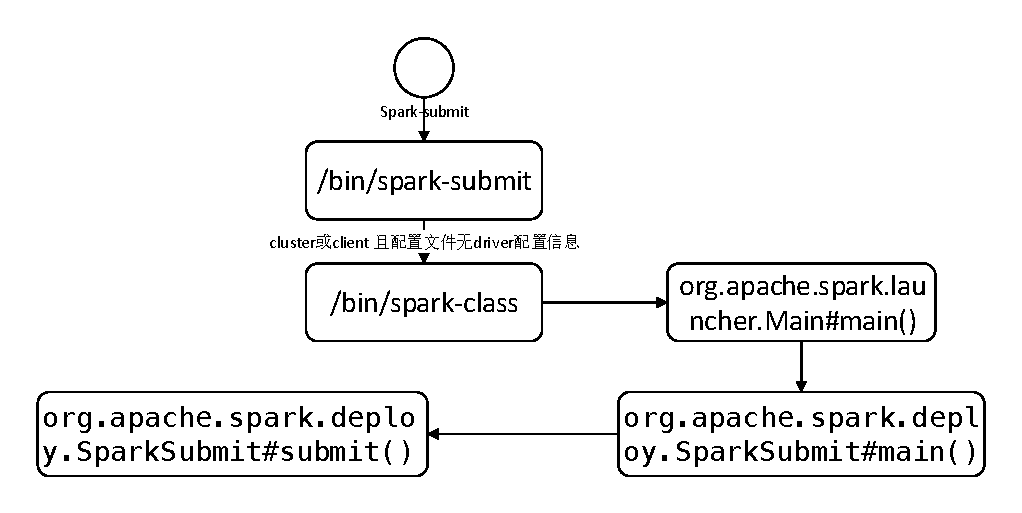
\includegraphics{figures/sparksubmit.pdf}
	\caption{spark-submit运行流程}
	\label{spark-submit}
\end{figure}

在master中运行提交命令如下:
	
\begin{cmd}
/usr/bin/spark-submit
   HelloWorld-1.0-SNAPSHOT-jar-with-dependencies.jar
   /user/inputfile.txt 2
\end{cmd}

从这条命令可以看出使用的是spark-submit shell脚本,后面三个为参数,第一个为目录下的WordCount jar包,第二个为hdfs中的输入文件,第三个为WordCount中限定输出的value临界值。
我们打开spark-submit shell脚本,脚本如所示。

spark-submit shell脚本内容如程序\ref{lst:sparksubmit}所示。

\begin{lstlisting}[
caption = {spark-submit.sh脚本},
label={lst:sparksubmit},
language = sh
]
SPARK_HOME="$(cd "`dirname $(readlink -nf "$0")`"/..; pwd -P)"
export PYTHONHASHSEED=0
exec "SPARK_HOME"/bin/spark-class org.apache.spark.deploy.SparkSubmit "$@"

\end{lstlisting}

从程序\ref{lst:sparksubmit}可以看出,spark-submit执行流程是:首先找出Spark安装的根目录,然后再去执行spark-class这个shell脚本,参数为org.apache.spark.deploy.SparkSubmit以及提交命令后跟的所有参数。

spark-class脚本先找到master的java,遍历Spark安装目录下lib目录下的jar包,加入到CLASSPATH中,具体内容如下:

\begin{centertitlebox}{spark-class的CLASSPATH值}
/usr/hdp/current/spark-historyserver/conf/\\
/usr/hdp/2.4.0.0-169/spark/lib/spark-assembly-1.6.0.2.4.0.0-169-hadoop2.7.1.2.4.0.0-169.jar\\
/usr/hdp/2.4.0.0-169/spark/lib/datanucleus-api-jdo-3.2.6.jar\\
/usr/hdp/2.4.0.0-169/spark/lib/datanucleus-core-3.2.10.jar\\
/usr/hdp/2.4.0.0-169/spark/lib/datanucleus-rdbms-3.2.9.jar\\
/usr/hdp/current/hadoop-client/conf/
\end{centertitlebox}

spark-class最后通过Java -cp $\left\langle \textit{classpath} \right\rangle$ org.apache.spark.launcher.Main 参数列表,
开启jvm进程,执行的主类为org.apache.spark.launcher.Main,传过来的参数有:
\begin{itemize} 
	\item[---] org.apache.spark.deploy.SparkSubmi
	\item[---] HelloWorld-1.0-SNAPSHOT-jar-with-dependencies.jar
	\item[---] /user/inputfile.txt
\end{itemize}

最后启动的Java程序的命令如下:
\begin{centertitlebox}{spark-class创建的Java虚拟机命令}
 java -Dhdp.version=2.4.0.0-169\\
	 -cp <classpath>\\
	 -Xms1g -Xmx1g\\
	 org.apache.spark.deploy.SparkSubmit\\
	 --master yarn\\ 
	 --deploy-mode client\\
	 HelloWorld-1.0-SNAPSHOT-jar-with-dependencies.jar\\
	 /user/inputfile.txt 2
\end{centertitlebox}

\section{准备WordCount提交程序运行环境}
\label{sec:runmain}

org.apache.spark.launcher.Main代码片段如程序\ref{lst:launchermain}所示。
传入此类的main方法的参数有:
\begin{itemize}
	\item org.apache.spark.deploy.SparkSubmit
	\item --master yarn-client
	\item HelloWorld-1.0-SNAPSHOT-jar-with-dependencies.jar
	\item /user/inputfile.txt
\end{itemize}
代码通过SparkSubmitCommandBuilder方法生成相应的Java命令,然后返回给cmd,
最后程序判断运行的主机是Windows还是bash,打印到控制台,之后spark-class脚本
重定位到这里并读取输出的字符流\footnote{launcher.Main函数在spark-class
脚本中执行,spark-class脚本会读取Main的标准输出,将标准输出解析为启动程序命令。},
通过exec执行java命令。
\begin{lstlisting}[%
language = Java,
caption = {launcher.Main程序代码片段},
label = {lst:launchermain}
]
public static void main(String[] argsArray) throws Exception {
	List<String> args = new ArrayList<>(Arrays.asList(argsArray));
	String className = args.remove(0);
	AbstractCommandBuilder builder;
	if (className.equals("org.apache.spark.deploy.SparkSubmit")) {
	try {
	  builder = new SparkSubmitCommandBuilder(args);
	} catch (IllegalArgumentException e) { ... }
	
	Map<String, String> env = new HashMap<>();
	List<String> cmd = builder.buildCommand(env);	
	if (isWindows()) {
		System.out.println(prepareWindowsCommand(cmd, env));
	} else {
		// In bash, use NULL as the arg separator since it cannot be used in an argument.
		List<String> bashCmd = prepareBashCommand(cmd, env);
		for (String c : bashCmd) {
			System.out.print(c);
			System.out.print('\0');
		}
	}
}
\end{lstlisting}
\section{进入Spark-Submit提交主类}
\label{SparkSubmitMain}
前面的准备工作工作后最后调用org.apache.spark.deploy.SparkSubmit类的main方法,程序代码如程序\ref{sparksubmitmainscala}所示
\begin{lstlisting}[%
language=Scala,
caption={SparkSubmit.scala中main函数},
label={sparksubmitmainscala}]
	def main(args: Array[String]): Unit = {
	val appArgs = new SparkSubmitArguments(args)
	if (appArgs.verbose) {
	// scalastyle:off println
	   printStream.println(appArgs)
	// scalastyle:on println
	}
	appArgs.action match {
	    case SparkSubmitAction.SUBMIT => submit(appArgs)
    	case SparkSubmitAction.KILL => kill(appArgs)
	    case SparkSubmitAction.REQUEST_STATUS => requestStatus(appArgs)
	  }
	}
\end{lstlisting}
首先第一步是构造参数;第二步是根据提供的参数匹配相应的操作。
\begin{enumerate}[\bfseries 1]
   \item 构造提交参数方法
       \begin{enumerate}
       	 \item 将提交脚本中的参数做个转换,像—master等;
       	 \item 合并—conf中和spark-default.conf中的参数;
       	 \item 删掉不是是spark系统的配置参数;
       	 \item 从环境脚本中读入默认配置参数并合并;
       	 \item 验证配置参数的有效性;
       \end{enumerate}
   \item 提交
   参数中的action默认为SUBMIT,所以这步会执行submit方法。
   该方法中有两个较为重要的方法
   \begin{centertitlebox}{SparkSubmit调用的两个重要的方法}
   	val (childArgs, childClasspath, sysProps, childMainClass) = prepareSubmitEnvironment(args)\\
   	runMain(childArgs, childClasspath, sysProps, childMainClass, args.verbose)
   \end{centertitlebox}
     \begin{enumerate}
     	\item 对于prepareSubmitEnvironment
     	此方法返回一个较为重要的参数即childMainClass,其会根据deploy-mode
     	对应不同的实现,具体如图\ref{prepareSubmit}所示
        	\begin{figure}[H] 
     		\centering
     		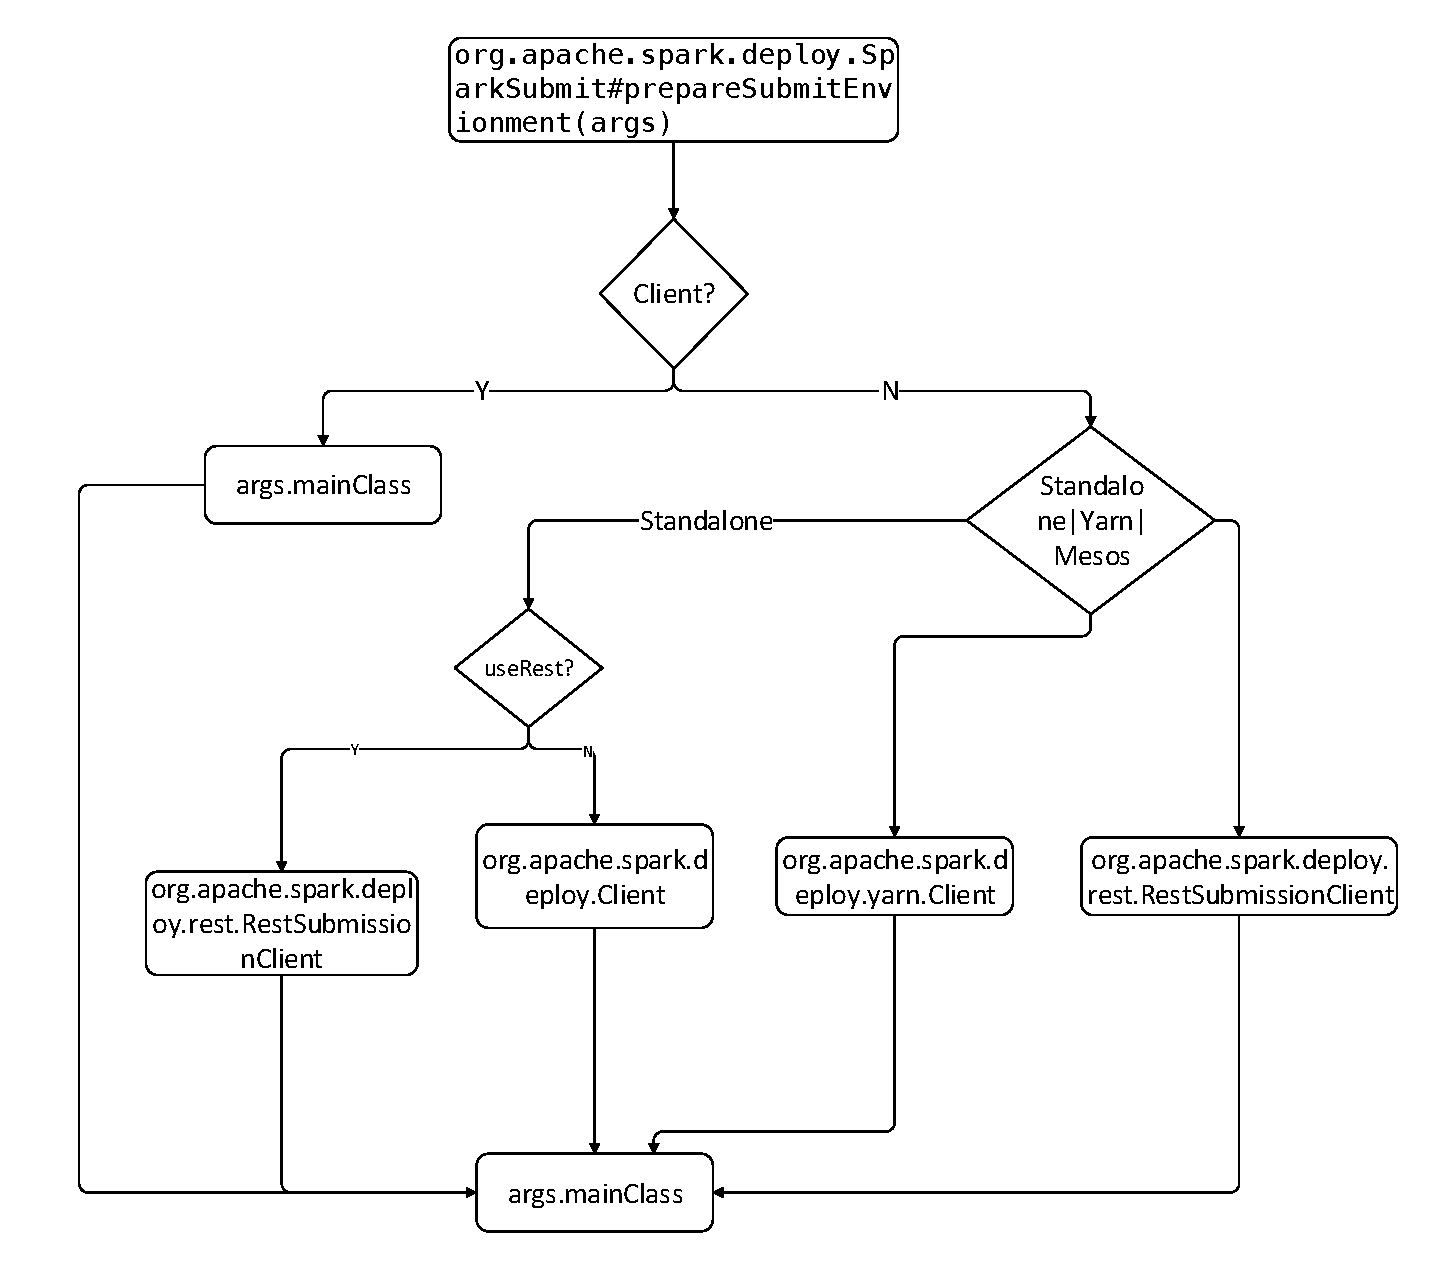
\includegraphics[scale=0.55]{figures/prepareSubmit.pdf}
     		\caption{prepareSubmit运行流程}
     		\label{prepareSubmit}
        	\end{figure}
为了验证自己分析的正确性,通过中间输出调试的方式,分别输出了在yarn-cluster和yarn-client模式下该方法返回的四元组值,命令为最前面的命令,其结果如表\ref{tab:deploymode}所示
           \begin{table}[t]
           	\caption{Yarn-Cluster和Yarn-Client模式下的参数对比}
      		\label{tab:deploymode}
      		\begin{tabularx}{\linewidth}{p{2.5cm}XX}
      			\toprule[1.5pt]
      			{\heiti 参数名} & {\heiti Yarn-Cluster} &{\heiti Yarn-Client}\\
      			\midrule[1pt]
      		childArgs&&ArrayBuffer(/user/root/inputfile.txt, 2)\\
      		childClasspath&ArrayBuffer()&ArrayBuffer(file:/root/HelloWorld-1.0-SNAPSHOT-jar-with-dependencies.jar)\\
      		sysProps&很多,基本都是系统属性&spark.master->yarn-client\\
      		childMainClass&org.apache.spark.deploy.yarn.Client&com.wtx.HelloWorld\\
      		\bottomrule[1.5pt]
      		\end{tabularx}
          \end{table}
       由结果可知,我们的分析是正确的。
       这里我们使用的master为yarn,deploy-mode为cluster,所以childMainClass为org.apache.spark.deploy.yarn.Client。
       \item 对于runMain
       \begin{enumerate}
       	\item 先检查查是否可见,是的话打印出各个参数的配置信息;
       	\item 跟据spark.driver.userClassPathFirst这个属性确定类加载器,这个属性可以降低Spark依赖和用户依赖的冲突。它现在还是一个实验性的特征;
       	\item 将jar包加入到类加载器的classpath;
       	\item 通过反射射的方式找到mainClass,然后在获得其main方法,并通过invoke加载main方法,这里就是org.apache.spark.deploy.yarn.Client的main方法。
       \end{enumerate}
     \end{enumerate}
\end{enumerate}
    到这里spark-submit就执行完了,接下来将分析org.apache.spark.deploy.yarn.Client的main方法执行过程。
\section{Yarn代理的启动}
由\ref{SparkSubmitMain}节我们知道,其最后就是反射加载org.apache.spark.deploy.yarn.Client的main方法,其执行过程如图\ref{fig:YarnClientMain}所示
	\begin{figure}[H] 
	\centering
	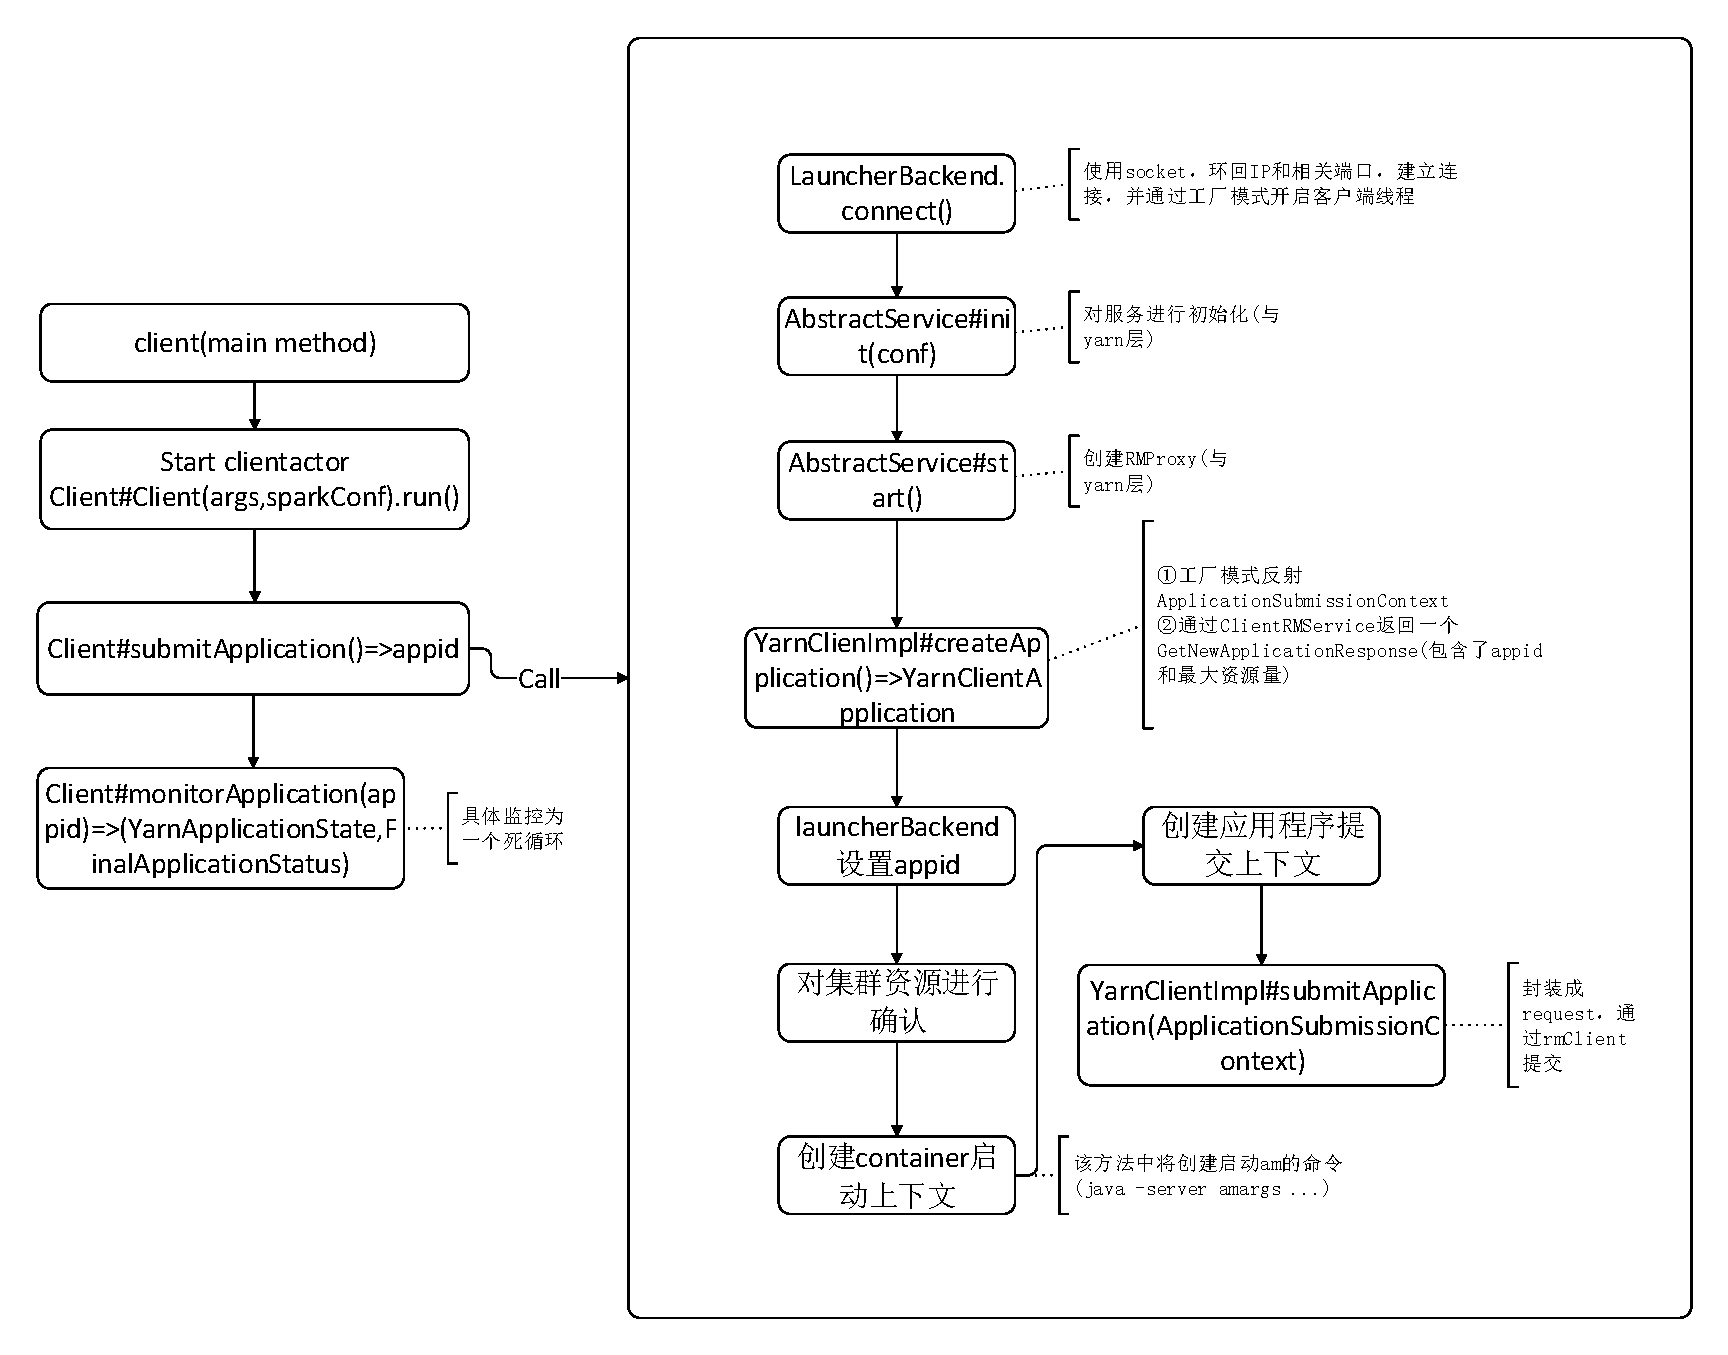
\includegraphics[width=\textwidth]{figures/YarnClientMain.pdf}
	\caption{YarnClientMain流程}
	\label{fig:YarnClientMain}
\end{figure}
main函数代码如程序\ref{fig:yarnclientmainscala}所示
\begin{lstlisting}[%
language=Scala,
caption={YarnClient中main函数},
label={fig:yarnclientmainscala}]
/**
* --name, com.wtx.HelloWorld,
* --jar, file:/root/HelloWorld-1.0-SNAPSHOT-jar-with-dependencies.jar,
* --class, com.wtx.HelloWorld,
* --arg, /user/root/inputfile.txt,
* --arg, 2
* */
def main(argStrings: Array[String]) {
	if (!sys.props.contains("SPARK_SUBMIT")) {
	logWarning("WARNING: This client is deprecated and will be removed in a " +
		"future version of Spark. Use ./bin/spark-submit with \"--master yarn\"")
	}
	System.setProperty("SPARK_YARN_MODE", "true")
	val sparkConf = new SparkConf
	val args = new ClientArguments(argStrings, sparkConf)
	if (!Utils.isDynamicAllocationEnabled(sparkConf)) {
		sparkConf.setIfMissing("spark.executor.instances", args.numExecutors.toString)
	}
	new Client(args, sparkConf).run()
}
\end{lstlisting}
这里面第一个执行的是ClientArguments方法,该方法中
\begin{itemize}
	\item[---] 对传入的参数进行解析,通过—标识符识别,像jar、class、arg之类的
	\item[---] 获取spark环境中的默认配置参数,就是获取spark.yarn.dist.files和spark.yarn.dist.archives这两个
	\item[---] 对已经解析出来的参数进行校验
\end{itemize}

之后就是Client中的主要方法,new Client(args, sparkConf).run()。

创建Client对象时,对一些变量如yarnClient、amMemoryOverhead、executorMemoryOverhead、isClusterMode等,其中yarnClient初始化为YarnClientImpl对象。
接着就是运行run方法。其代码如程序\ref{yarnclientrunscala}所示
\begin{lstlisting}[%
language=Scala,
caption={YarnClient中run函数},
label={yarnclientrunscala}]
def run(): Unit = {
	this.appId = submitApplication()
	if (!launcherBackend.isConnected() && fireAndForget) {
    	val report = getApplicationReport(appId)
    	val state = report.getYarnApplicationState
    	logInfo(s"Application report for $appId (state: $state)")
    	logInfo(formatReportDetails(report))
    	if (state == YarnApplicationState.FAILED || state == YarnApplicationState.KILLED) {
			throw new SparkException(s"Application $appId finished with status: $state")
		}
	} else {
    	val (yarnApplicationState, finalApplicationStatus) = monitorApplication(appId)
    	if (yarnApplicationState == YarnApplicationState.FAILED ||
      		finalApplicationStatus == FinalApplicationStatus.FAILED) {
     		 throw new SparkException(s"Application $appId finished with failed status")
    	}
    	if (yarnApplicationState == YarnApplicationState.KILLED ||
			finalApplicationStatus == FinalApplicationStatus.KILLED) {
      		throw new SparkException(s"Application $appId is killed")
    	}
    	if (finalApplicationStatus == FinalApplicationStatus.UNDEFINED) {
      		throw new SparkException(s"The final status of application $appId is undefined")
    	}
	}
}
\end{lstlisting}

run里第一个调用的方法就是Client\#submitApplication()方法,此方法最终返回的是与yarn通信之后的applicationId。
Client\#submitApplication()方法主要作用如下
\begin{itemize}
	\item launcher server进行连接
	\item   对sparkconf初始化,并创建对ResourceManager的代理客户端rmClient,以及开启historyClient和timelineClient(具体怎么建立代理会在下一部分详述,这里我们只需要理解成客户端操作服务端的方法就像操作本地的方法一样)
	\item 调用YarnClientImpl\#createApplication()与yarn上创建一个YarnClientApplication对象,其类图如图\ref{YarnClientApplication}所示,这里面包含了重要的appid等信息
		\begin{figure}[H] 
		\centering
		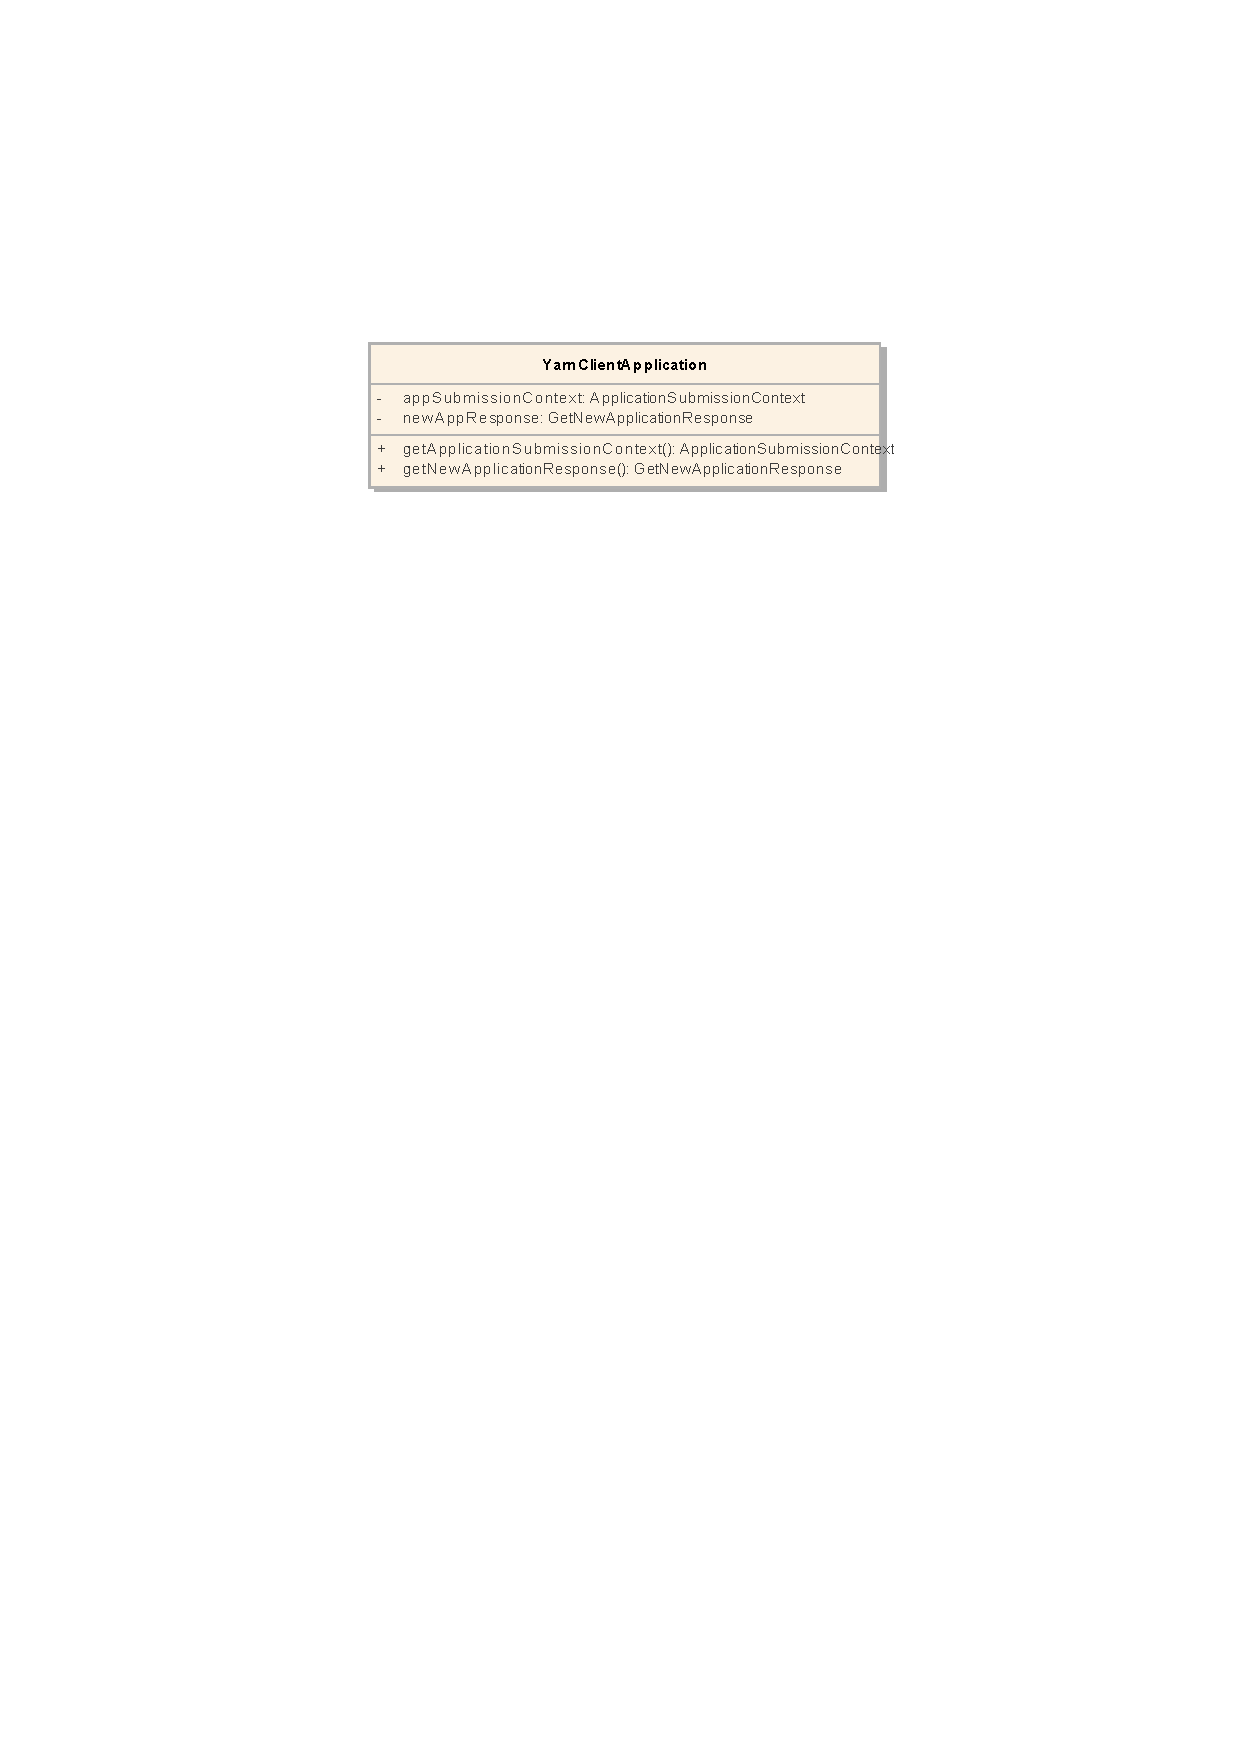
\includegraphics{figures/YarnClientApplication.pdf}
		\caption{YarnClientApplication类图}
		\label{YarnClientApplication}
	\end{figure}
	\item 核对集群上是否满足ApplicationMaster的资源要求
	\item 创建ApplicationMaster的Container启动上下文信息,这里面将上传三种文件到hdfs对应的目录,分别为spark-hdp-assemably、我们编写的spark应用jar包以及spark配置信息,之后将为amContainer封装一个启动AM\footnote{AM为ApplicationMaster的简写,以后本文中的AM不做特殊说明,均指代ApplicationMaster}的命令,类似于java -server 这样的
	\item 创建提交AM的上下文信息,包括spark应用名称、AM内存以及扩展值、AM虚拟核数等信息
	\item 将AM上下文信息提交到ResourceManager
\end{itemize}

run里面第二个调用就是monitorApplication(ApplicationId)。此函数通过Client\#submitApplication()方法返回的appid实现对提交spark应用的监控,在实现上通过一个死循环,让客户端线程每隔spark.yarn.report.interval中定义的时间进行应用执行状态的获取,然后显示在客户端控制台上。应用执行状态(ACCEPTED之后)即为以下四种的一种,FINISHED, FAILED,KILLED或者RUNNING。程序最终执行状态定义为以下四种UNDEFINED, SUCCEEDED, FAILED或KILLED。
\section{ApplicationMaster的启动}
前面通过yarn的代理客户端提交文件和提交程序信息之后,由yarn来进行分配container\footnote{container为资源的抽象,包含CPU、内存、网络资源和硬盘,Yarn中负责分配CPU和内存}给am,并将am的上下文信息发送给包含amContainer的nodeManager,由其来启动am。am的main函数如程序\ref{ammain}所示
\begin{lstlisting}[%
language=Scala,
caption={ApplicationMaster中main函数},
label={ammain}]
def main(args: Array[String]): Unit = {
	SignalLogger.register(log)
	val amArgs = new ApplicationMasterArguments(args)
	SparkHadoopUtil.get.runAsSparkUser { () =>
    	master = new ApplicationMaster(amArgs, new YarnRMClient(amArgs))
    	System.exit(master.run())
	}
}
\end{lstlisting}

在spark源码中am由单例对象和伴生类组成,main函数的处理过程如下
\begin{itemize}
	\item 对传入am的参数进行解析封装成ApplicationMasterArguments,其类图如图\ref{ApplicationMasterArguments}所示
\begin{figure}[H] 
	\centering
	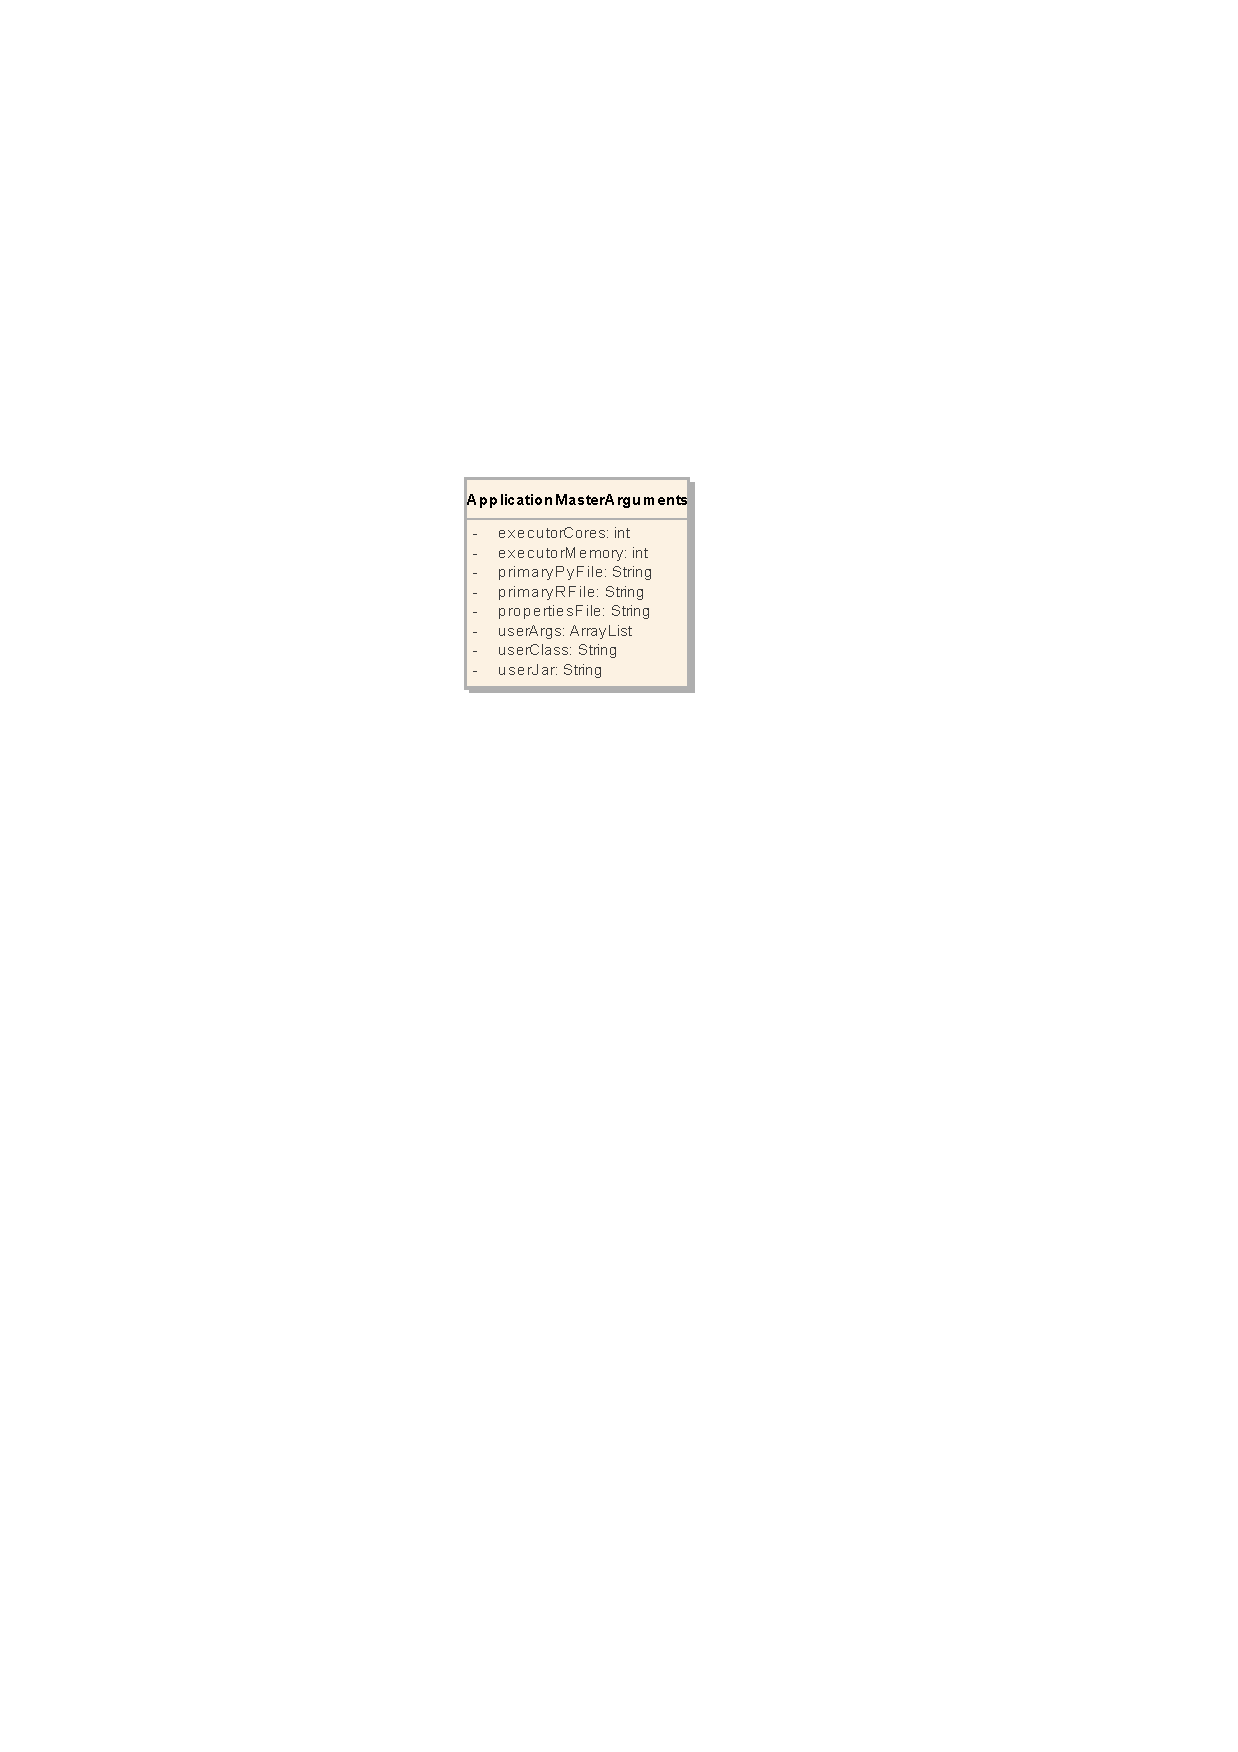
\includegraphics{figures/ApplicationMasterArguments.pdf}
	\caption{ApplicationMasterArguments类图}
	\label{ApplicationMasterArguments}
\end{figure}
	\item 实例化ApplicationMaster,这里实例的是ApplicationMaster的伴生类,因为单例对象是不能实例化的,且我们要注意实例化ApplicationMasterArguments
	ApplicationMaster传入的第二个参数为YarnRMClient,这个负责在yarn上注册或者取消Application
	\item 执行ApplicationMaster的run方法,此方法首先获取yarn的配置信息,然后对Application进行注册,接着判断是否为cluster模式,是的话就是启动driver,否则启动executor
\end{itemize}
\section{Driver的启动}
Yarn-Cluster模式下Driver的启动过程如图\ref{fig:startDriver}所示
\begin{figure}[H]
	\centering
		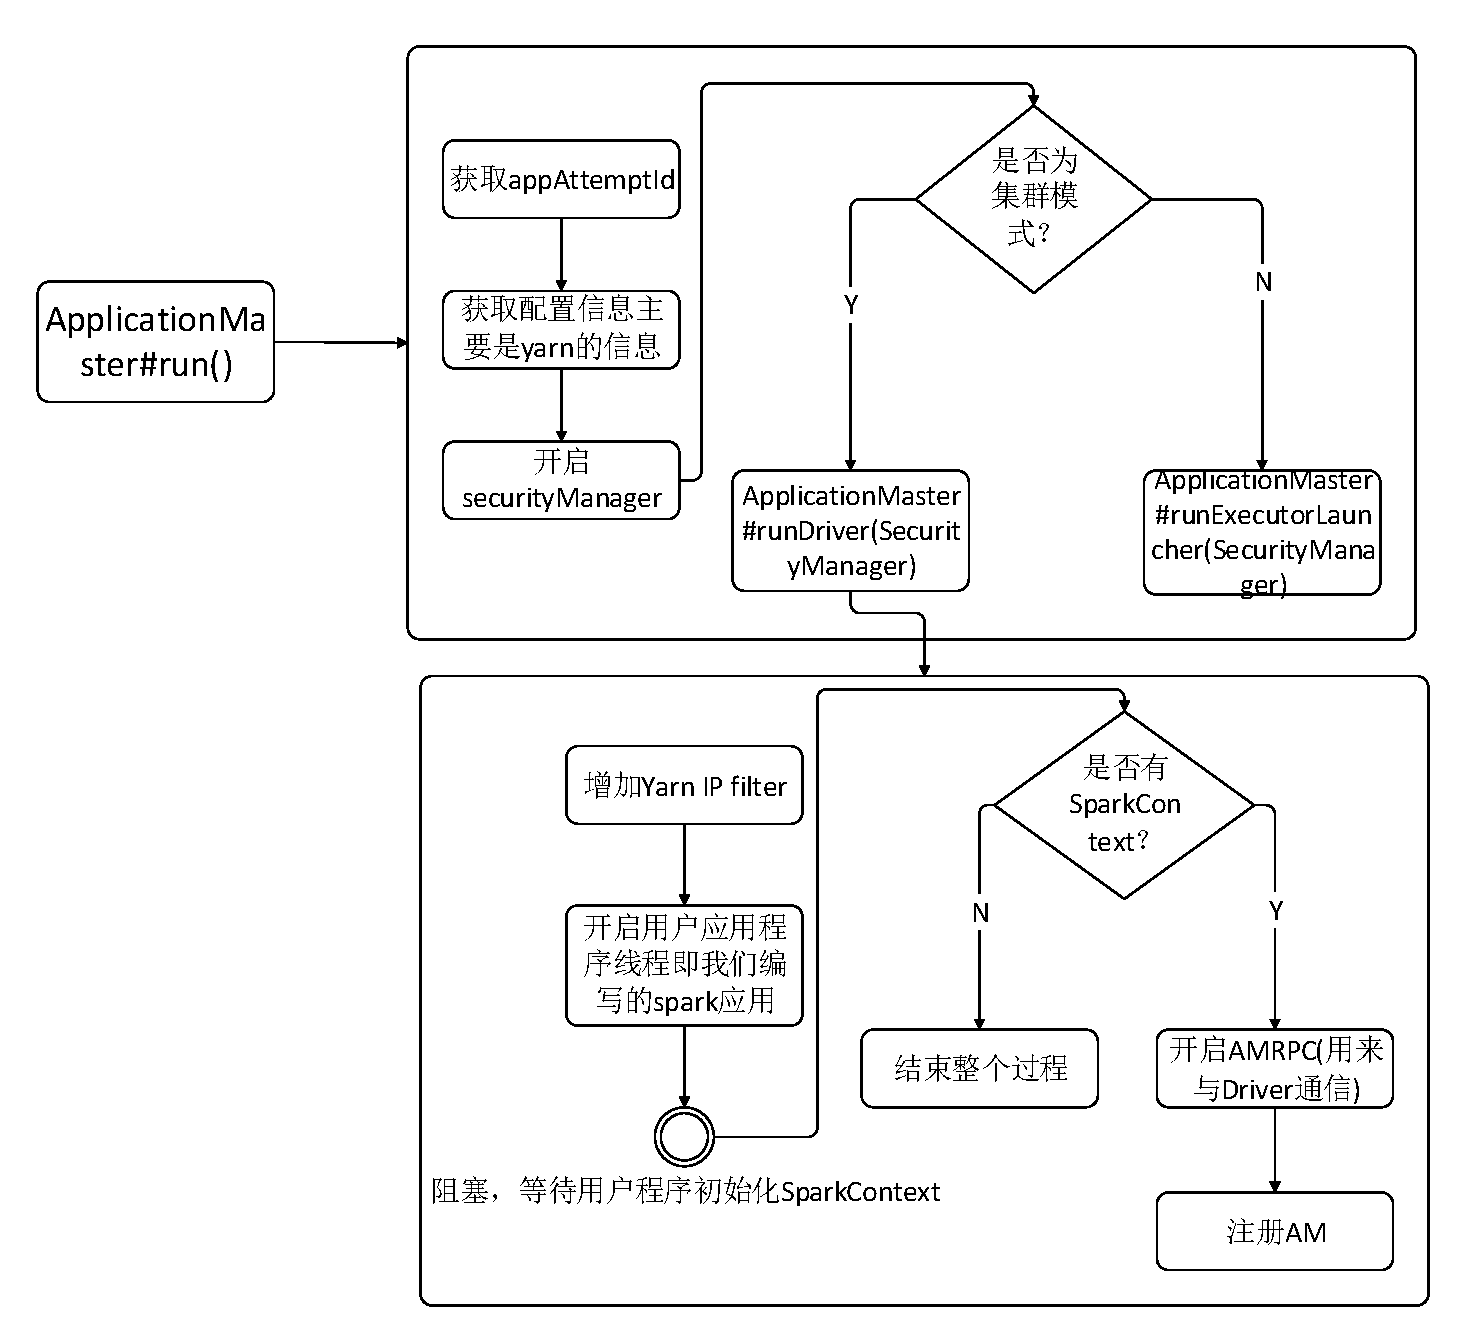
\includegraphics[width=\textwidth]{figures/startDriver.pdf}
	\caption{Driver启动过程}
	\label{fig:startDriver}
\end{figure}

启动Dirver的程序如程序\ref{lst:rundriver}所示
\begin{lstlisting}[%
language=Scala,
caption={启动Driver},
label={lst:rundriver}]
private def runDriver(securityMgr: SecurityManager): Unit = {
    addAmIpFilter()
    userClassThread = startUserApplication()
    val sc = waitForSparkContextInitialized()
    if (sc == null) {
        finish(FinalApplicationStatus.FAILED,
        ApplicationMaster.EXIT_SC_NOT_INITED,
        "Timed out waiting for SparkContext.")
    } else {
        rpcEnv = sc.env.rpcEnv
        val driverRef = runAMEndpoint(
        sc.getConf.get("spark.driver.host"),
		sc.getConf.get("spark.driver.port"),
		isClusterMode = true)
		registerAM(rpcEnv, driverRef, sc.ui.map(_.appUIAddress).getOrElse(""), securityMgr)
		userClassThread.join()
	}
}
\end{lstlisting}

从源码中可以看到启动Driver的第一步为启动用户程序\footnote{这里的用户程序即为我们所编写的WorldCount程序},这里面对启动用户程序做了配置,具体如下
\begin{itemize}
	\item 获得用户程序所需要的ClassPath
	\item 获取类加载器信息
	\item 获得用户jar包路径
	\item 获得用户程序主类参数列表
	\item 开启一个新的线程,通过反射机制,以用户程序主类主函数为入口,加载用户程序
\end{itemize}

在用户程序主类的运行过程中,此时主线程\footnote{指AM进程中运行Driver的线程}会阻塞,等待用户程序SparkContext初始化完成。
\chapter{SparkContext的初始化}
\label{scinitial}
Driver线程启动子线程来加载用户程序主类,主类中第一步是对SparkContext的初始化,SparkContext可以算得上是所有用户程序的启动引擎。而SparkContext初始化的配置参数由SparkConf负责。
\section{执行环境SparkConf}
SparkConf的构造很简单,主要包含的是提交用户程序的参数信息,包括setMaster、setAppName等。Spark的配置属性都是以“Spark.”开头的字符串。下面介绍SparkConf中重要的方法
\begin{enumerate}[\bfseries 1]
	\item registerKryoClasses
	
	注册时使用Kryo序列化的类,指定该类的序列化器为Kryo,关于Kryo的使用是spark性能优化的一个重要的组成部分。其中一个简单的应用是图计算。
	\item registerAvroSchemas
	
	序列化前先对Schema进行注册,影响的是压缩效率。
\end{enumerate}
\section{SparkContext综合概述}
配置完的SparkConf传入SparkContext,将SparkContext比作汽车发动机的引擎,SparkConf就是我们的控制面板,SparkContext中的SparkEnv创建一些Spark应用运行必备的组件,像Rpc、序列化器、块管理器、缓存管理器、测量系统、中间数据追踪器及文件服务器等,可以理解为汽车的空调、电路、油门线等环境条件。SparkContext和SparkEnv关系可以表示为
\tcbset{colback=red!5!white,colframe=red!75!black}
\tcbsetforeverylayer{colframe=red!75!black}
\begin{tcolorbox}[title=SparkContect]
	\begin{tabularx}{\linewidth}{XXXX}
		callSite&listenerBus&\_metadataCleaner&\_statusTracker\\
		SparkUI&\_dagScheduler&\_schedulerBackend&\_taskScheduler\\
	\end{tabularx}
	\begin{tcolorbox}[title=SparkEnv]
		\begin{tabularx}{\linewidth}{XXX}
			RpcEnv&serializer&closureSerializer\\
			mapOutputTracker&shuffle类型&blockManager(master)\\
			broadcastManager&cacheManager&metricsSystem\\
		\end{tabularx}
	\end{tcolorbox}
\end{tcolorbox}
\subsection{调用栈}
CallSite中存储了线程栈中最靠近栈顶的用户类以及最靠近栈底的Scala或者Spark核心类,这个变量其实主要是给开发者看的,对于具体程序的运行没有必然的影响。当然它的信息也会反应在SparkUI的界面上的。
\subsection{监听主线ListenerBus}
Spark消息系统的具体实现为后台会自动开启一个线程来监听事件,现在基本上所有的分布式系统都是通过消息驱动的方式来进行并发执行的。具体的线程执行如程序\ref{inputPrg:listenerThread}所示,从源码中可以看出,它其实是一个守护进程,是通过一个死循环,对事件队列里所有的事件进行遍历,再将不同的事件发送给不同的监听器Listener。
\begin{codeInput}{Scala}{listenerBus程序代码片段}{listenerThread}
private val listenerThread = new Thread(name) {
  setDaemon(true)
  override def run(): Unit = Utils.tryOrStopSparkContext(sparkContext) {
    AsynchronousListenerBus.withinListenerThread.withValue(true) {
      while (true) {
        eventLock.acquire()
          self.synchronized {
            processingEvent = true
          }
        try {
          val event = eventQueue.poll
          if (event == null) {
            if (!stopped.get) {
              ......
            }
            return
          }
          postToAll(event)
        } finally {
          self.synchronized {
            processingEvent = false
          }
        }
      }
    }
  }
}
\end{codeInput}
\subsection{元数据清理器}
SparkContext中\_metadataCleaner为元数据清理器,SparkContext为了保持对所有持久化的RDD的跟踪,使用类型是TimeStampped-WeakValueHashMap的persistentRdds缓存。元数据清理器的功能就是清除过期的持久化的RDD。
\subsection{可视化监控服务SparkUI}
Spark UI提供监控功能,以具有样式和布局的网页形式来提供丰富的监控数据,通过浏览器就能进行访问。SparkUI的创建代码如程序\ref{inputPrg:sparkui}所示
\begin{codeInput}{Scala}{SparkUI声明}{sparkui}
    _ui =
    if (conf.getBoolean("spark.ui.enabled", true)) {
      Some(SparkUI.createLiveUI(this, _conf, listenerBus, _jobProgressListener,
      _env.securityManager, appName, startTime = startTime))
    } else {
      // For tests, do not enable the UI
      None
    }
    _ui.foreach(_.bind())
\end{codeInput}
这其中的createLiveUI,实际是调用了SparkUI\#create方法,create方法如程序\ref{inputPrg:sparkcreate}所示
\begin{codeInput}{Scala}{SparkUI创建方法}{sparkcreate}
private def create(
  sc: Option[SparkContext],
  conf: SparkConf,
  listenerBus: SparkListenerBus,
  securityManager: SecurityManager,
  appName: String,
  basePath: String = "",
  jobProgressListener: Option[JobProgressListener] = None,
  startTime: Long): SparkUI = {
    val _jobProgressListener: JobProgressListener = jobProgressListener.getOrElse {
    val listener = new JobProgressListener(conf)
    listenerBus.addListener(listener) listener
  }
  val environmentListener = new EnvironmentListener
  val storageStatusListener = new StorageStatusListener
  val executorsListener = new ExecutorsListener(storageStatusListener)
  val storageListener = new StorageListener(storageStatusListener)
  val operationGraphListener = new RDDOperationGraphListener(conf)	
  listenerBus.addListener(environmentListener)
  listenerBus.addListener(storageStatusListener)
  listenerBus.addListener(executorsListener)
  listenerBus.addListener(storageListener)
  listenerBus.addListener(operationGraphListener)		
  new SparkUI(sc, conf, securityManager, environmentListener, storageStatusListener,
  executorsListener, _jobProgressListener, storageListener, operationGraphListener,
  appName, basePath, startTime)
}
\end{codeInput}

可以看出这里除了JobProgressListener是外部传入的之外,又增加了SparkListener。最后创建SparkUI,SparkUI服务默认是可以被杀掉的,可以修改属性spark.ui.killEnabled为false可以保证不被杀死。类SparkUI构造方法通过调用initialize方法会组织前端各个Tab和Page的展示及布局。
SparkUI的页面布局和展示使用的是JobsTab。它可以展示所有的Job进度、状态信息,这里我们以它为例,JobsTab会复用SparkUI的killEnabled、SparkContext、jobProgressListener,包括AllJobsPage和JobPage两个页面,JobsTab类实现代码程序\ref{inputPrg:jobstab}所示
\begin{codeInput}{Scala}{SparkUI JobsTab}{jobstab}
private[ui] class JobsTab(parent: SparkUI) extends SparkUITab(parent, "jobs") {
  val sc = parent.sc
  val killEnabled = parent.killEnabled
  val jobProgresslistener = parent.jobProgressListener
  val executorListener = parent.executorsListener
  val operationGraphListener = parent.operationGraphListener		
  def isFairScheduler: Boolean =
    jobProgresslistener.schedulingMode.exists(_ == SchedulingMode.FAIR)	
      attachPage(new AllJobsPage(this))
      attachPage(new JobPage(this))
  }
\end{codeInput}

第一个就是AllJobsPage,它由render方法进行渲染,利用jobProgressListener中统计监控数据生成激活、完成、失败等状态Job摘要信息,并调用jobsTable方法生成html各元素,最终使用UIUtils的headerSparkPage封装好css、js、header及页面布局等。 渲染方法部分代码如程序\ref{inputPrg:render}所示
\begin{codeInput}{Scala}{渲染方法实现}{render}
def render(request: HttpServletRequest): Seq[Node] = {
  progressListener.synchronized {
    ......
    val stageHeader = s"Details for Stage $stageId (Attempt $stageAttemptId)"
    if (stageDataOption.isEmpty) {
      val content =
      <div id="no-info">
      <p>No information to display for Stage {stageId} (Attempt {stageAttemptId})</p>
      </div>
      return UIUtils.headerSparkPage(stageHeader, content, parent)	
    }
    if (stageDataOption.get.taskData.isEmpty) {
      val content =
      <div>
      <h4>Summary Metrics</h4> No tasks have started yet
      <h4>Tasks</h4> No tasks have started yet
      </div>
      return UIUtils.headerSparkPage(stageHeader, content, parent)
  }	
  val stageData = stageDataOption.get
  val tasks = stageData.taskData.values.toSeq.sortBy(_.taskInfo.launchTime)
  val numCompleted = tasks.count(_.taskInfo.finished)
  val allAccumulables = progressListener.stageIdToData((stageId, stageAttemptId)).accumulables
  val externalAccumulables = allAccumulables.values.filter { acc => !acc.internal }
  val hasAccumulators = externalAccumulables.size > 0			
  val summary =
  <div>
  <ul class="unstyled">
  <li>
  <strong>Total Time Across All Tasks: </strong>
  {UIUtils.formatDuration(stageData.executorRunTime)}
  </li>
  <li>
  <strong>Locality Level Summary: </strong>
  {getLocalitySummaryString(stageData)}
  </li>
  ......
\end{codeInput}

SparkUI创建好后,需要调用父类的WebUI的bind方法,绑定服务和端口,绑定实现代码如程序\ref{inputPrg:bindsparkui}所示
\begin{codeInput}{Scala}{SparkUI绑定实现}{bindsparkui}
  /** Bind to the HTTP server behind this web interface. */
  def bind() {
    assert(!serverInfo.isDefined, "Attempted to bind %s more than once!".format(className))
    try {
      var host = Option(conf.getenv("SPARK_LOCAL_IP")).getOrElse("0.0.0.0")
      serverInfo = Some(startJettyServer(host, port, handlers, conf, name))
      logInfo("Bound %s to %s, and started at http://%s:%d".format(className, host,
        publicHostName, boundPort))
      } catch {
        case e: Exception =>
          logError("Failed to bind %s".format(className), e)
          System.exit(1)
      }
  }
\end{codeInput}
\subsection{任务调度器}
任务调度器组件由\_schedulerBackend和\_taskScheduler组成,在Spark框架中占据重要的地位,它们决定着Spark程序的整体运行流程,对应不同的资源管理方法和部署模式会有不同的实现。本文以Yarn-Cluster模式进行叙述。

SparkContext调用createTaskScheduler方法,该方法返回值为一个二元组,其元素由Scheduler和SchedulerBackend组成,此方法执行时通过模式匹配的方式进行,Yarn-Cluster模式下的匹配代码如程序\ref{inputPrg:matchyarnclusrer}所示
\begin{codeInput}{Scala}{匹配Yarn-Cluster}{matchyarnclusrer}
case "yarn-standalone" | "yarn-cluster" =>
  if (master == "yarn-standalone") {
    logWarning(
    "\"yarn-standalone\" is deprecated as of Spark 1.0. Use \"yarn-cluster\" instead.")
  }
  val scheduler = try {
    val clazz = Utils.classForName("org.apache.spark.scheduler.cluster.
    YarnClusterScheduler")
    val cons = clazz.getConstructor(classOf[SparkContext])
    cons.newInstance(sc).asInstanceOf[TaskSchedulerImpl]
  } catch {
  case e: Exception => {
    throw new SparkException("YARN mode not available ?", e)
  }
}
val backend = try {
  val clazz =Utils.classForName("org.apache.spark.scheduler.cluster.
  YarnClusterSchedulerBackend")
  val cons = clazz.getConstructor(classOf[TaskSchedulerImpl], classOf[SparkContext])
  cons.newInstance(scheduler, sc).asInstanceOf[CoarseGrainedSchedulerBackend]
} catch {
  ......
  }
}
scheduler.initialize(backend)
(backend, scheduler)
\end{codeInput}
Yarn-Cluster模式下两个组件分别得到下列值
\begin{centertitlebox}{Yarn-Cluster模式}
\_schedulerBackend=YarnClusterSchedulerBackend(extends YarnSchedulerBackend)\\   \_taskScheduler=YarnClusterScheduler(extends YarnScheduler)
\end{centertitlebox}
\begin{enumerate}[\bfseries 1]
	\item YarnClusterScheduler调度器
	
	其类图如图\ref{fig:YarnScheduler}所示
	\begin{figure}[H] 
		\centering
		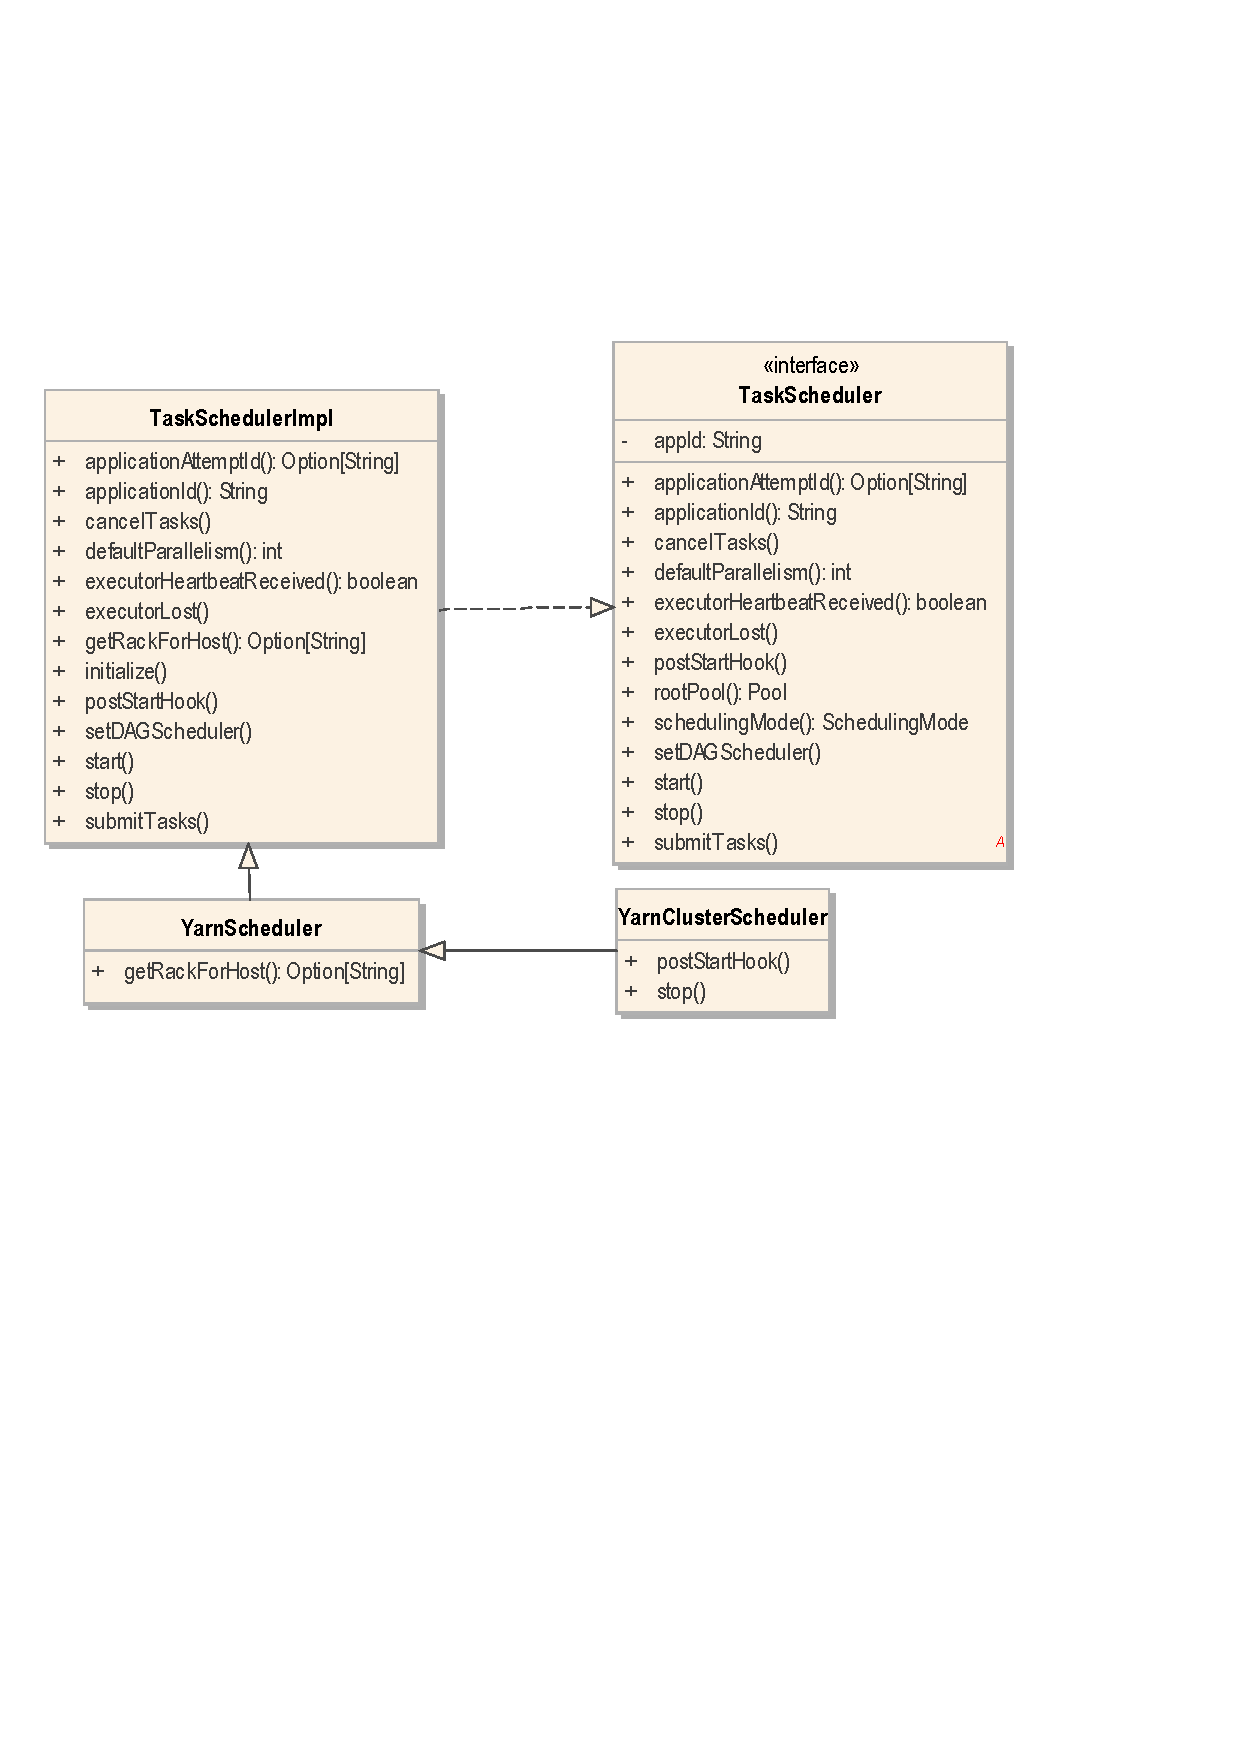
\includegraphics[width=\textwidth]{figures/YarnScheduler.pdf}
		\caption{YarnScheduler类图}
		\label{fig:YarnScheduler}
	\end{figure}

程序\ref{inputPrg:matchyarnclusrer}中倒数第二行代码,Scheduler调用initialize方法对backend进行绑定,我们可以从类图\ref{fig:YarnScheduler}看到实际上是调用了TaskSchedulerImpl\#initialize()方法,此方法代码很简短,指定JOb的调度模式,如程序\ref{inputPrg:taskschedulerimpl}所示
\begin{codeInput}{Scala}{调度器初始化实现}{taskschedulerimpl}
def initialize(backend: SchedulerBackend) {
  this.backend = backend
  rootPool = new Pool("", schedulingMode, 0, 0)
  schedulableBuilder = {
    schedulingMode match {
      case SchedulingMode.FIFO =>
      new FIFOSchedulableBuilder(rootPool)
      case SchedulingMode.FAIR =>
        new FairSchedulableBuilder(rootPool, conf)
      }
    }
    schedulableBuilder.buildPools()
}
\end{codeInput}


此方法最重要的作用就是将Scheduler和SchedulerBackend进行绑定,并制定Job的调度模式,当然默认情况下为FIFO。

接着执行\_taskScheduler.start(),由类图\ref{fig:YarnScheduler}可知实际上调用的是TaskSchedulerImpl\#start()方法,此方法代码如程序\ref{inputPrg:starttaskscheduler}所示,此方法首先调用YarnClusterSchedulerBackend\#start(),之后判断是否需要检查慢服务。
\begin{codeInput}{Scala}{开启任务调度器}{starttaskscheduler}
override def start() {
  //Yarn-cluster模式下为YarnClusterSchedulerBackend
  backend.start()	
    if (!isLocal && conf.getBoolean("spark.speculation", false)) {
      speculationScheduler.scheduleAtFixedRate(new Runnable {
        override def run(): Unit = Utils.tryOrStopSparkContext(sc) {
          checkSpeculatableTasks()
        }
      }, SPECULATION_INTERVAL_MS, SPECULATION_INTERVAL_MS, TimeUnit.MILLISECONDS)
    }
}
\end{codeInput}
	\item YarnClusterSchedulerBackend相关
	
	与其相关的类及接口如图\ref{fig:YarnSchedulerBackend}所示
	\begin{figure}[H] 
		\centering
		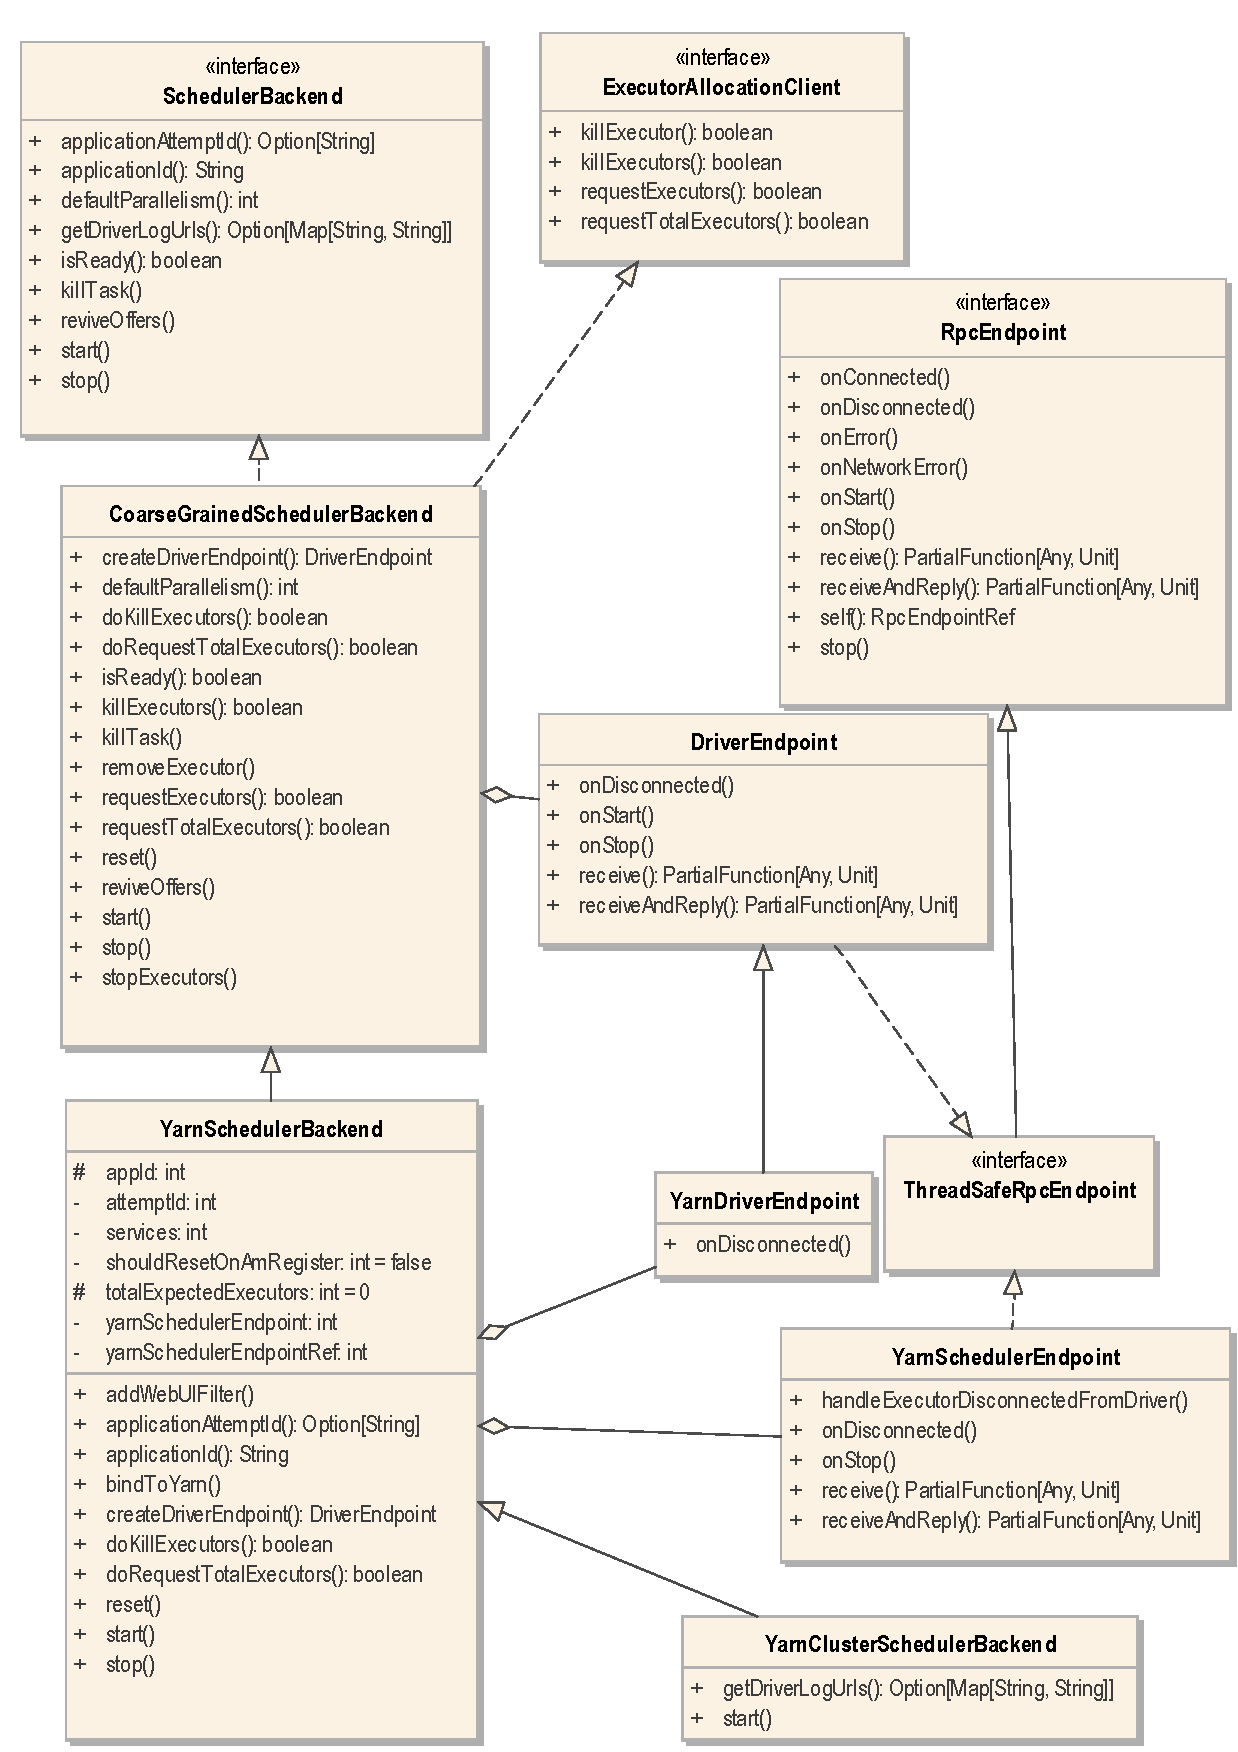
\includegraphics[width=\textwidth]{figures/YarnSchedulerBackend.pdf}
		\caption{YarnSchedulerBackend类图}
		\label{fig:YarnSchedulerBackend}
	\end{figure}
	接着从TaskSchedulerImpl\#start()方法,该方法中第一行即执行YarnClusterSchedulerBackend\#start(),作用为,将appid和attemptId绑定到Yarn上;调用父类的YarnSchedulerBackend\#start()方法。
	
	
	YarnSchedulerBackend\#start()方法:验证appid是否已经定义;Yarn-Cluster模式下,绑定SchedulerExtensionServiceBinding;调用父类CoarseGrainedSchedulerBackend\#start()方法;
	
	CoarseGrainedSchedulerBackend\#start()方法如程序\ref{inputPrg:CoarseGrainedScheduler}所示
	\begin{codeInput}{Scala}{开启CoarseGrainedScheduler}{CoarseGrainedScheduler}
  override def start() {
    val properties = new ArrayBuffer[(String, String)]
    for ((key, value) <- scheduler.sc.conf.getAll) {
      if (key.startsWith("spark.")) {
        properties += ((key, value))
      }
    }		
    // TODO (prashant) send conf instead of properties
    driverEndpoint = rpcEnv.setupEndpoint(ENDPOINT_NAME, createDriverEndpoint(properties))
}
\end{codeInput}

程序\ref{inputPrg:CoarseGrainedScheduler}中RPC在SparkContext\#createSparkEnv函数调用里,具体函数实现流程如图\ref{fig:RPCinitialize}所示。
\begin{figure}[H] 
	\centering
	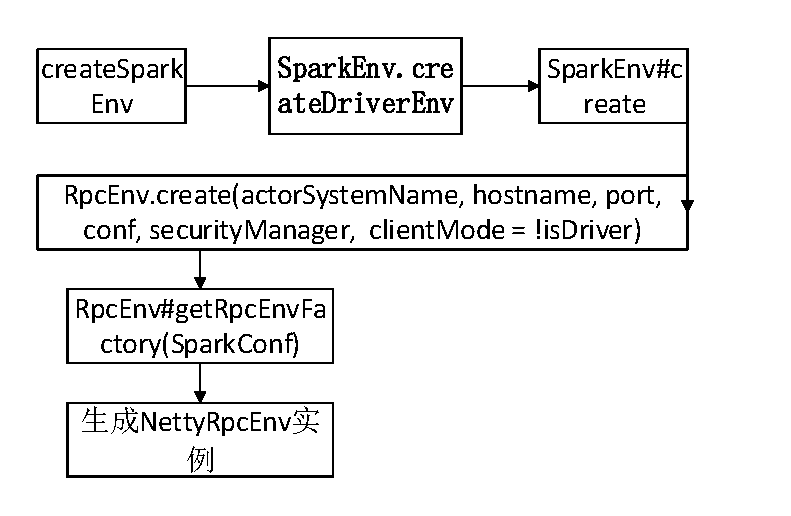
\includegraphics[scale=0.9]{figures/RPCinitialize.pdf}
	\caption{RPC建立过程}
	\label{fig:RPCinitialize}
\end{figure}

流程图\ref{fig:RPCinitialize}可以看出SparkRPC是通过工厂模式反射生成NettyRpcEnv实例。那么CoarseGrainedSchedulerBackend\#start()最后一行就执行的是NettyRpcEnv\#setupEndpoint(),接着执行Dispatcher\#registerRpcEndpoint(),最后就返回了NettyRpcEndpointRef。
\end{enumerate}
\subsection{DAG调度器}
DAGScheduler用于构建Job阶段,将用户应用的DAG划分为不同的Stage,其中Stage由可以并发控制的一组Task构成,这些Task逻辑上完全相同,只是运行在不同的数据分区上。具体的内部实现原理会在Job构建章节中进行讲述。DAGScheduler的数据结构主要维护jobId和stageId的关系、Stage、ActiveJob,以及缓存的RDD的partitions的位置信息。DAGScheduler的数据结构如程序\ref{inputPrg:dagscheduler}所示
\begin{codeInput}{Scala}{DAG调度器数据结构}{dagscheduler}
  private[scheduler] val nextJobId = new AtomicInteger(0)
  private[scheduler] def numTotalJobs: Int = nextJobId.get()
  private val nextStageId = new AtomicInteger(0)
  private[scheduler] val jobIdToStageIds = new HashMap[Int, HashSet[Int]]
  private[scheduler] val stageIdToStage = new HashMap[Int, Stage]
  private[scheduler] val shuffleToMapStage = new HashMap[Int, ShuffleMapStage]
  private[scheduler] val jobIdToActiveJob = new HashMap[Int, ActiveJob]
  // Stages we need to run whose parents aren't done
  private[scheduler] val waitingStages = new HashSet[Stage]
  // Stages we are running right now
  private[scheduler] val runningStages = new HashSet[Stage]
  // Stages that must be resubmitted due to fetch failures
  private[scheduler] val failedStages = new HashSet[Stage]
  private[scheduler] val activeJobs = new HashSet[ActiveJob]
\end{codeInput}


在初始化DAGScheduler的时候,会调用eventProcessLoop\#start(),这个用于创建子线程一直运行的事件监听线程。其调用过程如下图\ref{fig:eventListener}所示
\begin{figure}[H] 
	\centering
	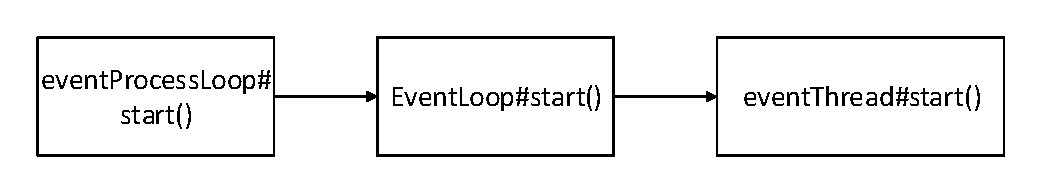
\includegraphics[width=\textwidth]{figures/eventListener.pdf}
	\caption{事件监听开启流程}
	\label{fig:eventListener}
\end{figure}

事件线程运行代码如程序\ref{inputPrg:eventListener}所示
\begin{codeInput}{Scala}{事件监听线程}{eventListener}
private val eventThread = new Thread(name) {
  setDaemon(true)	
  override def run(): Unit = {
    try {
      while (!stopped.get) {
        val event = eventQueue.take()
          try {
            onReceive(event)
          } catch {
            case NonFatal(e) => {
              ......
                }
              }
            }
          } catch {
            ......
        }
    }	
}
\end{codeInput}
从程序\ref{inputPrg:eventListener}中可以看出,事件监听器是个后台守护进程,其中运行的线程是一个由while循环组成的结构,其不断的从事件队列中取出事件,然后调用onReceive(event)方法对不同的事件进行模式匹配。这里的onReceive(event)是一个由子类实现的方法,如程序\ref{inputPrg:onReveive}所示
\begin{codeInput}{Scala}{DAGSchedulerEventProcessLoop.onReveive}{onReveive}
override def onReceive(event: DAGSchedulerEvent): Unit = {
  val timerContext = timer.time()
  try {
    doOnReceive(event)
  } finally {
    timerContext.stop()
  }
}
\end{codeInput}

程序中运行的是doOnReceive(DAGSchedulerEvent)方法,而这个方法中就包含了对不同事件的模式匹配以及对应着不同的处理方式。
\chapter{Spark RDD创建及转换}
\label{chap:rddcreate}
经过第\ref{scinitial}章SparkContext的初始化,Driver端会立即进行RDD的生成和转换。本章将按照WordCount实例对RDD生成和转换进行详解。
\section{Spark RDD综述}

RDD即为弹性数据集,它可以由存储在物理中的数据来生成,也可以通过其他RDD进行转换,RDD是Spark平台上的最基础的数据结构,分布式下可并行处理,并且对数据分区也可以根据业务不同进行改变,同时在系统内存资源足够的情况下,允许用户将计算中间结果缓存在内存中,后续的计算可以直接使用这个结果,这会极大的提高计算效能。

每个RDD内部,有下面5个主要的属性:

\begin{enumerate}[\bfseries 1]
	\item 数据分区列表
	
	为数据的基本组成单元,对于RDD来说,一个分区上将会对应一个计算任务,分区的个数会决定Job的并发度。在使用时可以由用户显示的指定分区数,没有指定的情况下,集群会采用默认的分区数,即集群工作节点上一个cpu core对应一个分区。分区的管理为BlockManager。
	
	RDD分区的个数如下公式所示
	\begin{equation}
		partitions = \max \{ blockSize, defaultMinPartition\}
	\end{equation}
    
    \begin{equation}
    defaultMinPartition=
    \begin{cases}
    textFile &\mbox{if 定义并行度}\\
    \min\{\max\{totalCores,2\},2\}
    \end{cases}
    \end{equation}
	\item 每个分区上的计算函数
	
	Spark中每个RDD都会实现一个computer函数,computer函数会对迭代器进行连接,但不会保存每次连接运算的中间结果。
	\item 对其他RDD的依赖列表
	
	RDD的每次转换都会生成一个新的RDD,新生成RDD(子RDD)会将旧RDD(父RDD)加入依赖,并将依赖加入列表中,这样就会形成一条线连接起各个RDD,这条线也称作生命线(lineage)。
	\item (可选)一个分区器
	
	针对key-value的RDD,分区器按照RDD的键值对进行处理,父RDD中的键值对在子RDD中分到哪个分区,分区器有两种,分变为HashPartitioner和RangePartitioner。分区器不但决定了RDD本身的分区数量,也决定了子RDD中输出的分区数量。
	\item (可选)计算每个分区优先位置列表
	
	对于数据源存储在HDFS中的,此列表存储的就是每个分区所在的块的位置。
\end{enumerate}
\section{Spark RDD创建}

创建RDD的方式有两种,第一种从存储在物理设备上的数据集创建,常见的有本地文件系统、HDFS和HBase,第二种通过已经存储在RDD进行转换。WordCount实例中数据存放在HDFS中,通过textFile读取HDFS文件内容并创建HadoopRDD。
\section{Spark RDD转换}

Spark RDD中的所有转换都是惰性的,在触发动作之前都只做单纯的连接。WordCount实例中,在RDD创建后通过flatmap生成一个新的数据集,并传入map生成新的数据集,接着传入reduceByKey,再接着传入filter生成新的数据集,最后返回给Driver的是saveAsText处理后的数据集,而不是整个数据集。
\section{DAG的生成}

Spark根据用户提交的计算逻辑中RDD的转换和动作来生成RDD之间的依赖关系,同时这个计算链条也就成了逻辑上的DAG。
\subsection{RDD中依赖}

RDD中每个Dependency子类内部都会存储一个RDD对象,对应一个父RDD,如果一次转换操作有多个父RDD,就会对应产生多个Dependency对象,使用List存储,所有的Dependency对象存储在子RDD内部,通过遍历RDD内部的Dependency对象,就能获取该RDD所有依赖的父RDD。RDD中主构造函数声明了Dependency的类型,如程序\ref{inputPrg:mainContruRDD}所示,可见RDD的deps为Seq类型,且其中的元素为Dependency。
\begin{codeInput}{Scala}{RDD主构造函数}{mainContruRDD}
abstract class RDD[T: ClassTag](
  @transient private var _sc: SparkContext,
  @transient private var deps: Seq[Dependency[_]]
  ) extends Serializable with Logging {
    ......
}
\end{codeInput}
子RDD和父RDD的依赖关系有两种,即宽依赖和窄依赖。两种依赖最简单的理解如图\ref{fig:deps}所示
\begin{enumerate}[\bfseries 1]
	\item 宽依赖是指子RDD中的一个分区依赖于父RDD的多个分区
	\item 窄依赖是指子RDD中的一个分区依赖于父RDD的一个分区
\end{enumerate}
\begin{figure}[H] 
	\centering
	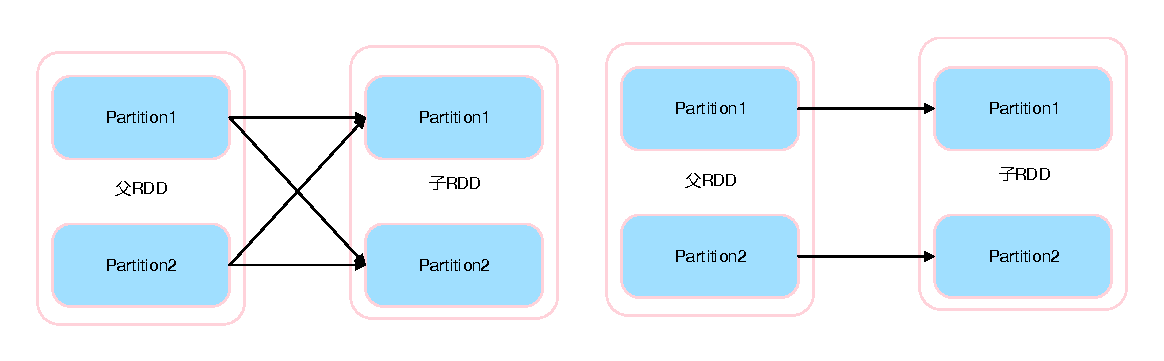
\includegraphics[width=\textwidth]{figures/wideandnarroewdeps.pdf}
	\caption{宽依赖(左)窄依赖(右)}
	\label{fig:deps}
\end{figure}

RDD不同的转换操作对应分区的映射规则不一样,但对于窄依赖而言计算任务作用于不同的数据分区,它们之间相互没有影响,所以这些计算任务也就可以并发的执行了。宽依赖中子RDD的单个分区要依赖父RDD的多个分区,因此这两个RDD不能通过一个计算任务来完成,这里需要进行shuffle。

RDD中依赖的层次图如图\ref{fig:depsclass}所示
\begin{figure}[H] 
	\centering
	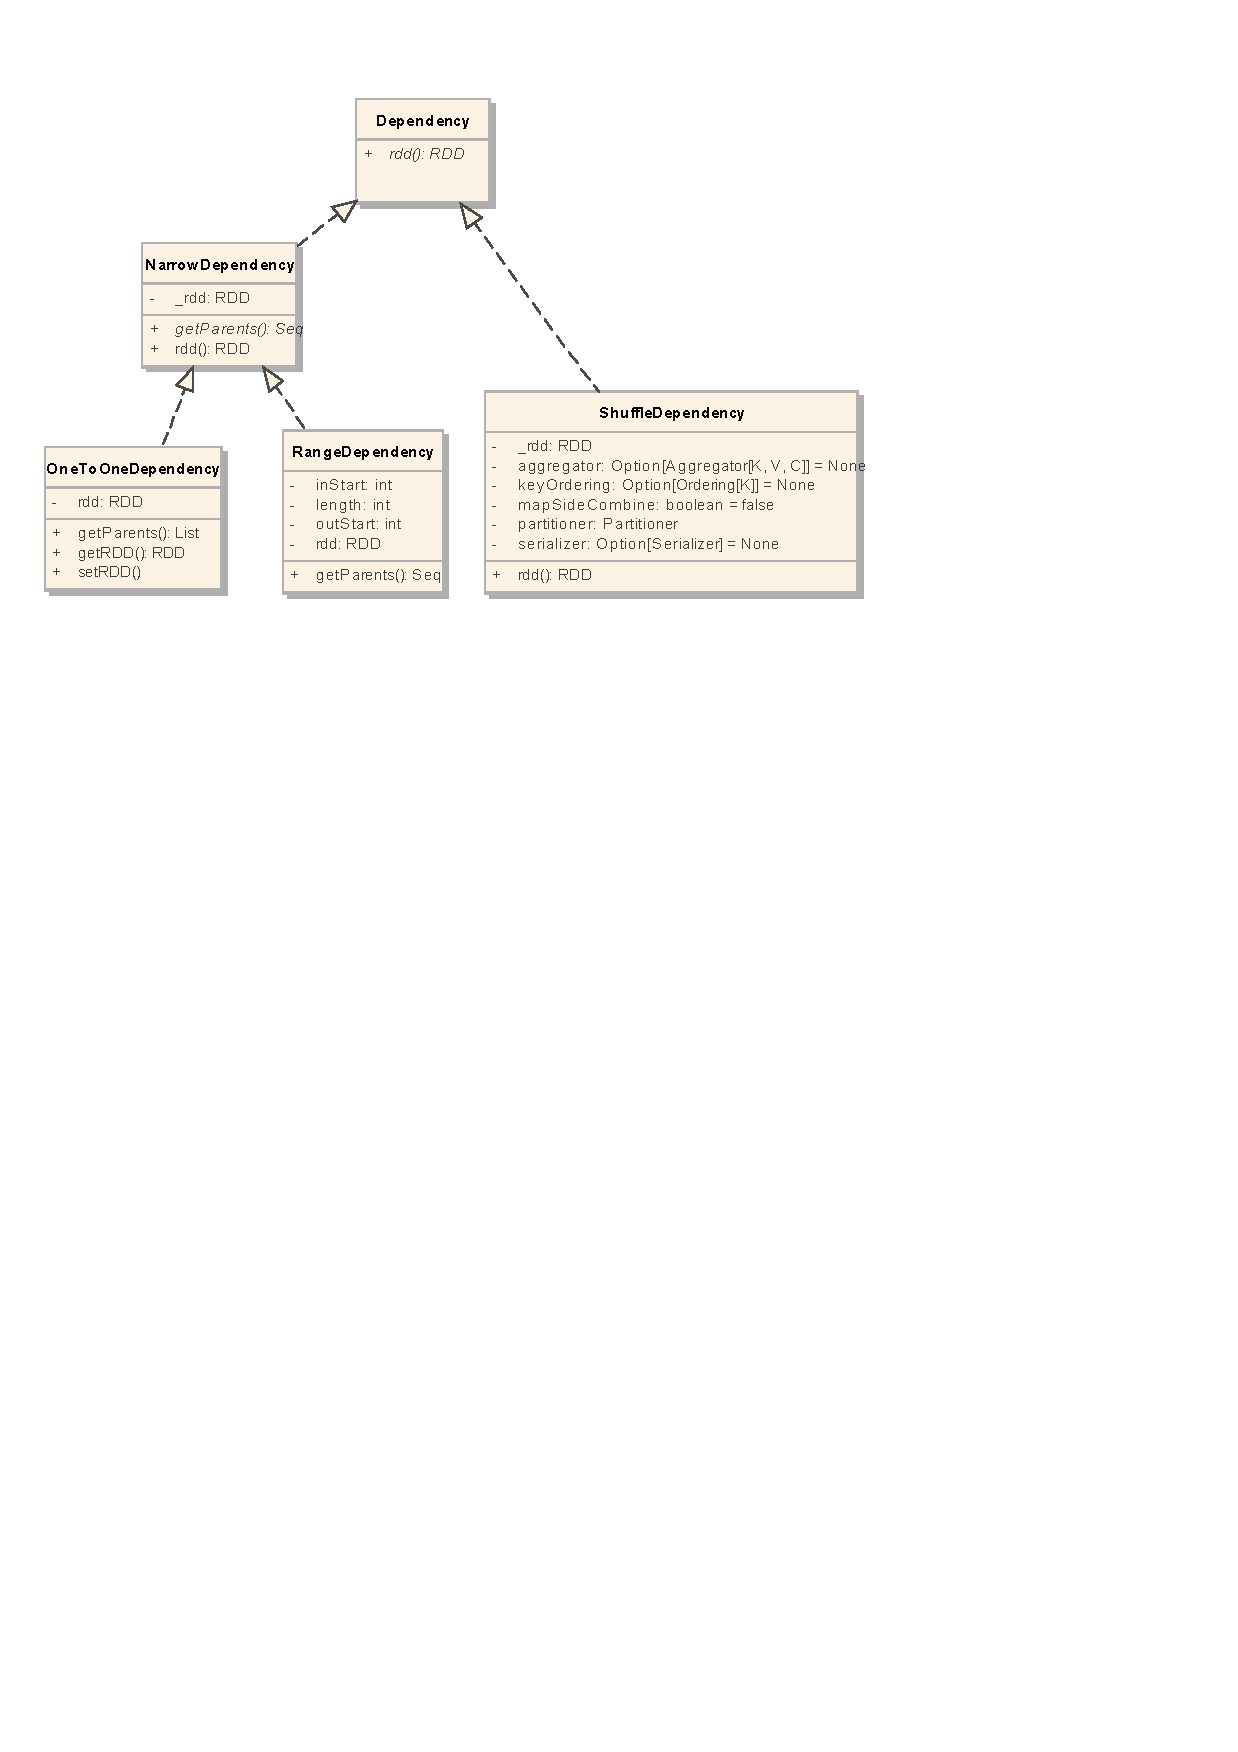
\includegraphics[width=\textwidth]{figures/dependencyclassl.pdf}
	\caption{Spark RDD依赖类层次图}
	\label{fig:depsclass}
\end{figure}
所有的依赖都要实现抽象类Dependency,其代码如程序\ref{inputPrg:abstractdeps}所示
\begin{codeInput}{Scala}{抽象类Dependency}{abstractdeps}
abstract class Dependency[T] extends Serializable {
  def rdd: RDD[T]
}
\end{codeInput}
这其中的rdd即为参数此RDD的父RDD,此为抽象方法,在子类中都必须有其实现。

窄依赖的实现如程序\ref{inputPrg:abstractnarrowdeps}所示
\begin{codeInput}{Scala}{NarrowDependency}{abstractnarrowdeps}
abstract class NarrowDependency[T](_rdd: RDD[T]) extends Dependency[T] {
  def getParents(partitionId: Int): Seq[Int]
  override def rdd: RDD[T] = _rdd
}
\end{codeInput}
这其中实现了对父RDD中rdd方法的实现,同时定义了一个抽象方法getParents,获取该依赖对应的父RDD的分区。

对于窄依赖的实现有两种,一种是OneToOneDependency,另一种是RangeDependency,这两种依赖都实现了getParents方法,只不过OneToOneDependency中父RDD和子RDD中的分区ID是相同的,RangeDependency仅仅被org.apache.spark.UnionRDD所使用,针对的是子RDD有多个父RDD的情形,但一对父子RDD中,分区任然是一对一,这种情形下依赖如图\ref{fig:rangedeps}所示
\begin{figure}[H] 
	\centering
	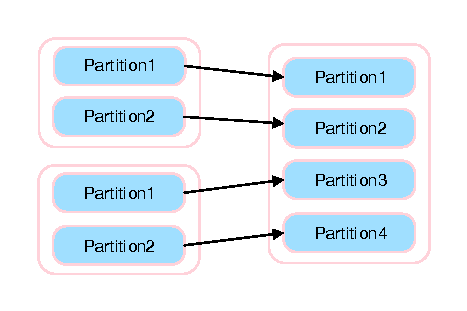
\includegraphics[scale=1.5]{figures/rangedeps.pdf}
	\caption{RangeDependency示例}
	\label{fig:rangedeps}
\end{figure}

宽依赖只有一种实现:ShuffleDependency,其代码如程序\ref{inputPrg:widedeps}所示
\begin{codeInput}{Scala}{ShuffleDependcy}{widedeps}
class ShuffleDependency[K: ClassTag, V: ClassTag, C: ClassTag](
  @transient private val _rdd: RDD[_ <: Product2[K, V]],
  val partitioner: Partitioner,
  val serializer: Option[Serializer] = None,
  val keyOrdering: Option[Ordering[K]] = None,
  val aggregator: Option[Aggregator[K, V, C]] = None,
  val mapSideCombine: Boolean = false)
    extends Dependency[Product2[K, V]] {	
      override def rdd: RDD[Product2[K, V]] = _rdd.asInstanceOf[RDD[Product2[K, V]]]
      private[spark] val keyClassName: String = reflect.classTag[K].runtimeClass.getName
      private[spark] val valueClassName: String = reflect.classTag[V].runtimeClass.getName
      private[spark] val combinerClassName: Option[String] =
      Option(reflect.classTag[C]).map(_.runtimeClass.getName)	
      val shuffleId: Int = _rdd.context.newShuffleId()
      val shuffleHandle: ShuffleHandle =
       _rdd.context.env.shuffleManager.registerShuffle(
        shuffleId,_rdd.partitions.size,this)
      _rdd.sparkContext.cleaner.foreach(
        _.registerShuffleForCleanup(this))
}
\end{codeInput}

这里处理了一些变量,为map端本地聚合做准备。shuffle的具体过程会在以后章节进行分析。
\subsection{DAG构建}

RDD通过一系列转换,会形成自己的依赖列表,列表中的每个依赖都会包含一个父RDD的对象,ShuffleRDD依赖中另外包含了分区器、序列化器、map端聚合等参数。这些信息提供了子RDD由那些父RDD转换而来以及它所依赖的父RDD的分区信息。逻辑上,各RDD通过一条线连接,且由子RDD指向父RDD,这样就形成了一条Lineage,也可看做这些RDD形成了DAG。

Spark根据由DAG来划分Stage,进而生成计算任务。在同一个分区上进行计算的任务可以放在一个线程中计算,而宽依赖中子RDD要从父RDD的各个分区中拉取数据,并且放到不同的分区中进行计算,所以得新开一个线程进行。由此可得出划分Stage的依据就是ShuffleDependency。划分阶段在RDD触发Action之后,具体分析会在调度章节进行说明。

\subsection{WordCount的RDD转换和DAG生成}

本实例中WordCount运行在三台主机构成的集群中,两台为NodeManager ,一台作为ResourceManager,输入数据保存在HDFS上,且存在DataNode中的某一台上,RDD转换的细节如图\ref{fig:SparkCountDetails}所示
\begin{figure}[H] 
	\centering
	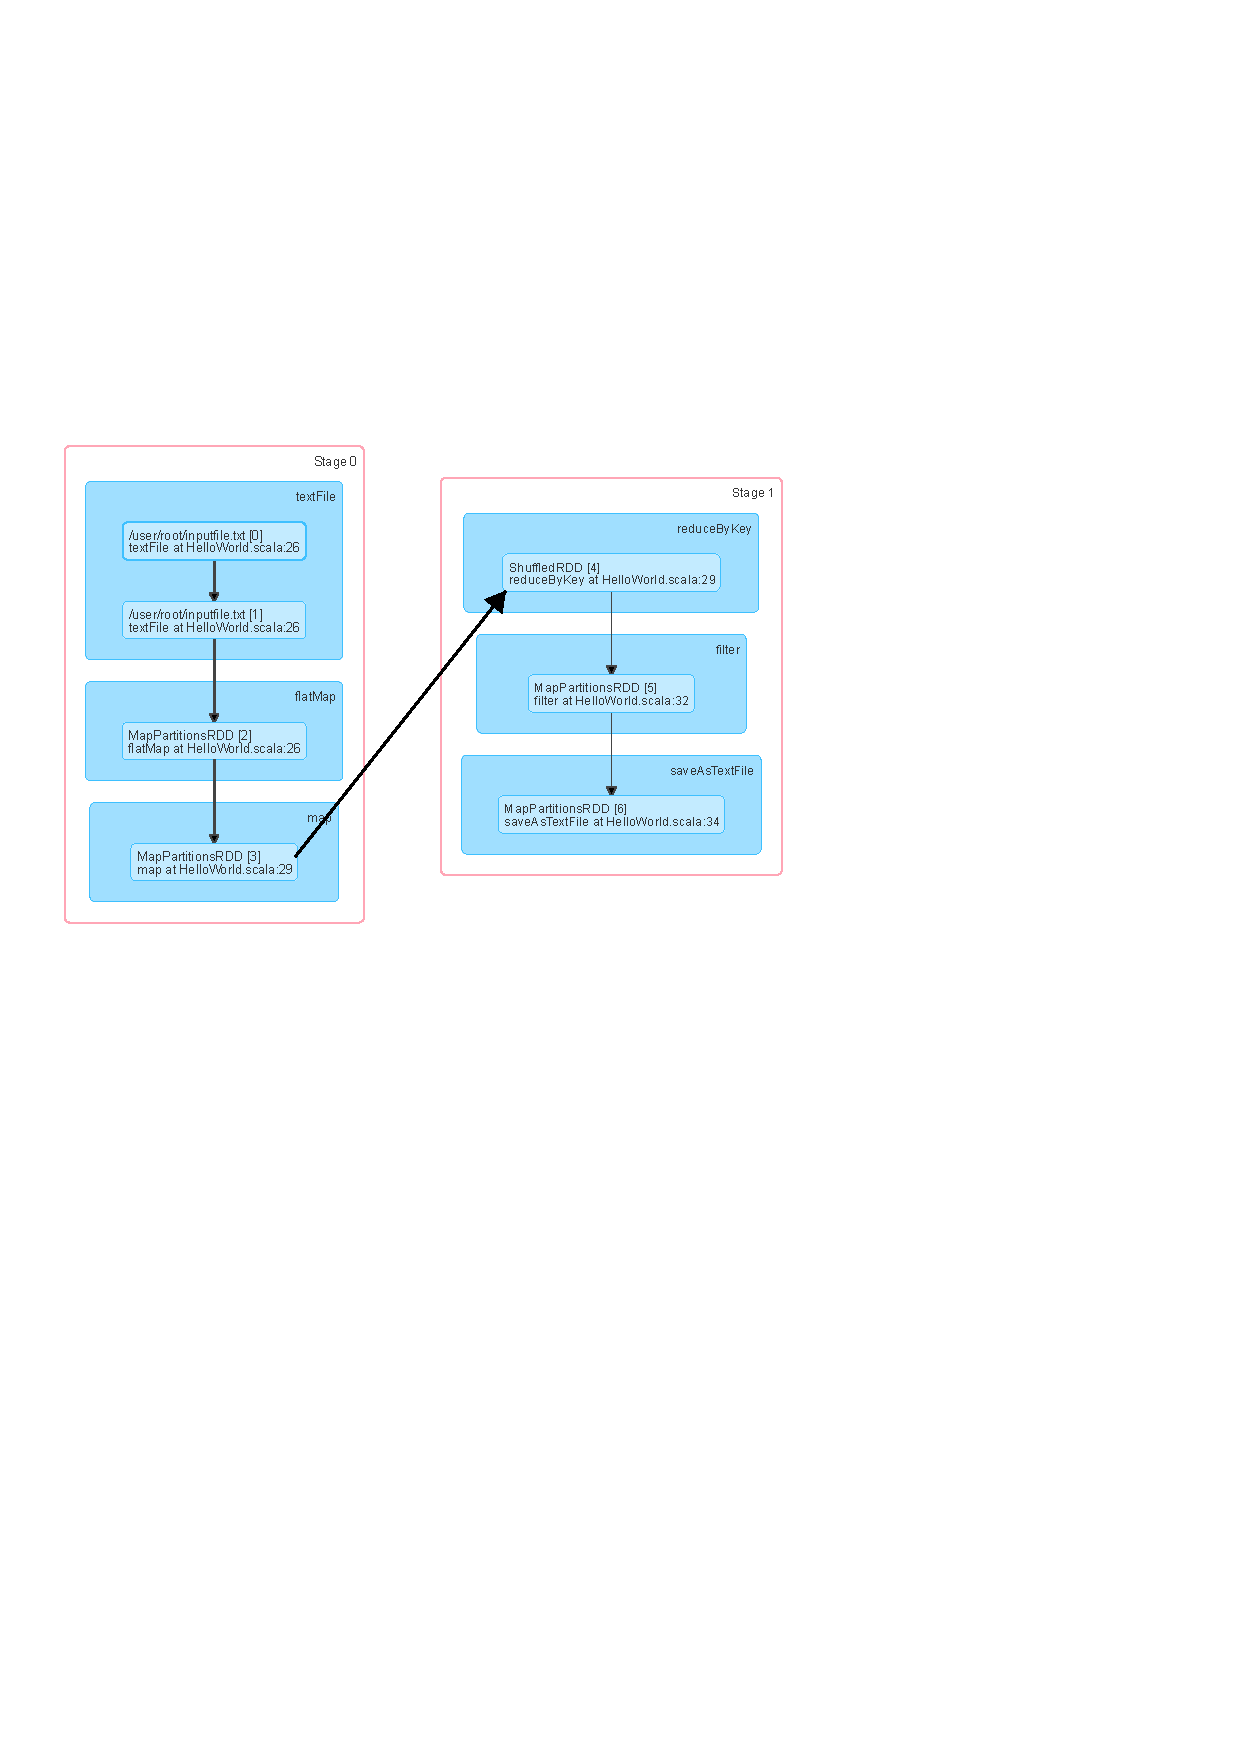
\includegraphics[width=\textwidth]{figures/SparkCountDetails.pdf}
	\caption{WordCount的RDD转换}
	\label{fig:SparkCountDetails}
\end{figure}

通过图\ref{fig:SparkCountDetails},可以清晰的看到数据被分成了两个分区,程序使用的默认分区数,即一个cpu core对应一个分区。用户对应的每一个操作会对应生成一个RDD,但对应shuffle操作如图中的reduceByKey会隐式的读在map端和reduce端分别产生一个MapPartitionRDD,中间生成一个shuffldedRDD,不过这些都是Spark内部进行的,用户不用关心。

为了加深对图\ref{fig:SparkCountDetails}中RDD的转换关系的理解,图\ref{fig:wordcountdatastream}描述了在本WordCount实例中真实数据下的转换和计算过程。
\begin{figure}[H] 
	\centering
	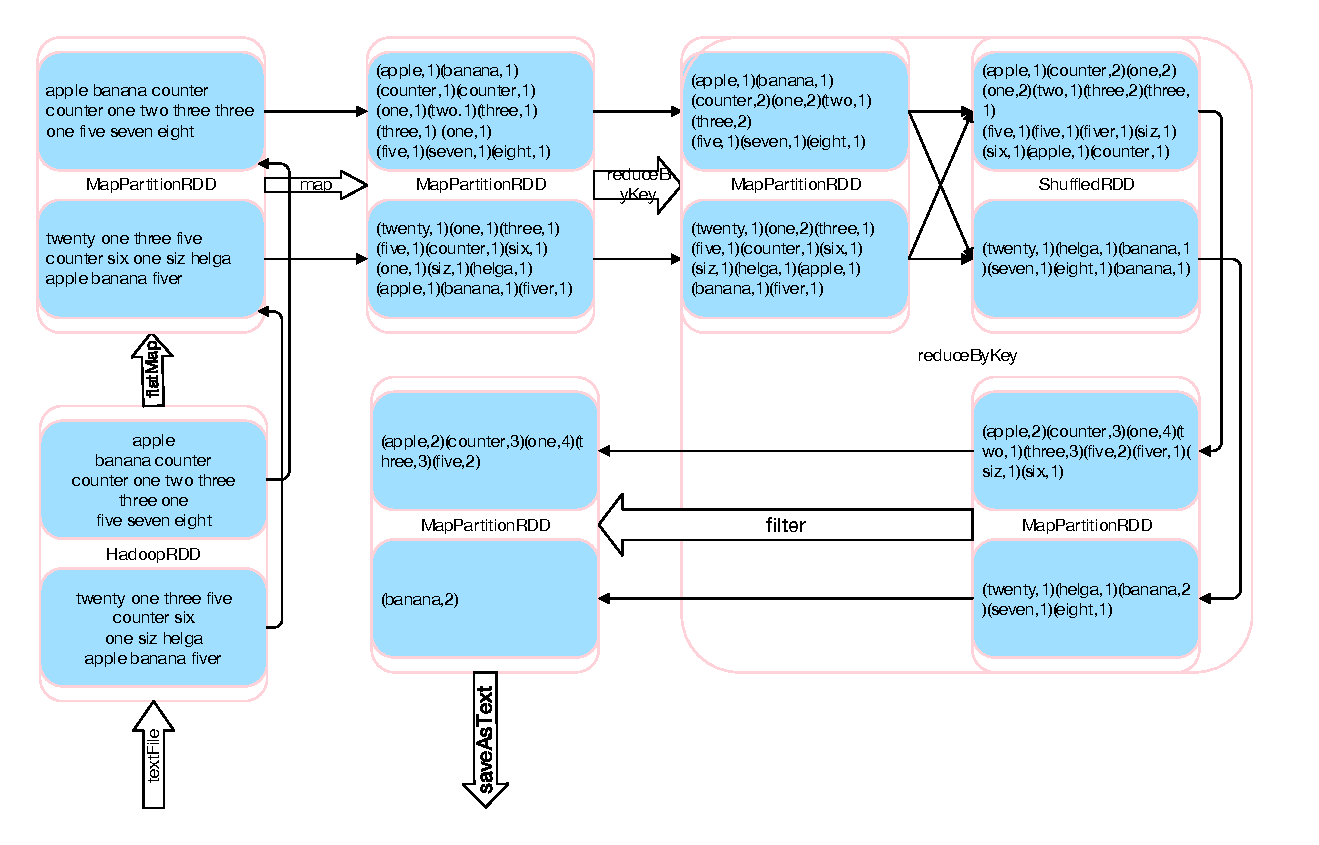
\includegraphics[width=\textwidth]{figures/wordcountdatastream.pdf}
	\caption{WordCount的数据逻辑图}
	\label{fig:wordcountdatastream}
\end{figure}

源数据存放在HDFS中,通过texFile读取后形成两个分区的HadoopRDD,这里是因为测试集群中总共两个cpu core,分区数设置为默认分区。这里也应该注意到在reduceByKey操作中,Spark产生了三个RDD,第一个为本地聚合后形成的MapPartitionRDD,第二个为通过网络操作按照分区器所设置的记录和子RDD中分区对应关系,将父RDD中相关记录拉取到子RDD中,此部分需要网络,也需要跨分区,这部分为性能调优的重点。最后一个RDD为reduce端聚合。
\chapter{Job运行和调度器模块}
\label{jobrunning}
RDD上的操作分为两种类型转换和动作。第\ref{chap:rddcreate}章中RDD的转换会构成DAG,最后RDD会触发action,WordCount例子中触发action的算子为saveAsTextFile。此算子会将数据集中的元素以textFile的形式保存到传入的路径中,本地文件或者HDFS。RDD中的saveAsTextFile经过一系列runJob的调用,最后调用了DagScheduler中的runJob。DagScheduler在第\ref{scinitial}章中已被初始化。其代码如程序\ref{inputPrg:dagrunjob}所示。
\begin{codeInput}{Scala}{DagScheduler.runJob}{dagrunjob}
def runJob[T, U](rdd: RDD[T],func: (TaskContext, Iterator[T]) => U,partitions: Seq[Int],callSite: CallSite,resultHandler: (Int, U) => Unit,properties: Properties): Unit = {
  ......
  val waiter = submitJob(rdd, func, partitions, callSite, resultHandler, properties)
  waiter.awaitResult() match {
    case JobSucceeded =>
      (waiter.jobId, callSite.shortForm, (System.nanoTime - start) / 1e9))
    case JobFailed(exception: Exception) =>
      (waiter.jobId, callSite.shortForm, (System.nanoTime - start) / 1e9))
      val callerStackTrace = Thread.currentThread().getStackTrace.tail
      exception.setStackTrace(exception.getStackTrace ++ callerStackTrace)
      throw exception
  }
}
\end{codeInput}

DagScheduler.runJobz主要调用了submitJob方法和waiter.awaitResult(),这里可以看出任务的运行是异步的。submitJob方法如程序\ref{inputPrg:submitjob}所示,代码中只保留了重要部分。
\begin{codeInput}{Scala}{DAGScheduler.submitJob}{submitjob}
def submitJob[T, U](
rdd: RDD[T],
func: (TaskContext, Iterator[T]) => U,
partitions: Seq[Int],
callSite: CallSite,
resultHandler: (Int, U) => Unit,
properties: Properties): JobWaiter[U] = {
......
val jobId = nextJobId.getAndIncrement()
......
val waiter = new JobWaiter(this, jobId, partitions.size, resultHandler)
eventProcessLoop.post(JobSubmitted(
  jobId, rdd, func2, partitions.toArray, callSite, waiter,
  SerializationUtils.clone(properties)))
  waiter
}
\end{codeInput}

由程序\ref{inputPrg:submitjob}可以看出submitJob会想生成一个jobId,并且生成jobwaiter来监听job的运行状态,最后通过DAGScheduler的事件处理线程进行处理。dag-scheduler-event-loop在SparkContex中初始化且作为守护线程存在。DAGSchedulerEventProcessLoop收到JobSubmitted事件后会立即调用DAGScheduler.handleJobSubmitted方法进行处理,这方法中会进行Stage的划分以及提交Stage。
\section{DagScheduler实现}
\subsection{Stage的划分}

在Spark中,一个Job会被分成多个Stage,各个直接存在着依赖关系,其中最下游的Stage也成为finalStage或resultStage。并行在不同分区进行相同的逻辑计算且互不影响的任务属于同一个Stage,而shuffle过程要从父RDD的多个分区中拉取数据,必须要等待多个分区任务完成才能开始计算,故其不能并行化,属于不同的Stage,DAG中划分Stage就是以Shuflle为依据进行的。

handleJobSubmitted通过调用org.apache.spark.DAGScheduler\#newResultStage来创建finalStage,
\begin{orgianlboxnotitle}
	finalStage = newResultStage(finalRDD, func, partitions, jobId, callSite)
\end{orgianlboxnotitle}

newResultStage会根据传入的finalRDD来获取父Stage和jobId,然后开始创建ResultStage即当前的Stage,这里父RDD使用列表类型。代码如程序\ref{inputPrg:newresultstage}所示
\begin{codeInput}{Scala}{DAGScheduler.newResultStage}{newresultstage}
private def newResultStage(rdd: RDD[_],func: (TaskContext, Iterator[_]) => _,partitions: Array[Int],
jobId: Int,callSite: CallSite): ResultStage = {
  val (parentStages: List[Stage], id: Int) = getParentStagesAndId(rdd, jobId)
  val stage = new ResultStage(id, rdd, func, partitions, parentStages, jobId, callSite)
  stageIdToStage(id) = stage
  updateJobIdStageIdMaps(jobId, stage)
  stage
}
\end{codeInput}

程序\ref{inputPrg:newresultstage}中getParentStagesAndId方法会进一步调用getParentStages方法,getParentStages方法为划分Stage的核心。它的返回类型为List[Stage],每遇到DAG中RDD的ShuffleDependency就会参数一个新的Stage,其代码如程序\ref{inputPrg:getparentstages}所示。
\begin{codeInput}{Scala}{DAGScheduler.getParentStages}{getparentstages}
private def getParentStages(rdd: RDD[_], firstJobId: Int): List[Stage] = {
  val parents = new HashSet[Stage]
  val visited = new HashSet[RDD[_]]
  val waitingForVisit = new Stack[RDD[_]]
  def visit(r: RDD[_]) {
    if (!visited(r)) {
      visited += r
      for (dep <- r.dependencies) {
        dep match {
          case shufDep: ShuffleDependency[_, _, _] =>
            parents += getShuffleMapStage(shufDep, firstJobId)
          case _ =>waitingForVisit.push(dep.rdd)
        }
      }
    }
  }
  waitingForVisit.push(rdd)
  while (waitingForVisit.nonEmpty) {
    visit(waitingForVisit.pop())
  }
  parents.toList
}
\end{codeInput}

getParentStages方法中定义了一个visit方法,此方法会对方法外的变量parents、visited及waitingForVisit产生影响,这里用到Scala函数的闭包特性。getParentStages变量说明如下
\begin{centertitlebox}{getParentStages变量说明}
	parents:存放各个ShuffleDependency所依赖的Stage\\
	visited:存放DAG中已经遍历过的RDD\\
	waitingForVisit:存放即将要遍历的RDD,为栈结构
\end{centertitlebox}
\subsection{实例:WordCount划分Stage}

以本WordCount样例展示如何划分Stage。WordCount DAG如图\ref{fig:SparkCountDetails}所示,提前三个重要的信息组成新的RDD数据结构,定义如下
\begin{centertitlebox}{新定义RDD数据结构}
	数据结构:RDD(deps:List[Dependency],partitions:List(partitionId))\\
	deps:代表当前RDD的依赖列表\\
	partitions:指当前RDD的分区列表\\
	textFile:\\  HadoopRDD[1](Nil,List(1,2))\\
	flatMap:\\  MapPartitionRDD[2](List(onoToOneDependency(HadoopRDD[1]),List(1,2))\\
	map:\\  MapPartitionRDD[3](List(onoToOneDependency(MapPartitionRDD[2])),List(1,2))\\
	reduceByKey:\\  ShuffledRDD[4](List(ShuffleDependency(MapPartitionRDD[3])),List(3,4))\\
	filter:\\  MapPartitionRDD[5](List(onoToOneDependency(ShuffledRDD[4])),List(3,4))\\
	saveTextFile:\\  MapPartitionRDD[6](List(onoToOneDependency(MapPartitionRDD[5])),List(3,4))
\end{centertitlebox}

这里定义RDD中包含了两种数据元素,分别为当前RDD的依赖列表和当前RDD的分区列表。依赖列表中存放有当前RDD所依赖的父RDD的对象,分区列表中存放着分区的Id,要获取该分区数据可以通过BlockManager来获取。

DAG以finalRDD即MapPartitionRDD[6]为起始点,依次进入函数getParentStages,各变量参数的值变化情况如表\ref{tab:getstage}所示
\begin{table}[H]
	\caption{getParentStages变量值}
	\label{tab:getstage}
	\begin{tabularx}{\linewidth}{lXX}
		\toprule[1.5pt]
		{\heiti visited:HashSet} & {\heiti parents:HashSet} &{\heiti waittingForVisit:Stack}\\
		\midrule[1pt]
		6& Nil &6 \\
		6& Nil &5 \\
		6 5& Nil &4 \\
		6 5 4& ShuffleMapStage(3,shuffleDep(3)) &Nil \\
		\bottomrule[1.5pt]
	\end{tabularx}
\end{table}

这里函数生成了ShuffleMapStage,其中存放了RDD[3]的信息,另外ShuffleMapStage中Task计算的结果会传给Driver端的mapOutputTracker,其他任Task可以通过查询它来获取这些结果,不过这些结果并不是真实的数据,而是保存真实数据所在位置、大小等元数据信息,其他Task通过这些元数据信息获取其需要处理的数据。接下来回到程序\ref{inputPrg:newresultstage},进入newResultStage代码块。最后返回ResultStage(RDD[6],List(ShuffleMapStage(3,shuffleDep(3))))。最后函数newResultStage将jobId和ResultStage进行绑定,返回ResultStage,也就是finalStage。
\section{任务调度器实现}
\subsection{任务的生成}

现在回到handleJobSubmitted,上节生成了finalStage,此方法后面部分会调用submitStage来提交这个Stage,如果当前提交的Stage还有父Stage没有提交,那么就递归提交父Stage,只有父Stage提交完了,才能提交当前Stage,submitStage如程序\ref{inputPrg:submitStage}所示
\begin{codeInput}{Scala}{DAGScheduler.submitStage}{submitStage}
private def submitStage(stage: Stage) {
  val jobId = activeJobForStage(stage)
  if (jobId.isDefined) {
    if (!waitingStages(stage) && !runningStages(stage) && !failedStages(stage)) {
      val missing = getMissingParentStages(stage).sortBy(_.id) //List(ShuffleMapStage[0])
      if (missing.isEmpty) {
        submitMissingTasks(stage, jobId.get)
      } else {
        for (parent <- missing) {
          submitStage(parent)
        }
        waitingStages += stage//此时waitingStages=set(ResultStage 1)
      }
    }
  } else {
    abortStage(stage, "No active job for stage " + stage.id, None)
  }
}
\end{codeInput}

经过上节DAGScheduler对DAG Stage的划分,WordCount实例逻辑上可以形成图\ref{fig:SparkCountDetails}所示的Stage。Stage1作为submitStage的参数进入,函数先判断其是否有父Stage,有父Stage就递归提交父Stage,最后会由submitMissingTasks来完成最后的提交任务工作。submitMissingTasks函数会首先分析其包含的分区数,对于每一个分区会为其生成一个Task,然后同属于一个Stage的Task会被封装为TaskSet,最后提交给TaskScheduler。TaskSet中包含了一组处理逻辑完全相同的Task,只是作用数据不同。
\subsection{TaskScheduler的创建}

对于每个TaskScheduler都会对应一个SchedulerBackend。其中TaskScheduler负责程序的不同job之间的调度,SchedulerBackend负责与集群资源管理器进行通信,取得应用所需要的资源,并且将资源传递给TaskScheduler,由TaskScheduler为其最后分配计算资源。

TaskScheduler和SchedulerBackend在SparkContext初始化的时候创建,不同的资源管理模式和部署模式下其对应的值不相同,在SparkContext初始化章节中分析了Yarn-Cluster模式下TaskScheduler和SchedulerBackend分别对应YarnClusterScheduler和YarnClusterSchedulerBackend。这里TaskScheduler和SchedulerBackend都是接口,SchedulerBackend负责分配当前可用的资源,具体就是向当前等待分配计算资源的Task分配计算资源。

\subsection{Task的提交}

submitMissingTasks中会通过TaskScheduler.submitTasks来提交Tasks,TaskScheduler提供的是一个接口,在不同模式下会有不同实现。在Yarn-Cluster模式下会调用TaskSchedulerImpl.submitTasks(TaskSet),其作用首先将保存这组任务的TaskSet加入到一个TaskManager中,TaskManager会根据数据的locality aware为Task分配资源,并且也对Task的执行状态监控。接着为应用分配调度策略,主要包括FIFO和FAIR。默认情况下为FIFO,调度的单位为TaskSet,优先调度jobId小的以及先到rootPool的TaskSet。最后将调用SchedulerBackend.reviveOffers(),实际调用CoarseGrainedSchedulerBackend.reviveOffers(),接着调用CoarseGrainedSchedulerBackend.DriverEndpoint.makeOffers(),遍历出每个Executor的资源封装之后,传入TaskSchlerImpl.resourceOffers()为每个Task分配具体的Executor,分配资源部分代码如程序\ref{inputPrg:allocateRes}所示
\begin{codeInput}{Scala}{TaskSchedulerImpl.resourceOffers}{allocateRes}
//为了避免Task集中分配到某些机器上,随机打乱
val shuffledOffers = Random.shuffle(offers)
//存储分配好的Task
val tasks = shuffledOffers.map(o => new ArrayBuffer[TaskDescription](o.cores))
val availableCpus = shuffledOffers.map(o => o.cores).toArray
val sortedTaskSets = rootPool.getSortedTaskSetQueue
for (taskSet <- sortedTaskSets) {
  taskSet.parent.name, taskSet.name, taskSet.runningTasks))
  if (newExecAvail) {
    taskSet.executorAdded()
  }
}
var launchedTask = false
for (taskSet <- sortedTaskSets; maxLocality <- taskSet.myLocalityLevels) {
  do {
    launchedTask = resourceOfferSingleTaskSet(taskSet, maxLocality, shuffledOffers, availableCpus, tasks)
  } while (launchedTask)
}
if (tasks.size > 0) {
  hasLaunchedTask = true
}
return tasks
\end{codeInput}

程序返回的是TaskDescription的二维数组,TaskDescription包含的是TaskId、ExecutorId和Task执行所需要的依赖环境信息等。

最后调用CoarseGrainedSchedulerBackend.DriverEndPoint.launchTasks,它的输入为一个TaskDescription的二维数组,即上面程序段的返回值。此函数的作用先对TaskDescription进行序列化,然后更新Executor资源状况,空闲cpu core减去每个Task需要的cpu core,最后将Task通过Rpc发送到Executor,Executor收到这个消息后就会开始执行Task。相应的代码如程序\ref{inputPrg:driverlaunchtasks}所示
\begin{codeInput}{Scala}{CoarseGrainedSchedulerBackend.DriverEndPoint.launchTasks}{driverlaunchtasks}
private def launchTasks(tasks: Seq[Seq[TaskDescription]]) {
  for (task <- tasks.flatten) {
  val serializedTask = ser.serialize(task)
  if (serializedTask.limit >= akkaFrameSize - AkkaUtils.reservedSizeBytes) {
    scheduler.taskIdToTaskSetManager.get(task.taskId).foreach { taskSetMgr =>
    try {
      taskSetMgr.abort(msg)
    } catch {
      case e: Exception => logError("Exception in error callback", e)
    }
  }
  }
  else {
    val executorData = executorDataMap(task.executorId)
    executorData.freeCores -= scheduler.CPUS_PER_TASK
    executorData.executorEndpoint.send(LaunchTask(new SerializableBuffer(serializedTask)))
    }
  }
}
\end{codeInput}

Executor执行Task会在下一章中进行介绍。
\subsection{Task计算结果的处理}
\label{driverdealresult}
Executor在执行完Task时会向Driver发送StatusUpdate的消息来通知Driver任务的状态更新未TaskState.FINISHED。Driver会通知TaskScheduler,TaskScheduler会执行TaskSchedulerImpl.statusUpdate,其代码如程序\ref{inputPrg:taskimplstatus}所示
\begin{codeInput}{Scala}{TaskSchedulerImpl.statusUpdate}{taskimplstatus}
taskIdToTaskSetManager.get(tid) match {
  case Some(taskSet) => 
    if (TaskState.isFinished(state)) {
    taskIdToTaskSetManager.remove(tid)
    taskIdToExecutorId.remove(tid).foreach { execId =>
      if (executorIdToTaskCount.contains(execId)) {
        executorIdToTaskCount(execId) -= 1
     }
    }
  }
  if (state == TaskState.FINISHED) {
    taskSet.removeRunningTask(tid)
    taskResultGetter.enqueueSuccessfulTask(taskSet, tid, serializedData)
  } else if (Set(TaskState.FAILED, TaskState.KILLED, TaskState.LOST).contains(state)) {
    taskSet.removeRunningTask(tid)
    taskResultGetter.enqueueFailedTask(taskSet, tid, state, serializedData)
  }
  case None =>
    logError(
    ("Ignoring update with state %s for TID %s because its task set is gone (this is " +
    "likely the result of receiving duplicate task finished status updates)")
    .format(state, tid))
}
\end{codeInput}

Task只有在FINISHED状态下,才会被标记为成功,其他状态为执行失败。对于成功的Task,Driver会将Task加入到成功任务队列。Executor执行Task成功返回的结果可能有两种情形,
\begin{enumerate}[\bfseries 1]
    \item 直接结果
    
    这种情况下直接返回结果即可
    \item 非直接结果
    
    需要向远程worker网络获取结果,获取之后在远程节点上删除结果,这通过Spark中的BlockManager完成。
\end{enumerate}

这两种结果的产生会在下章Executor执行Task章节讲述。

接着通过TaskScheduleImpl.handleSuccessfulTask来负责处理获取到的计算结果。这里调用栈如下所示
\begin{centertitlebox}{handleSuccessfulTask调用栈}
	(1)TaskScheduleImpl.handleSuccessfulTask\\
	(2)TaskSetManager.handleSuccessfulTask\\
	(3)DAGScheduler.taskEnded\\
	(4)DAGScheduler.handleTaskCompletion
\end{centertitlebox}

其中最核心的为第4个,它会对不同的Task进行模式匹配,进行不同的处理,对于ShuffleMapTask,程序代码如程序\ref{inputPrg:shufflemaptask}所示
\begin{codeInput}{Scala}{ShuffleMapTask结果处理}{shufflemaptask}
case smt: ShuffleMapTask =>
  val shuffleStage = stage.asInstanceOf[ShuffleMapStage]
  updateAccumulators(event)
  val status = event.result.asInstanceOf[MapStatus]
  val execId = status.location.executorId
  if (failedEpoch.contains(execId) && smt.epoch <= failedEpoch(execId)) {
  } else {
    shuffleStage.addOutputLoc(smt.partitionId, status)
  }
  if (runningStages.contains(shuffleStage) && shuffleStage.pendingPartitions.isEmpty) {
    markStageAsFinished(shuffleStage)
    mapOutputTracker.registerMapOutputs(
    shuffleStage.shuffleDep.shuffleId,
    shuffleStage.outputLocInMapOutputTrackerFormat(),
    changeEpoch = true)	
    clearCacheLocs()	
    if (!shuffleStage.isAvailable) {
      shuffleStage.findMissingPartitions().mkString(", "))
      submitStage(shuffleStage)
    } else {
      if (shuffleStage.mapStageJobs.nonEmpty) {
        val stats = mapOutputTracker.getStatistics(shuffleStage.shuffleDep)
        for (job <- shuffleStage.mapStageJobs) {
          markMapStageJobAsFinished(job, stats)
        }
      }
    }
}
\end{codeInput}

首先会将整体结果注册到MapOutputTracker中去,这样下一个Stage的Task就可以方便的获取所需数据的元数据信息。接着判断当前Stage中是否所有任务都已成功返回,如果有部分数据是空的,那证明执行该分区的Task执行失败,需要重新提交Stage;如果当前Stage执行成功并且没有父Stage,那么就通过submitWaitingStages()将waitingStage集合中的Stage提交。

至此一个Stage就已经执行完成,如果Stage是ResultStage,那么一个job就执行完成了。

Spark中有两种Task,ShuffleMapTask和ResultTask。ShuffleMapTask根据Task的Partition存放计算结果,而ResultTask将计算结果发送到Driver。用户程序出发action后,会调用SparkContext的runJob方法开始进行任务的提交。最后会通过DAG的事件处理器传递到DAGScheduler.handleJobSubmitted,它会首先划分Stage,然后提交Task。至此,Task开始在集群上运行了。
Stage的开始就是从外部存储或者shuffle结果中读取数据;一个Stage的结束就是由于发生shuflle或者生成结果。

\chapter{Executor执行Task}
\section{Executor启动}

Yarn-Cluster模式下AM中SparkContext初始化完成之后,AM就开始在集群中划分资源,启动container。

AM通过循环等待spark.yarn.am.waitTime中定义的时间监听SparkContext的初始化状态,最后获得SparkContext的初始化实例。如果初始化实例为空,则报错并将应用状态置为失败。SparkContext不为空的情况下,将会注册AM。注册AM核心代码如程序\ref{inputPrg:registeram}所示
\begin{codeInput}{Scala}{Driver端am注册}{registeram}
allocator = client.register(driverUrl,
driverRef,
yarnConf,
_sparkConf,
uiAddress,
historyAddress,
securityMgr)
allocator.allocateResources()
reporterThread = launchReporterThread()
\end{codeInput}

程序\ref{inputPrg:registeram}中client其实为YarnRMClient,是与RM\footnote{RM为ResourceManager的简称,以后提到RM均为ResourceManage}负责通信的。client.register的作用就是向RM中注册AM,并获得YarnAllocator实例对象,此对象的作用体现在下一行代码。

程序的调用栈如下所示
\begin{orgianlboxnotitle}
	(1)YarnAllocator\#allocateResources()\\
	(2)YarnAllocator\#handleAllocatedContainers\\
	(3)YarnAllocator\#runAllocatedContainers
\end{orgianlboxnotitle}

调用栈(1)负责和RM通信确保资源能够满足请求的资源,如果满足将会生成和请求资源最大Executor数量相等的Container。调用栈(2)将会匹配RM所提供的Container,并决定在其上启动Executor。调用栈(3)是负责启动的模块,也是本程序的重点,其代码段如程序\ref{inputPrg:runContainer}所示,流程图如图\ref{fig:runContainer}所示。
\begin{figure}[H] 
	\centering
	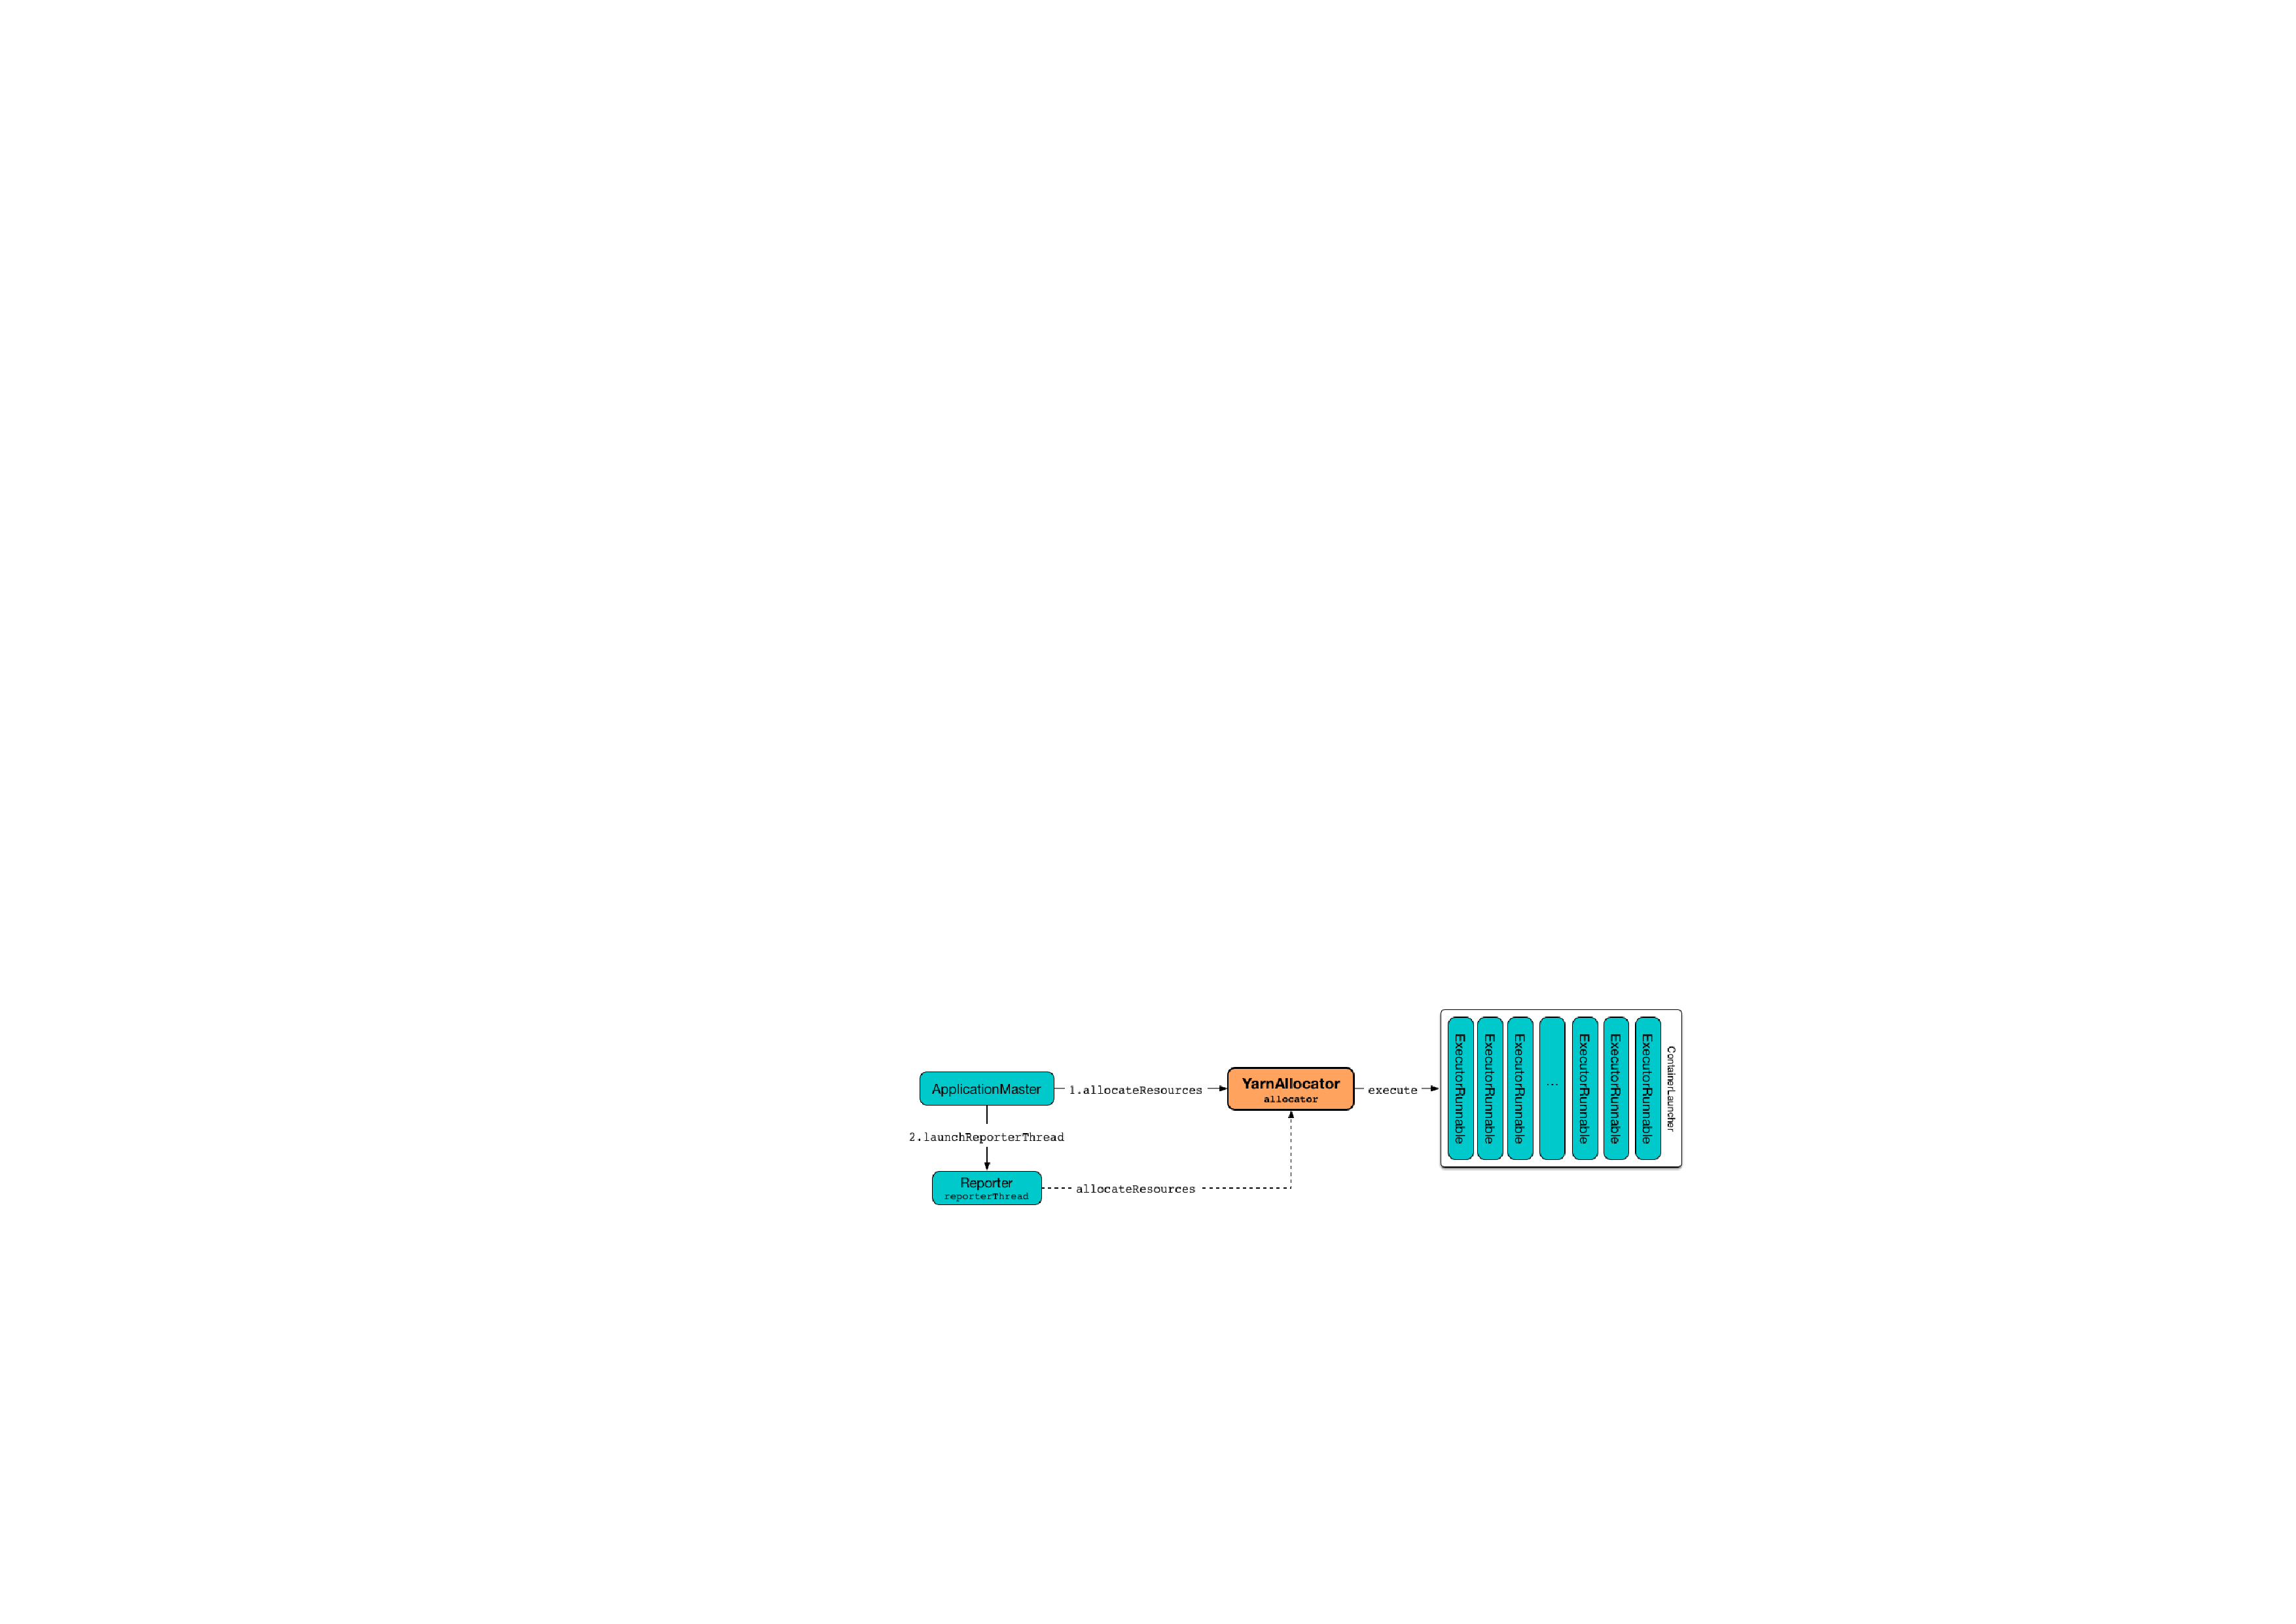
\includegraphics[width=\textwidth]{figures/YarnAllocator.pdf}
	\caption{YarnAllocator启动Container流程}
	\label{fig:runContainer}
\end{figure}
\begin{codeInput}{Scala}{启动Executor}{runContainer}
for (container <- containersToUse) {
  numExecutorsRunning += 1
  val executorHostname = container.getNodeId.getHost
  val containerId = container.getId
  executorIdCounter += 1
  val executorId = executorIdCounter.toString
  executorIdToContainer(executorId) = container
  containerIdToExecutorId(container.getId) = executorId	
  val containerSet = allocatedHostToContainersMap.getOrElseUpdate(executorHostname,
    new HashSet[ContainerId])	
  containerSet += containerId
  allocatedContainerToHostMap.put(containerId, executorHostname)	
  val executorRunnable = new ExecutorRunnable(container,conf,sparkConf,driverUrl,executorId,
  executorHostname,executorMemory,executorCores,
  appAttemptId.getApplicationId.toString,securityMgr)
  if (launchContainers) {
    launcherPool.execute(executorRunnable)
  }
}
\end{codeInput}

targetNumExecutors为Executor的总数,默认情况为2,当用户没有开启动态分配并手动指定targetNumExecutors的数量时,系统会逐个Executor分配Container。同时会将生成的Executor标识唯一的ID,且与Container进行绑定,最后会通过ExecutorRunnable实例的run方法到NM\footnote{NM为NodeManager的简称,以后提到NM均为NodeManage}中启动Container。每个Container中包含了Executor的核数和内存大小,通过Java命令启动Executor实例即CoarseGrainedExecutorBackend。CoarseGrainedExecutorBackend的main方法首先会对启动它时传来的参数进行解析,只会会调用run方法,代码细节如程序\ref{inputPrg:executorBackendRun}所示
\begin{codeInput}{Scala}{CoarseGrainedExecutorBackend.run}{executorBackendRun}
SignalLogger.register(log)
SparkHadoopUtil.get.runAsSparkUser { () =>
  val executorConf = new SparkConf
  val port = executorConf.getInt("spark.executor.port", 0)
  //这个fetcher通过rpcenv用来获得driver的ref,之后就关闭了
  val fetcher = RpcEnv.create("driverPropsFetcher",hostname,port,
  executorConf,new SecurityManager(executorConf),clientMode = true)
  val driver = fetcher.setupEndpointRefByURI(driverUrl)
  //获得Driver端的配置信息
  val props = driver.askWithRetry[Seq[(String, String)]](RetrieveSparkProps) ++
  Seq[(String, String)](("spark.app.id", appId))
  fetcher.shutdown()	
  // 使用从Driver端获取的配置信息创建SparkEnv
  val driverConf = new SparkConf()
    for ((key, value) <- props) {
      if (SparkConf.isExecutorStartupConf(key)) {
        driverConf.setIfMissing(key, value)
      } else {
        driverConf.set(key, value)
      }
    }
  //这里如果是yarn模式下,他其实一直在跟新和HDFS交互的密钥信息
  if (driverConf.contains("spark.yarn.credentials.file")) {
    SparkHadoopUtil.get.startExecutorDelegationTokenRenewer(driverConf)
  }
  //创建ExecutorEnv,代码和Driver端的基本一摸一样
  val env = SparkEnv.createExecutorEnv(driverConf, executorId, hostname, port, cores, isLocal = false)	
  val sparkHostPort = env.conf.getOption("spark.executor.port").map { port =>
    hostname + ":" + port}.orNull
  //这里创建了一个Endpoint用于与driver交互执行task。是由此可以看出Executor的真正实现CoarseGrainedExecutorBackend
  env.rpcEnv.setupEndpoint("Executor", new CoarseGrainedExecutorBackend(
  env.rpcEnv, driverUrl, executorId, sparkHostPort, cores, userClassPath, env))
  //WorkerWatcher就是用来监视worker的,当与worker断开连接时,它将会关闭这个jvm进程
  workerUrl.foreach { url =>
    env.rpcEnv.setupEndpoint("WorkerWatcher", new WorkerWatcher(env.rpcEnv, url))
  }
  env.rpcEnv.awaitTermination()
  SparkHadoopUtil.get.stopExecutorDelegationTokenRenewer()
}
\end{codeInput}

Executor创建于Driver交互的RPC环境后,会立刻执行CoarseGrainedExecutorBackend的onStart()方法,该方法最重要的作用是向Driver注册Executor的信息,主要为executorId和cores等。注册的消息会在CoarseGrainedSchedulerBackend\#receiveAndReply中接收,在Driver端会通过executorDataMap(HashMap[String,ExecutorData])数据结构进行存储,TaskScheduler对将task封装为TaskDescription时会用到executorDataMap中的信息。
\section{Task的执行}

第\ref{jobrunning}章Driver通过CoarseGrainedSchedulerBackend.DriverEndPoint.launchTasks会将Task分配到Executor上,这里通过的是nettyRpc。

CoarseGrainedExecutorBackend收到LaunchTask消息后,会调用Executor的launchTask启动Task,如程序\ref{inputPrg:executorlaunchtask}
\begin{codeInput}{Scala}{CoarseGrainedExecutorBackend消息处理模块}{executorlaunchtask}
case LaunchTask(data) =>
  if (executor == null) {
    logError("Received LaunchTask command but executor was null")
    System.exit(1)
  } else {
    val taskDesc = ser.deserialize[TaskDescription](data.value)
    logInfo("Got assigned task " + taskDesc.taskId)
    executor.launchTask(this, taskId = taskDesc.taskId, attemptNumber = taskDesc.attemptNumber,
    taskDesc.name, taskDesc.serializedTask)
}
\end{codeInput}

Executor.launchTask方法如程序块\ref{inputPrg:executorrunner}所示
\begin{codeInput}{Scala}{Executor.launcherTask}{executorrunner}
val tr = new TaskRunner(context, taskId = taskId, attemptNumber = attemptNumber, taskName,
serializedTask)
runningTasks.put(taskId, tr)
threadPool.execute(tr)
\end{codeInput}

Executor会输入的Task生成一个TaskRunner,最终会被放到一个ThreadPool中去。TaskRunner为一个线程,重写其run方法,run中会执行Task。

\subsection{Task执行前的准备}

Driver端生成Task的时候会将Task依赖的文件和jar信息都封装到Task中去,在Executor端,得先恢复这些信息。
\begin{orgianlboxnotitle}
  val (taskFiles,taskJars,taskBytes) = Task.deserializeWithDependencies(serializedTask)\\
  updateDependencies(taskFiles, taskJars)
\end{orgianlboxnotitle}

这里返回了三元组,信息包含了taskFiles、taskJars和taskBytes,这些信息只是属于类似于元数据的信息,接下来Executor还需要调用updateDependencies下载这些依赖:
\begin{orgianlboxnotitle}
// Fetch file with useCache mode, close cache for local mode.\\
Utils.fetchFile(name, new File(SparkFiles.getRootDirectory()), conf,\\
env.securityManager, hadoopConf, timestamp, useCache = !isLocal)
\end{orgianlboxnotitle}

依赖下载完成后,Executor会通过TaskRunner来执行Task。
\subsection{执行Task}

准备工作做好后,Executor就是执行Task.run方法来运行Task,如程序\ref{inputPrg:executorruntask}所示
\begin{codeInput}{Scala}{Execotor执行Task}{executorruntask}
//开始执行Task
taskStart = System.currentTimeMillis()
var threwException = true
val (value, accumUpdates) = try {
  val res = task.run(
  taskAttemptId = taskId,
  attemptNumber = attemptNumber,
  metricsSystem = env.metricsSystem)
  threwException = false
  res
} finally {
  ......
}
val taskFinish = System.currentTimeMillis()
\end{codeInput}

程序\ref{inputPrg:executorruntask}中task.runTask会调用Task.run方法,此方法为final类型,首先会本次Task生成TaskContext,也就是保留本Task的上下文信息。最后TaskContext还会在Task执行完成后对次Task标记成功并通过回调函数来完成最终的处理,如程序\ref{inputPrg:marktaskcomplete}所示
\begin{codeInput}{Scala}{TaskContext任务成功时执行回调}{marktaskcomplete}
private[spark] def markTaskCompleted(): Unit = {
  completed = true
  val errorMsgs = new ArrayBuffer[String](2)
  onCompleteCallbacks.reverse.foreach { listener =>
  try {
    listener.onTaskCompletion(this)
  } catch {
    case e: Throwable =>
      errorMsgs += e.getMessage
    }
  }
  if (errorMsgs.nonEmpty) {
    throw new TaskCompletionListenerException(errorMsgs)
  }
}
\end{codeInput}

整个Task.run的核心程序如\ref{inputPrg:taskrun}所示
\begin{codeInput}{Scala}{Task run方法核心部分}{taskrun}
//设置上下文信息,实际上会调用org.apache.spark.TaskContext#setTaskContext
TaskContext.setTaskContext(context)
//更新metrics信息
context.taskMetrics.setHostname(Utils.localHostName())
context.taskMetrics.setAccumulatorsUpdater(context.collectInternalAccumulators)
//当前线程,在被打断的时候可以通过它来停止该线程
taskThread = Thread.currentThread()
if (_killed) {//如果当前Task被杀死,那么需要退出Task的执行
  kill(interruptThread = false)
}
try {
  //执行本次Task,runTask真正执行代码为子类中重写的runTask,对应ShuffleMapTask和ResultTask
  (runTask(context), context.collectAccumulators())
} catch {
} finally {
  // Call the task completion callbacks.
  context.markTaskCompleted()
  try {
  }
  } finally {
    TaskContext.unset()
  }
}
\end{codeInput}

这里的runTask会有两种不同的实现方法,分别为ShuffleMapTask和ResultTask,两种Task前期阶段处理基本相同,如程序\ref{inputPrg:common}所示。
\begin{codeInput}{Scala}{两种Task共同的处理方式}{common}
// Deserialize the RDD using the broadcast variable.
val deserializeStartTime = System.currentTimeMillis()
//获取反序列化实例
val ser = SparkEnv.get.closureSerializer.newInstance()
//以下两端代码是其区别,上面的为ShuffleMapTask,下面为ResultTask
val (rdd, dep) = ser.deserialize[(RDD[_], ShuffleDependency[_, _, _])](
//获取rdd和作用于rdd结果的函数
val (rdd, func) = ser.deserialize[(RDD[T], (TaskContext, Iterator[T]) => U)](

ByteBuffer.wrap(taskBinary.value), Thread.currentThread.getContextClassLoader)
_executorDeserializeTime = System.currentTimeMillis() - deserializeStartTime
//Task的测量信息
metrics = Some(context.taskMetrics)
\end{codeInput}
\begin{enumerate}[\bfseries 1]
	\item 对于ShuffleMapTask
	
	ShuffleMapTask是根据Stage中分区数量来生成的,它会根据该Stage每个RDD连接操作作用于对应的partition上,并将结果生成文件供下游Task使用。ShuffleMapTask核心代码段如程序\ref{inputPrg:shufflemaptask}所示
\begin{codeInput}{Scala}{ShuffleMapTask核心部分实现分析}{shufflemaptask}
//从SparkEnv中获得shuffleManager,具体分析会在shuffle模块讲述
val manager = SparkEnv.get.shuffleManager
//从shuffleManager获得写入器
writer = manager.getWriter[Any, Any](dep.shuffleHandle, partitionId, context)
//调用rdd开始计算,并且最后通过写入器写入文件系统
writer.write(rdd.iterator(partition, context).asInstanceOf[Iterator[_ <: Product2[Any, Any]]])
//关闭写入器,并将最后结果返回
writer.stop(success = true).get
\end{codeInput}
	\item 对于ResultTask
	
	ResultStage会根据生成结果的Partition来生成与Partition数量相同的ResultTask,最后会将计算结果回传给Driver端,这里的结果不一定是真实的数据。ResultTask的作用代码如程序\ref{inputPrg:ResultTask}所示。
\begin{codeInput}{Scala}{ResultTask核心部分实现分析}{ResultTask}
//调用rdd的迭代器执行传入函数的操作
func(context, rdd.iterator(partition, context))
\end{codeInput}
\end{enumerate}

\subsection{Task结果的处理}
Executor运行完Task后,就会将结果保存在DirectTaskResult里,如程序\ref{inputPrg:executorresult}所示
\begin{codeInput}{Scala}{Executor对Task结果的处理}{executorresult}
//任务运行结果的处理
val resultSer = env.serializer.newInstance()
val beforeSerialization = System.currentTimeMillis()
//value中保存Task的计算结果
val valueBytes = resultSer.serialize(value)
val afterSerialization = System.currentTimeMillis()
//首先将结果直接放入org.apache.spark.scheduler.DirectTaskResult
val directResult = new DirectTaskResult(valueBytes, accumUpdates, task.metrics.orNull)
val serializedDirectResult = ser.serialize(directResult)
val resultSize = serializedDirectResult.limit
\end{codeInput}

但是serializedDirectResult并不是直接回传给Driver,Executor通过程序\ref{inputPrg:executorsendresult}的策略对结果进行不同处理。
\begin{codeInput}{Scala}{Executor回传结果策略}{executorsendresult}
// directSend = sending directly back to the driver
val serializedResult: ByteBuffer = {
if (maxResultSize > 0 && resultSize > maxResultSize) {
  //如果resultSize大于spark.drive.driver.maxResultSize设置的大小值,则直接丢弃
  ser.serialize(new IndirectTaskResult[Any](TaskResultBlockId(taskId), resultSize))
} else if (resultSize >= akkaFrameSize - AkkaUtils.reservedSizeBytes) {
  //如果不能通过AKKA的消息传递,那么放入BlockManager等待调用者以网络形式来获取
  //AKKA的消息默认大小可以通过spark.akka.frameSize来设置
  val blockId = TaskResultBlockId(taskId)
  env.blockManager.putBytes(
  blockId, serializedDirectResult, StorageLevel.MEMORY_AND_DISK_SER)
  ser.serialize(new IndirectTaskResult[Any](blockId, resultSize))
} else {
  //结果回传Driver
  serializedDirectResult
 }
}
//通过AKKA向driver汇报本次Task已经完成
execBackend.statusUpdate(taskId, TaskState.FINISHED, serializedResult)
\end{codeInput}

而execBackend.statusUpdate实际上调用的CoarseGrainedExecutorBackend.statusUpdate,程序如\ref{inputPrg:execbankendstatus}所示
\begin{codeInput}{Scala}{Executor执行回传消息}{execbankendstatus}
val msg = StatusUpdate(executorId, taskId, state, data)
driver match {
  case Some(driverRef) => driverRef.send(msg)
  case None => logWarning(s"Drop $msg because has not yet connected to driver")
}
\end{codeInput}

这里通过DriverRef通过Rpc机制实际会调用TaskschedulerImpl.statusUpdate。Driver端对结果的处理见小节\ref{driverdealresult}。
\section{Executor生命周期}
本章主要介绍Executor启动的过程、Task的分发、Task的运行以及Executor对Task结果的处理。Executor运行Task这个过程的时序图如图\ref{fig:ExecutorRunTask}所示
\begin{figure}[H] 
\centering
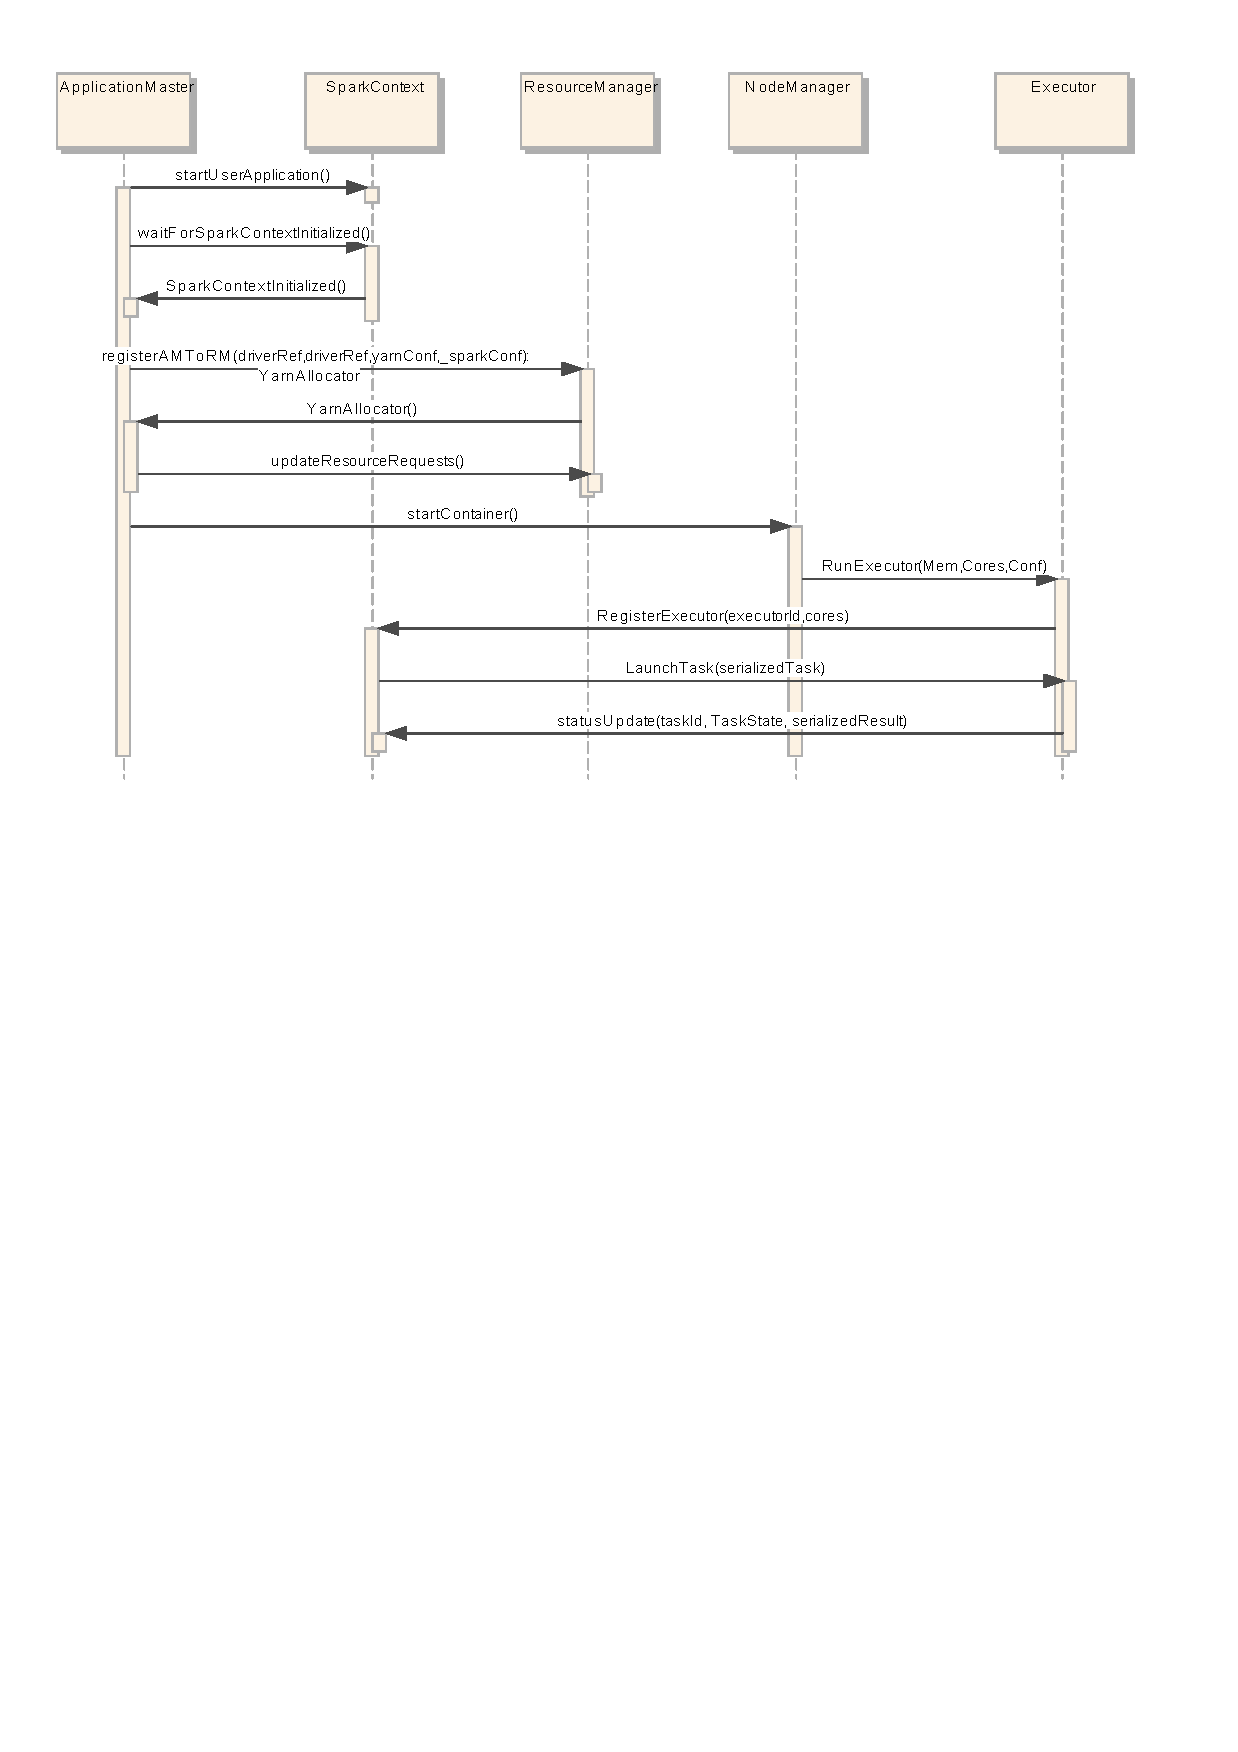
\includegraphics[width=\textwidth]{figures/ExecutorRunTask.pdf}
\caption{Executor运行Task时序图}
\label{fig:ExecutorRunTask}
\end{figure}
\chapter{Spark Shuffle分析}

前面讲解了map端和reduce端对Task的不同处理方式,连接它们的桥梁即为Shuffle模块,shuffle用于打通map任务的输出与reduce任务的输入,map任务计算的中间输出结果按照key值哈希后分配给某一个reduce任务。

shuffle过程数据的传输情况可能非常负责
\begin{enumerate}[\bfseries 1]
	\item 数据量大;
	\item 单个Executor内存不足以放下处理完的数据时需要进行磁盘读写;
	\item 数据传输过程中需要压缩和解压缩;
	\item 跨节点传输时需要通过网络;
\end{enumerate}

正因为这众多的因素,shuffle无疑是调优的重点,理解shuffle的版本历史有助于了解shuffle优化的思路。

Shuffle的类型是在SparkContext初始化时确定的,Spark1.6版本如程序\ref{inputPrg:shuffleManager}所示
\begin{codeInput}{Scala}{ShuffleManager的初始化}{shuffleManager}
 //   指定shuffle的类型
 val shortShuffleMgrNames = Map(
 "hash" -> "org.apache.spark.shuffle.hash.HashShuffleManager",
 "sort" -> "org.apache.spark.shuffle.sort.SortShuffleManager",
 "tungsten-sort" -> "org.apache.spark.shuffle.sort.SortShuffleManager")
 val shuffleMgrName = conf.get("spark.shuffle.manager", "sort")
 val shuffleMgrClass = shortShuffleMgrNames.getOrElse(shuffleMgrName.toLowerCase, shuffleMgrName)
 val shuffleManager = instantiateClass[ShuffleManager](shuffleMgrClass)
\end{codeInput}

可以看出ShuffleManager默认类型为SortShuffleManager。

在Executor上执行ShuffleMapTask时,最终会调用ShuffleMapTask.runTask。核心逻辑如程序\ref{inputPrg:runTaskGetShuffleManager}所示
\begin{codeInput}{Scala}{ShuffleMapTask获取ShuffleWriter}{runTaskGetShuffleManager}
 //从SparkEnv中获取shuffleManager
 val manager = SparkEnv.get.shuffleManager
 //从manager中获取Writer,这里是SortShuffleWriter
 writer = manager.getWriter[Any, Any](dep.shuffleHandle, partitionId, context)
 //调用RDD开始运算,运算结果通过Writer进行持久化,之后将文件所有记录写入并创建索引文件,通过MapStatus告知下游Task
 writer.write(rdd.iterator(partition, context).asInstanceOf[Iterator[_ <: Product2[Any, Any]]])
 writer.stop(success = true).get
\end{codeInput}
\section{Shuffle Writer历史版本}
\subsection{Hash Based Shuffle Write}
在Spark1.0以前,由于不要求数据有序,shuffle write 的任务很简单:将数据 partition 好,并持久化。之所以要持久化,一方面是要减少内存存储空间压力,另一方面也是为了 fault-tolerance。

shuffle write 的任务很简单,那么实现也很简单:将 shuffle write 的处理逻辑加入到 ShuffleMapStage(ShuffleMapTask 所在的 stage) 的最后,该 stage 的 final RDD 每输出一个 record 就将其 partition 并持久化。此种类型的Writer工作方式如图\ref{fig:hashShuffleWriter}所示, 从图中可以看出4 个 ShuffleMapTask 要在同一个 worker node 上运行,CPU core 数为 2,可以同时运行两个 task。每个 task 的执行结果(该 stage 的 finalRDD 中某个 partition 包含的 records)被逐一写到本地磁盘上。每个 task 包含 R 个缓冲区,R = reducer 个数(也就是下一个 stage 中 task 的个数),缓冲区被称为 bucket\footnote{其实 bucket 是一个广义的概念,代表 ShuffleMapTask 输出结果经过 partition后要存放的地方,这里为了细化数据存放位置和数据名称,仅仅用 bucket 表示缓冲区。},其大小为spark.shuffle.file.buffer.kb ,默认是 32KB(Spark 1.1 版本以前是 100KB)。
\begin{figure}[H] 
	\centering
	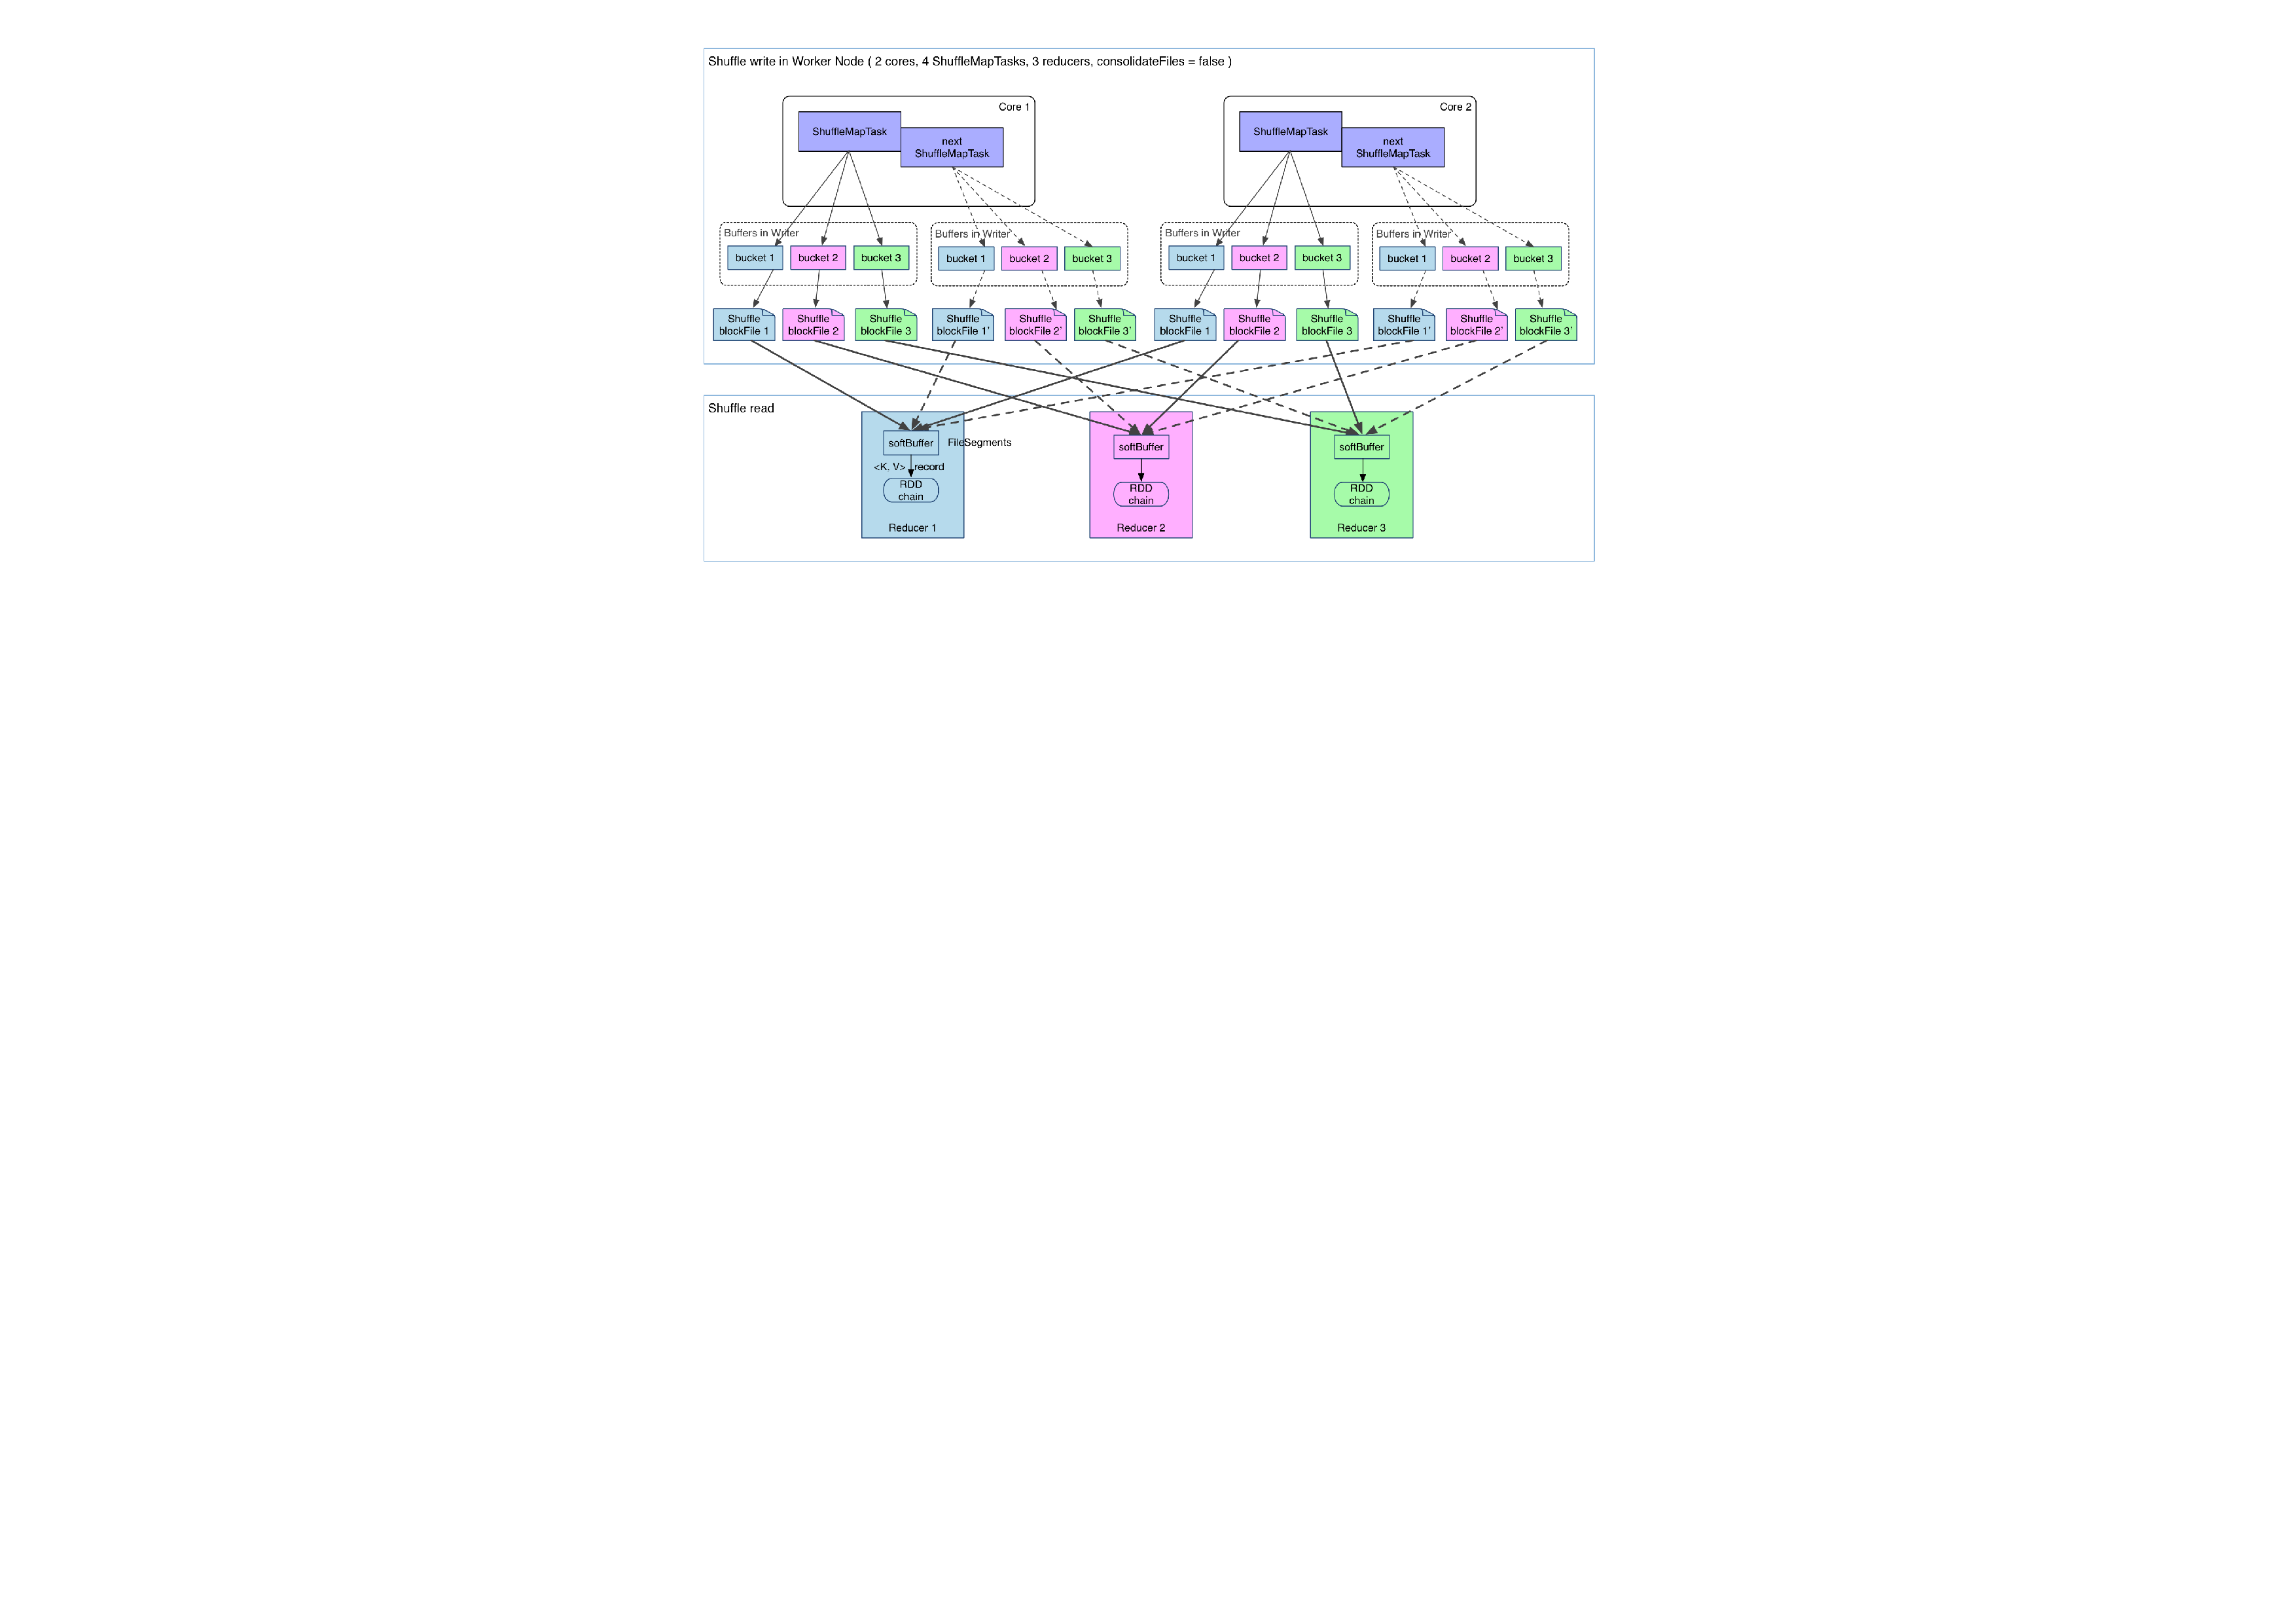
\includegraphics[width=\textwidth]{figures/hashShuffleWriter.pdf}
	\caption{早期的ShuffleWriter工作原理}
	\label{fig:hashShuffleWriter}
\end{figure}
\subsection{Hash Based Shuffle Write存在的问题}

由于ShuffleMapTask需要为每个下游的Task创建一个单独的文件,因此文件的数量就是M*R\footnote{M为shuffleMapTask的数量,R为reduce端Task的数量}个。如果单机28个cpu core,假设节点上20个core用于ShuffleMapTask,R数量为1000个,那么逻辑上会有20000个文件。在实际运行中,Task的数量会更多,这种ShuffleWriter的实现会带来一下问题:
\begin{enumerate}[\bfseries 1]
	\item 缓冲区占用内存空间大
	
	每个节点都可能同时打开多个文件,每次打开文件都会占用一定内存。如上面的20000个文件,每个writer Handler默认需要100KB内存,单个节点就可能达到2GB的内存,当Map端和Reduce同时增加10倍时,整体的内存会更吓人。
	\item 系统随机读增多
	
	当系统存在很多文件比较小但数量比较多的时候,而且机械硬盘在随机读方面的性能特别差,非常容易出现性能瓶颈。
\end{enumerate}
\subsection{Shuffle Consolidate Writer}

为了解决上一小节中Shuffle产生文件较多的问题,之后的Shuffle加入了Consolidate Files机制,它的目标就是减少Shuffle过程文件产生过多的问题,当然第一个问题还是没有解决。它的思想是针对同一个核运行多个ShuffleMapTask的情况下,众多的ShuffleMapTask会将记录写到同一个文件中,下一个会以追加的方式写入而不是新建文件。这样文件数就变为core\footnote{这里指核的数量}*R个文件。此种模式下运行原理如图\ref{fig:consolidate}所示
\begin{figure}[H] 
	\centering
	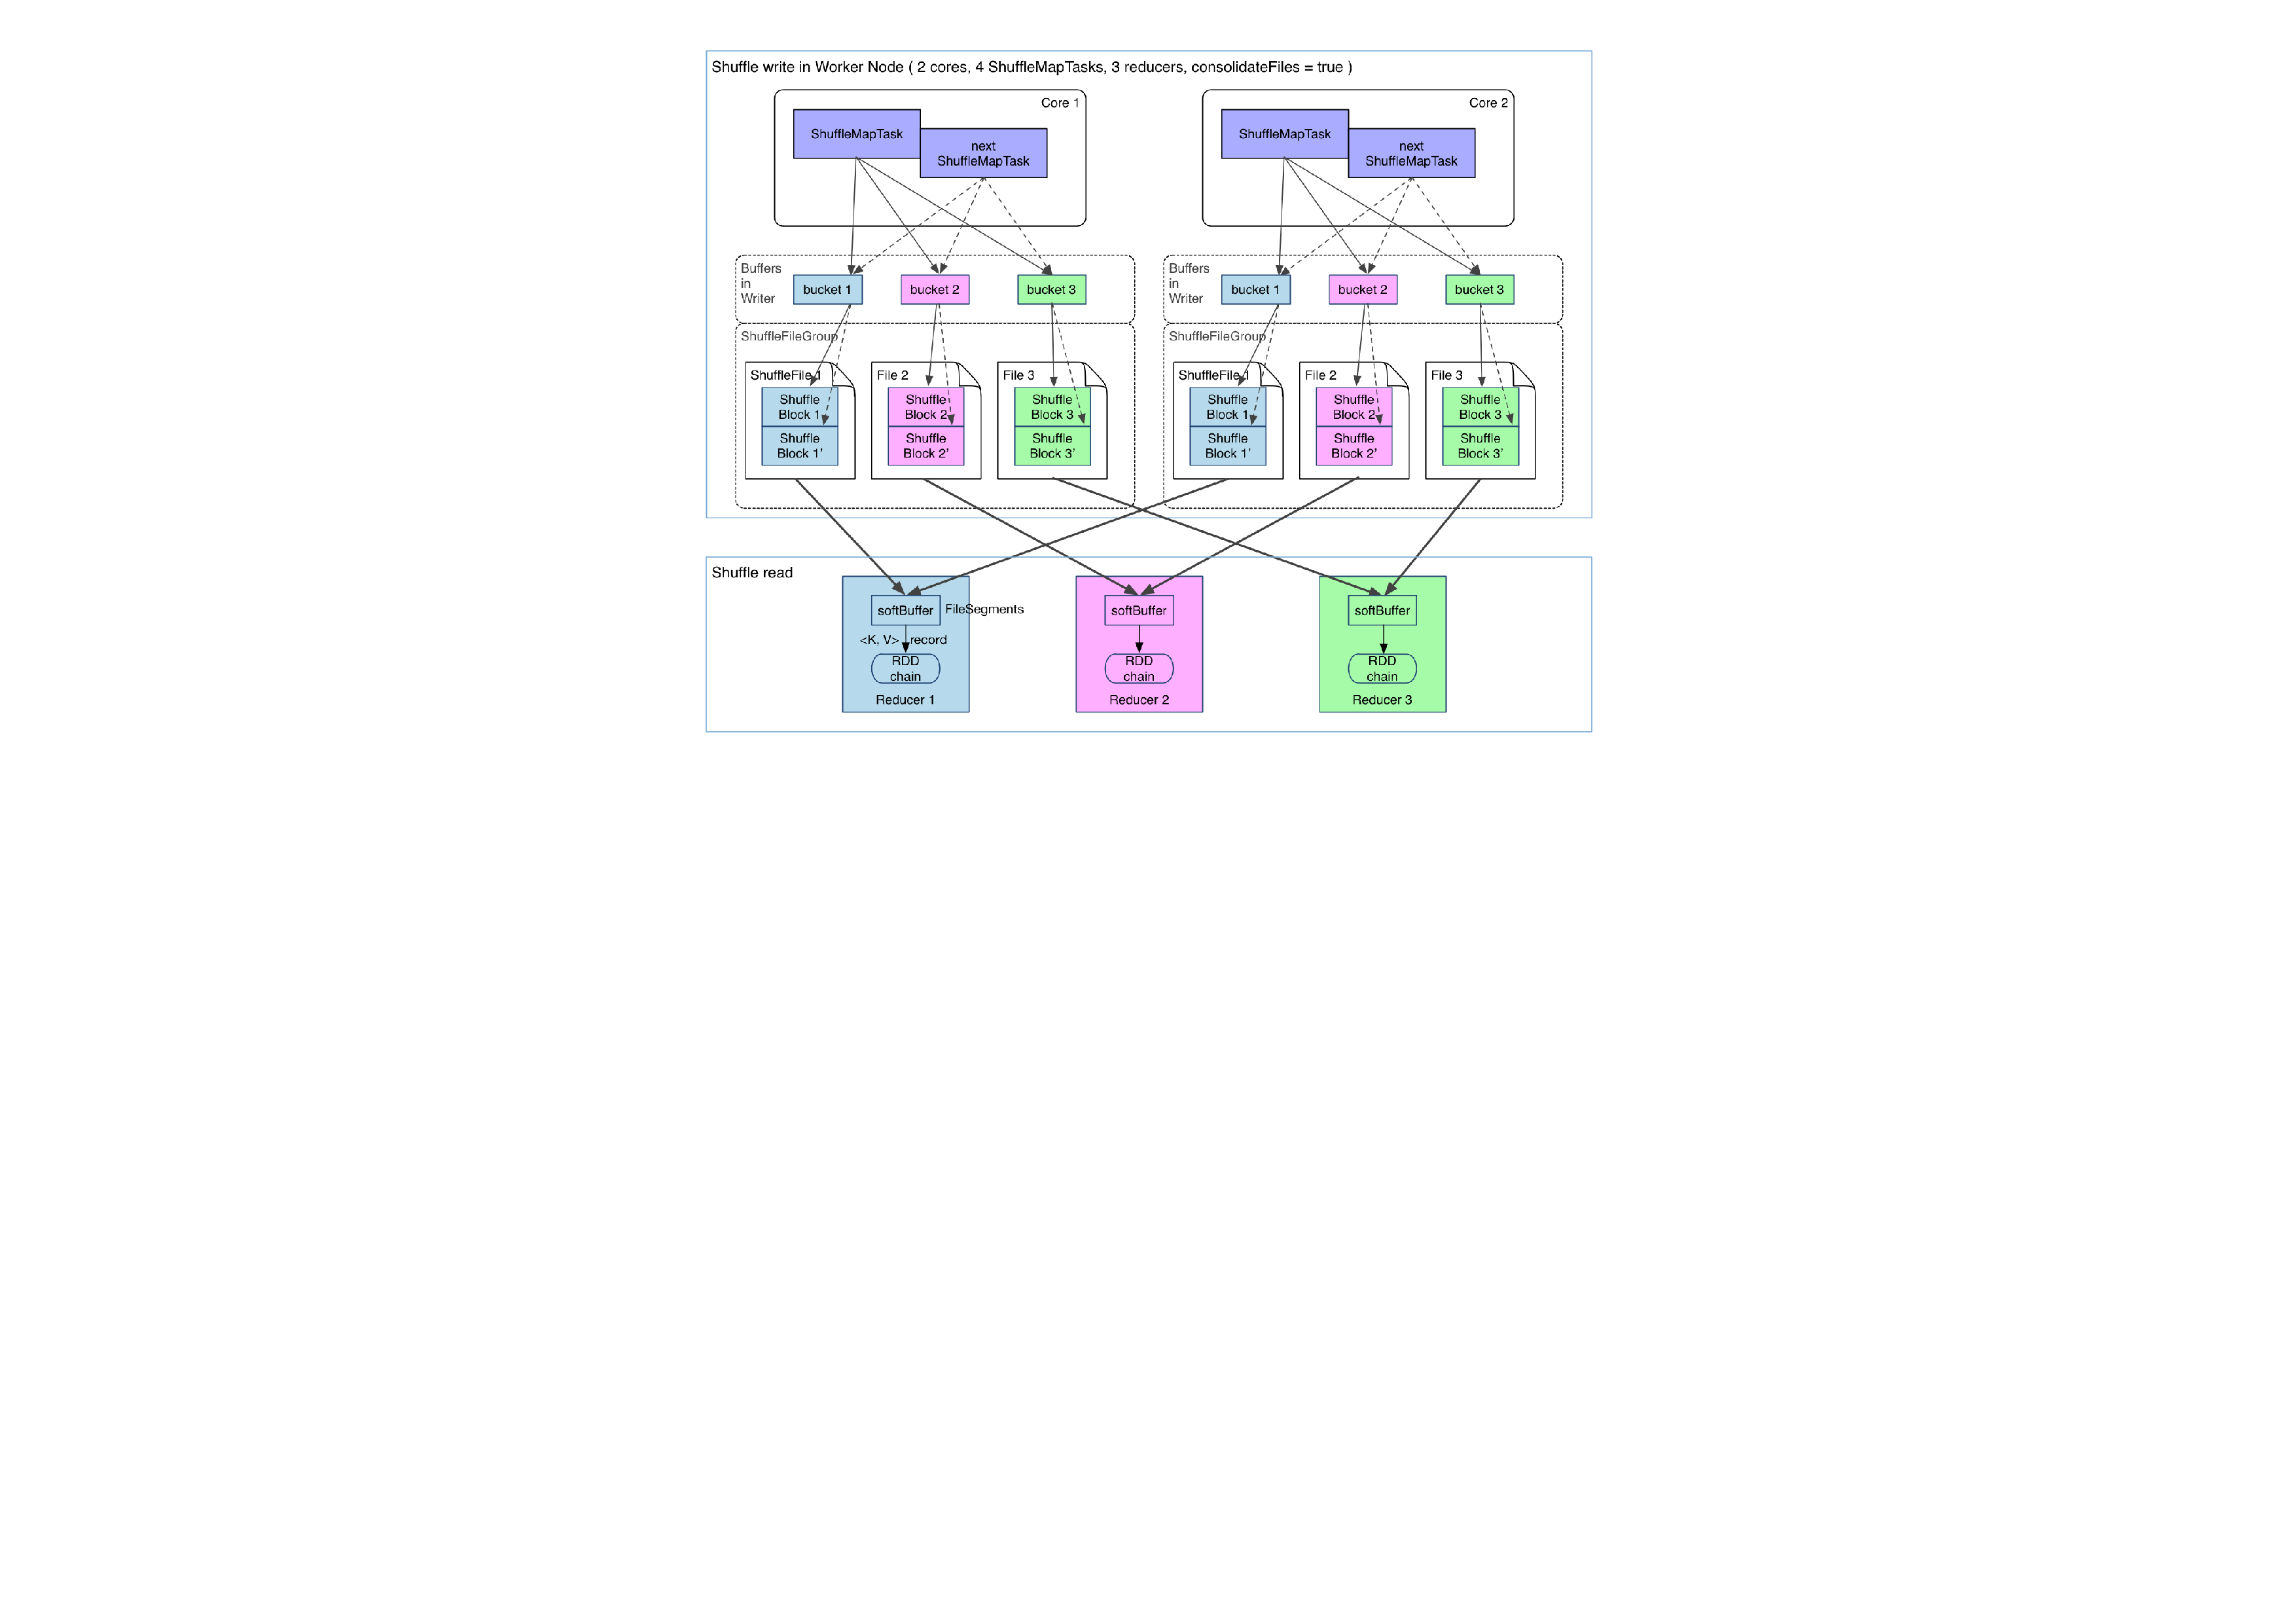
\includegraphics[width=\textwidth]{figures/consolidate.pdf}
	\caption{Shuffle Consolidate Files工作原理}
	\label{fig:consolidate}
\end{figure}

不过这种模式下当每个core只运行一个ShuffleMapTask时,那么就和原来的机制一样了。但是当ShuffleMapTask明显多于core数量时,这种模式下可以显著减少文件的数量。这里还剩下一个问题,下游的Task如何区分文件的不同部分?这部分在后面小节中讲述。

针对Shuffle Consolidate遗留的问题,Spark重新建立了一套Shuffle机制。也就是下面讲述的SortShuffle,这个已经是当前Spark版本的默认选项。
\subsection{Sort Based Write}
此方法的选择是在org.apache.spark.SparkEnv下完成的,本章开头部分已经说明。首先,每个ShuffleMapTask不会为每个Reducer生成一个单独的文件相反,它会将所有的结果写到一个文件里,同时生成一个Index文件,Reducer可以通过这个Index文件取得它需要处理的数据,减少了文件的数量。

Shuffle Map Task 会按照 key 相对应的 partition id 进行排序,对于属于同一个 partition 的 keys 可选的进行或不进行排序。因为对于不需要排序的操作来说,这个排序是有损性能的。对于那些需要 Sort 的操作,比如 sortByKey,这个排序是由 Reducer 完成的。Sort Base Shuffle原理如图\ref{fig:sortshuffle}所示
\begin{figure}[H] 
	\centering
	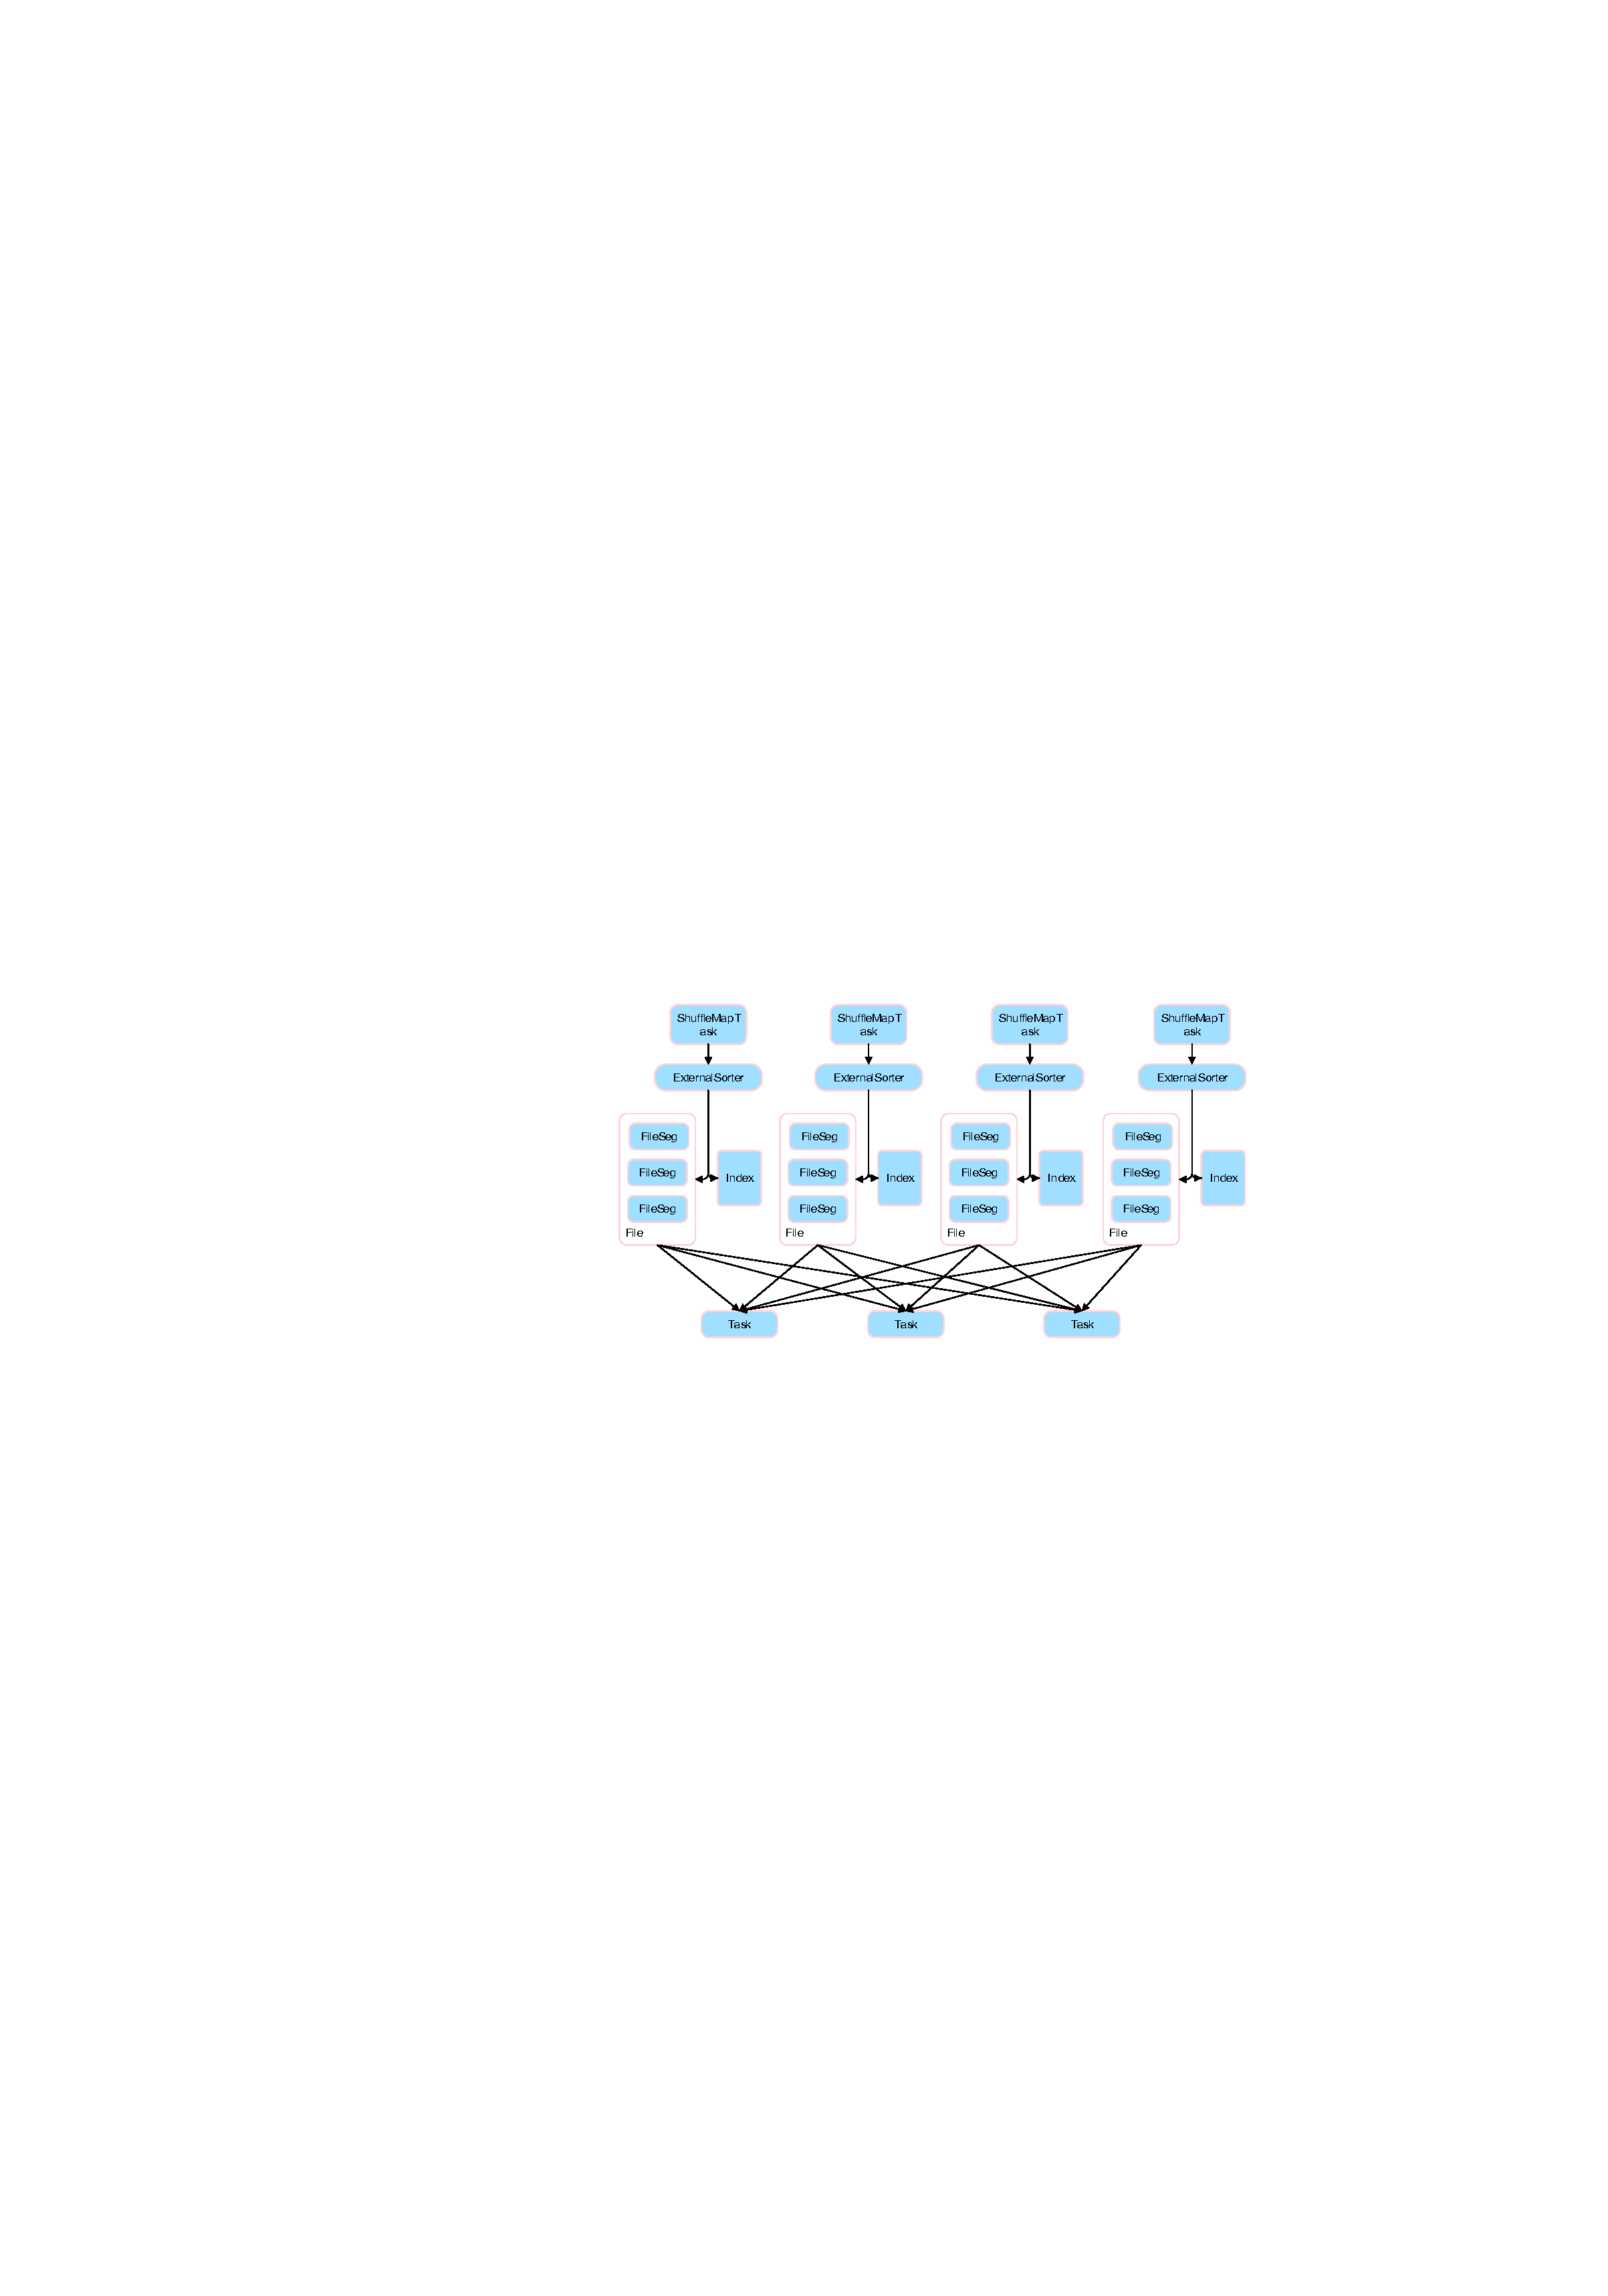
\includegraphics[width=\textwidth]{figures/sortshuffle.pdf}
	\caption{Sort Base Shuffle工作原理}
	\label{fig:sortshuffle}
\end{figure}

为了下游Task获取到其所需要的分区,生成文件的同时会附加Index文件,来记录不同分区的位置信息。
\section{Spark1.6版本Shuffle Write}
本节分析Spakr1.6中默认采用的SortShuffleManager对应的writer。SortShuffleManager中的getWriter会根据不同的ShuffleHandle产生相应的ShuffleWriter
\begin{enumerate}[\bfseries 1]
	\item SerializedShuffleHandle 对应 UnsafeShuffleWriter
	\item BypassMergeSortShuffleHandle 对应 BypassMergeSortShuffleWriter
	\item BaseShuffleHandle 对应 SortShuffleWriter
\end{enumerate}
\subsection{BaseShuffleHandle 对应 SortShuffleWriter}
其writer方法如程序\ref{inputPrg:sortShuffleWriter}所示
\begin{codeInput}{Scala}{SortShuffleWriter write方法实现}{sortShuffleWriter}
override def write(records: Iterator[Product2[K, V]]): Unit = {
  //如果数据需要在map端combine,则需要传入dep.aggregator,下面的这个dep.keyOrdering是空值,
  // 因为在spark的sortedshuffle中,数据是不排序的。这里的这个partitioner是用来为后续RDD构造partitions的
  sorter = if (dep.mapSideCombine) {
    require(dep.aggregator.isDefined, "Map-side combine without Aggregator specified!")
    new ExternalSorter[K, V, C](
    context, dep.aggregator, Some(dep.partitioner), dep.keyOrdering, dep.serializer)
  } else {
    //如果数据不需要在map端combine,则aggregator传None就行
    new ExternalSorter[K, V, V](context, aggregator = None, Some(dep.partitioner), ordering = None,dep.serializer)
  }
  //将数据先放入缓存中,如果缓存不够用spill到磁盘,在这一步也会对相同key值的数据进行combine操作
  sorter.insertAll(records)
  //打开一个文件
  val output = shuffleBlockResolver.getDataFile(dep.shuffleId, mapId)
  val tmp = Utils.tempFileWith(output)
  //构造blockId
  val blockId = ShuffleBlockId(dep.shuffleId, mapId, IndexShuffleBlockResolver.NOOP_REDUCE_ID)
  //将数据写入data文件
  val partitionLengths = sorter.writePartitionedFile(blockId, tmp)
  //将数据写入index文件
  shuffleBlockResolver.writeIndexFileAndCommit(dep.shuffleId, mapId, partitionLengths, tmp)
  //进行shuffle read时的一些参考信息
  mapStatus = MapStatus(blockManager.shuffleServerId, partitionLengths)
}
\end{codeInput}
程序\ref{inputPrg:sortShuffleWriter}中的ExternalSorter有下面三个作用
\begin{enumerate}
	\item 实例化ExternalSorter
	\item 调用insertAll()方法对记录集进行操作
	\item 返回已经排序或者聚合之后的记录的迭代器
\end{enumerate}
\subsection{实例化ExternalSorter}
首先就是实例化ExternalSorter,这里有一个判断,如果要进行map端的combine操作的话就需要指定Aggregator和Ordering,否则这两个参数为None。本例采用的reduceByKey就进行了Map端的combine操作,由ReduceByKey算子构造ShuffleRDD的过程如图\ref{fig:instantiateExternalSorter}所示
\begin{figure}[H] 
	\centering
	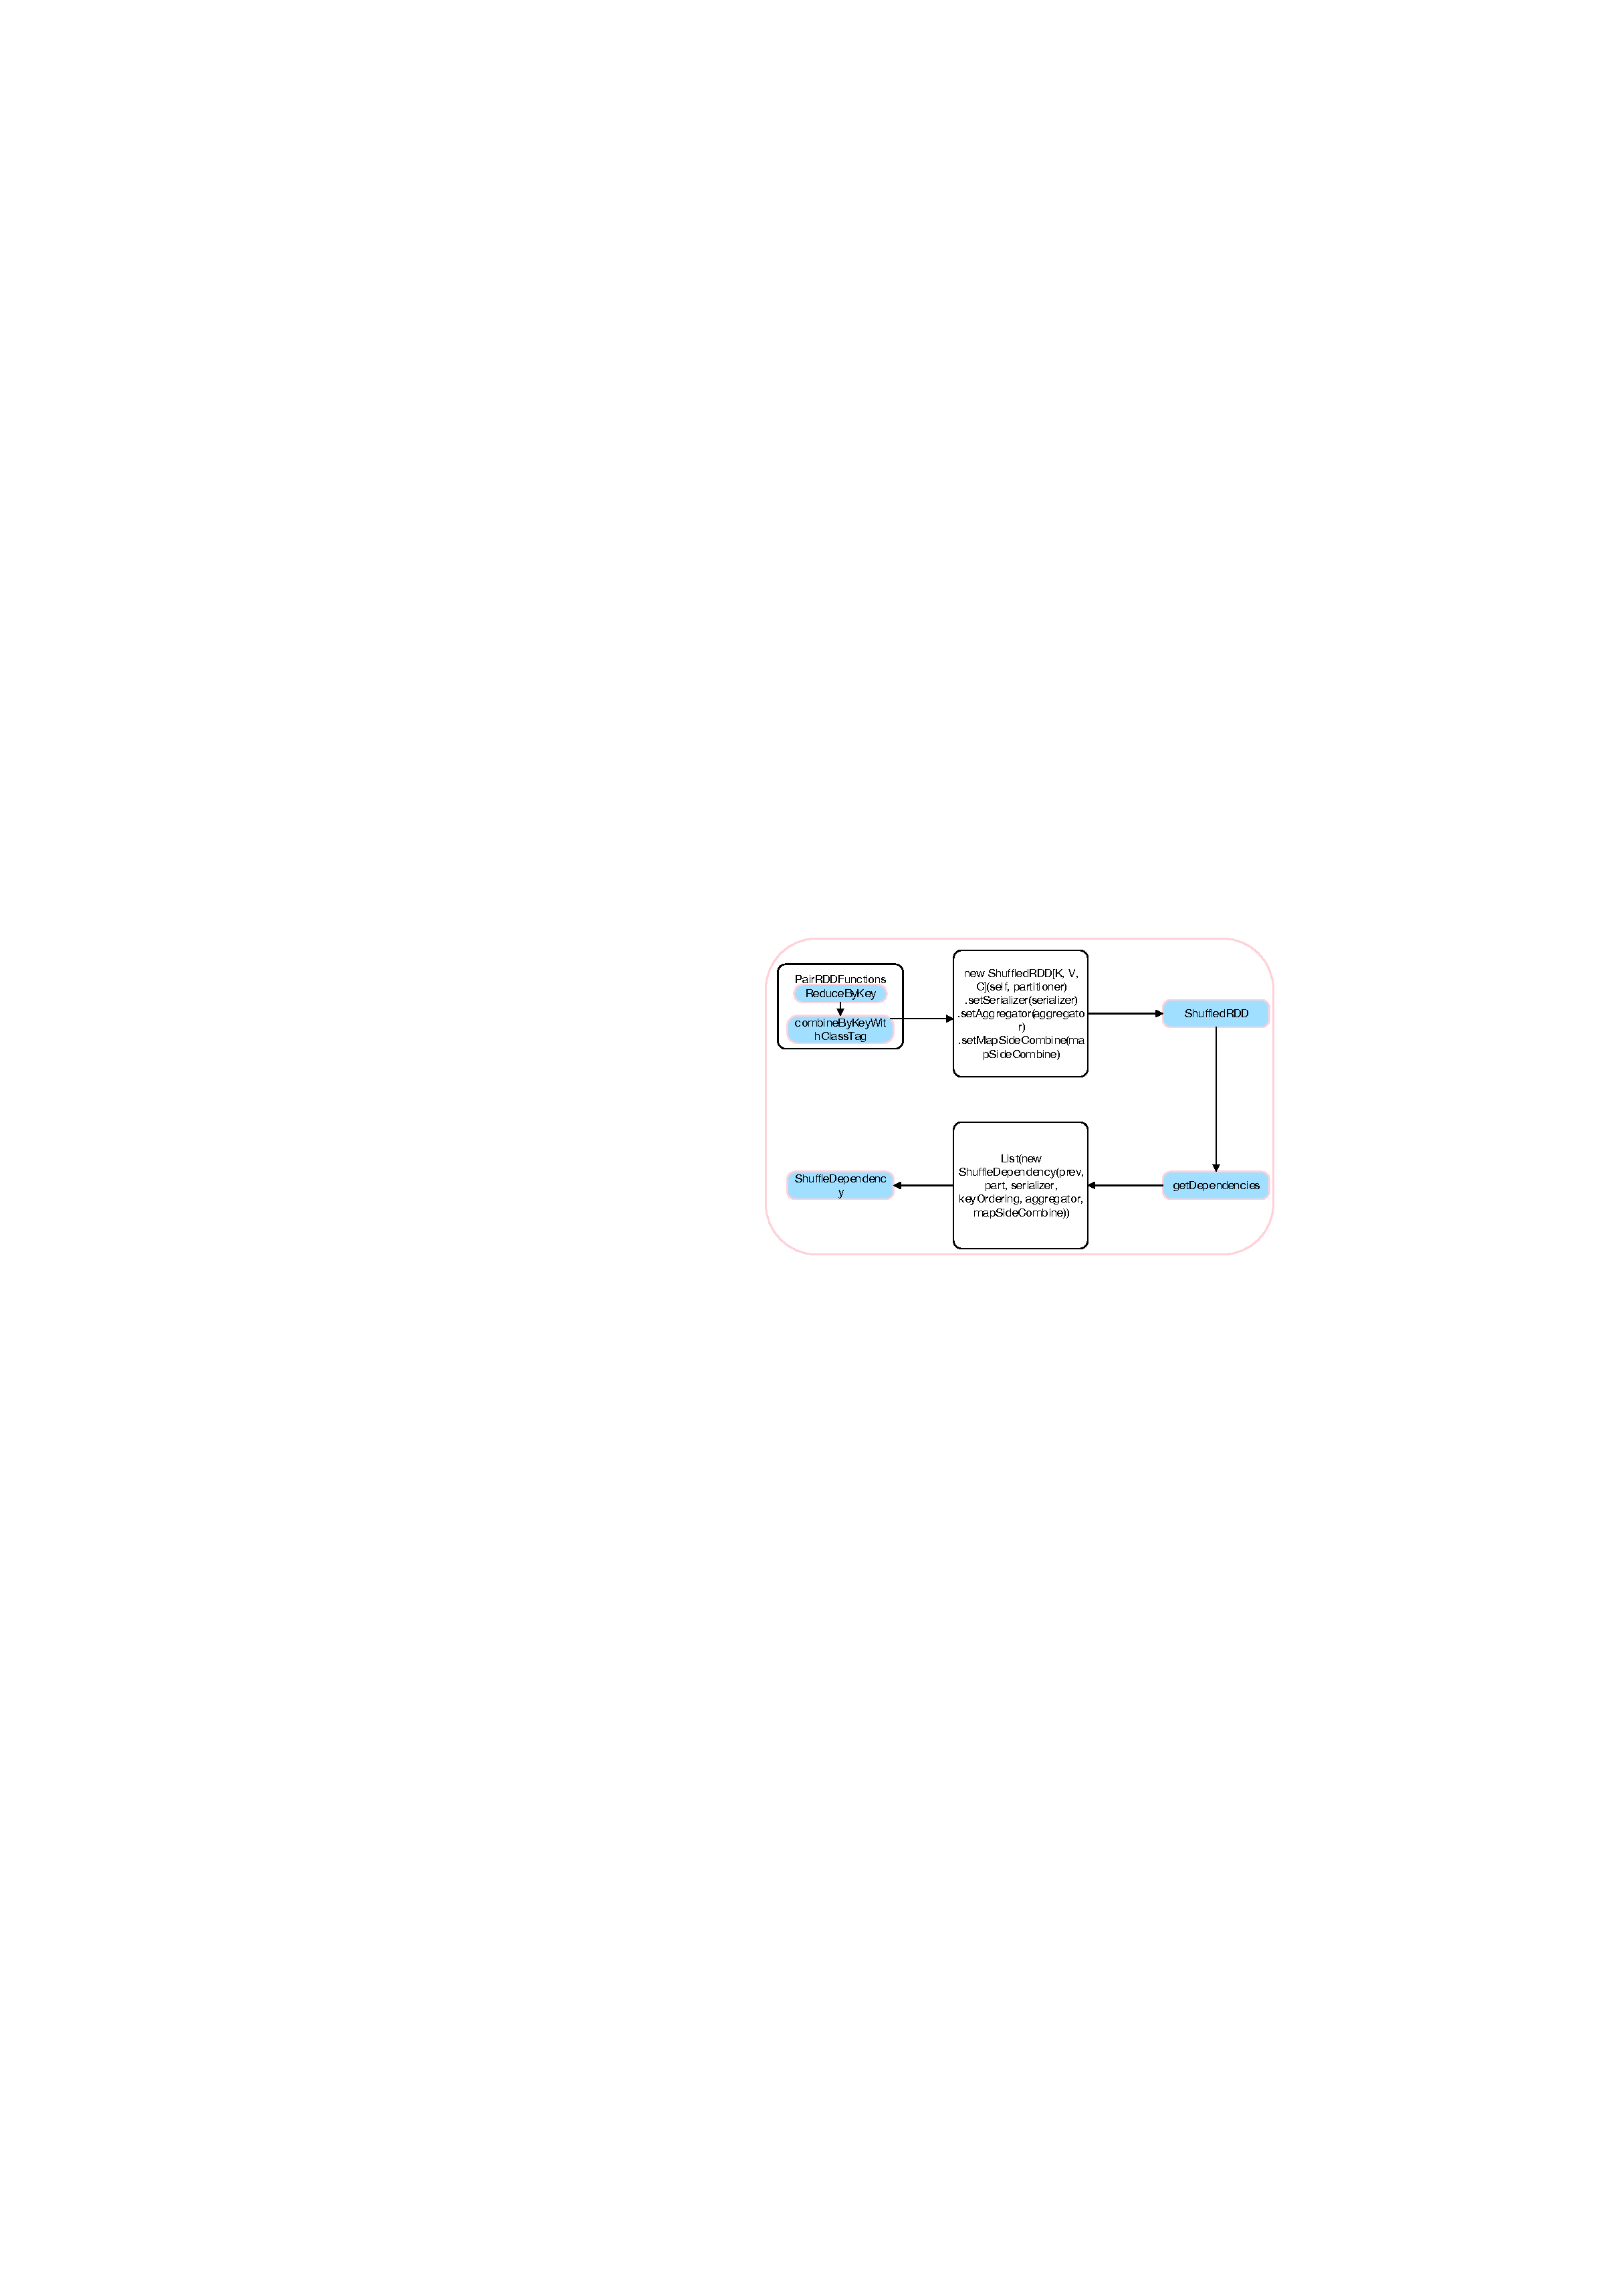
\includegraphics[width=\textwidth]{figures/ReduceByKey.pdf}
	\caption{ReduceByKey算子}
	\label{fig:instantiateExternalSorter}
\end{figure}
\subsection{shuffle写操作}
通过判断是否进行Map端combine操作而实例化出不同的ExternalSorter后,就会调用insertAll方法,将输入的记录写入到内存中,如果内存不足就spill到磁盘中,具体的实现我们来看insertAll方法,如程序\ref{inputPrg:insertAll}所示
\begin{codeInput}{Scala}{SortShuffleWriter insertAll方法实现}{insertAll}
def insertAll(records: Iterator[Product2[K, V]]): Unit = {
  val shouldCombine = aggregator.isDefined	
  //首先判断是否需要进行Map端的combine操作
  if (shouldCombine) {
    //如果需要进行Map端combine操作,使用PartitionedAppendOnlyMap作为缓存
    // mergeValue其实就是我们用reduceByKey的时候参数值,即_+_
    val mergeValue = aggregator.get.mergeValue
    //(C, V) => C  =>func
    //createCombiner其实是和mergeValue一样的,都是_+_,但是在使用createCombiner中只传了一个参数,所以另一个参///数默认采用默认值,这里为0
    val createCombiner = aggregator.get.createCombiner//V => C
    var kv: Product2[K, V] = null
    // 这个update也是一个函数,逻辑为如果某个Key已经存在记录record就使用上面获取的聚合函数进行聚合操作,
    // 如果不存在记录,就使用createCombiner方法进行初始化操作
    val update = (hadValue: Boolean, oldValue: C) => {
      if (hadValue) mergeValue(oldValue, kv._2) else createCombiner(kv._2)
    }
    //遍历所有的records
    while (records.hasNext) {
      //记录spill的频率,每当read一条record的时候就会记录一次
      addElementsRead()
      //使用kv存储当前读的records
      kv = records.next()
      //对key相同的记录的value进行合并
      //更新map中的数据,其中private var map = new PartitionedAppendOnlyMap[K, C],
      // 如果需要进行combine就将数据放在map中,然后在map中对数据进行更新操作
      map.changeValue((getPartition(kv._1), kv._1), update)
      //判断是否需要进行spill操作
      maybeSpillCollection(usingMap = true)
    }
  } else {
    // 如果不需要进行Map端的聚合操作,就直接将记录放到buffer(PartitionedPairBuffer)中
    while (records.hasNext) {
      addElementsRead()
      val kv = records.next()
      buffer.insert(getPartition(kv._1), kv._1, kv._2.asInstanceOf[C])
      maybeSpillCollection(usingMap = false)
    }
  }
}
\end{codeInput}
PartitionedAppendOnlyMap和PartitionedPairBuffer其类图如图\ref{fig:mapAndBuffer}所示
\begin{figure}[H] 
	\centering
	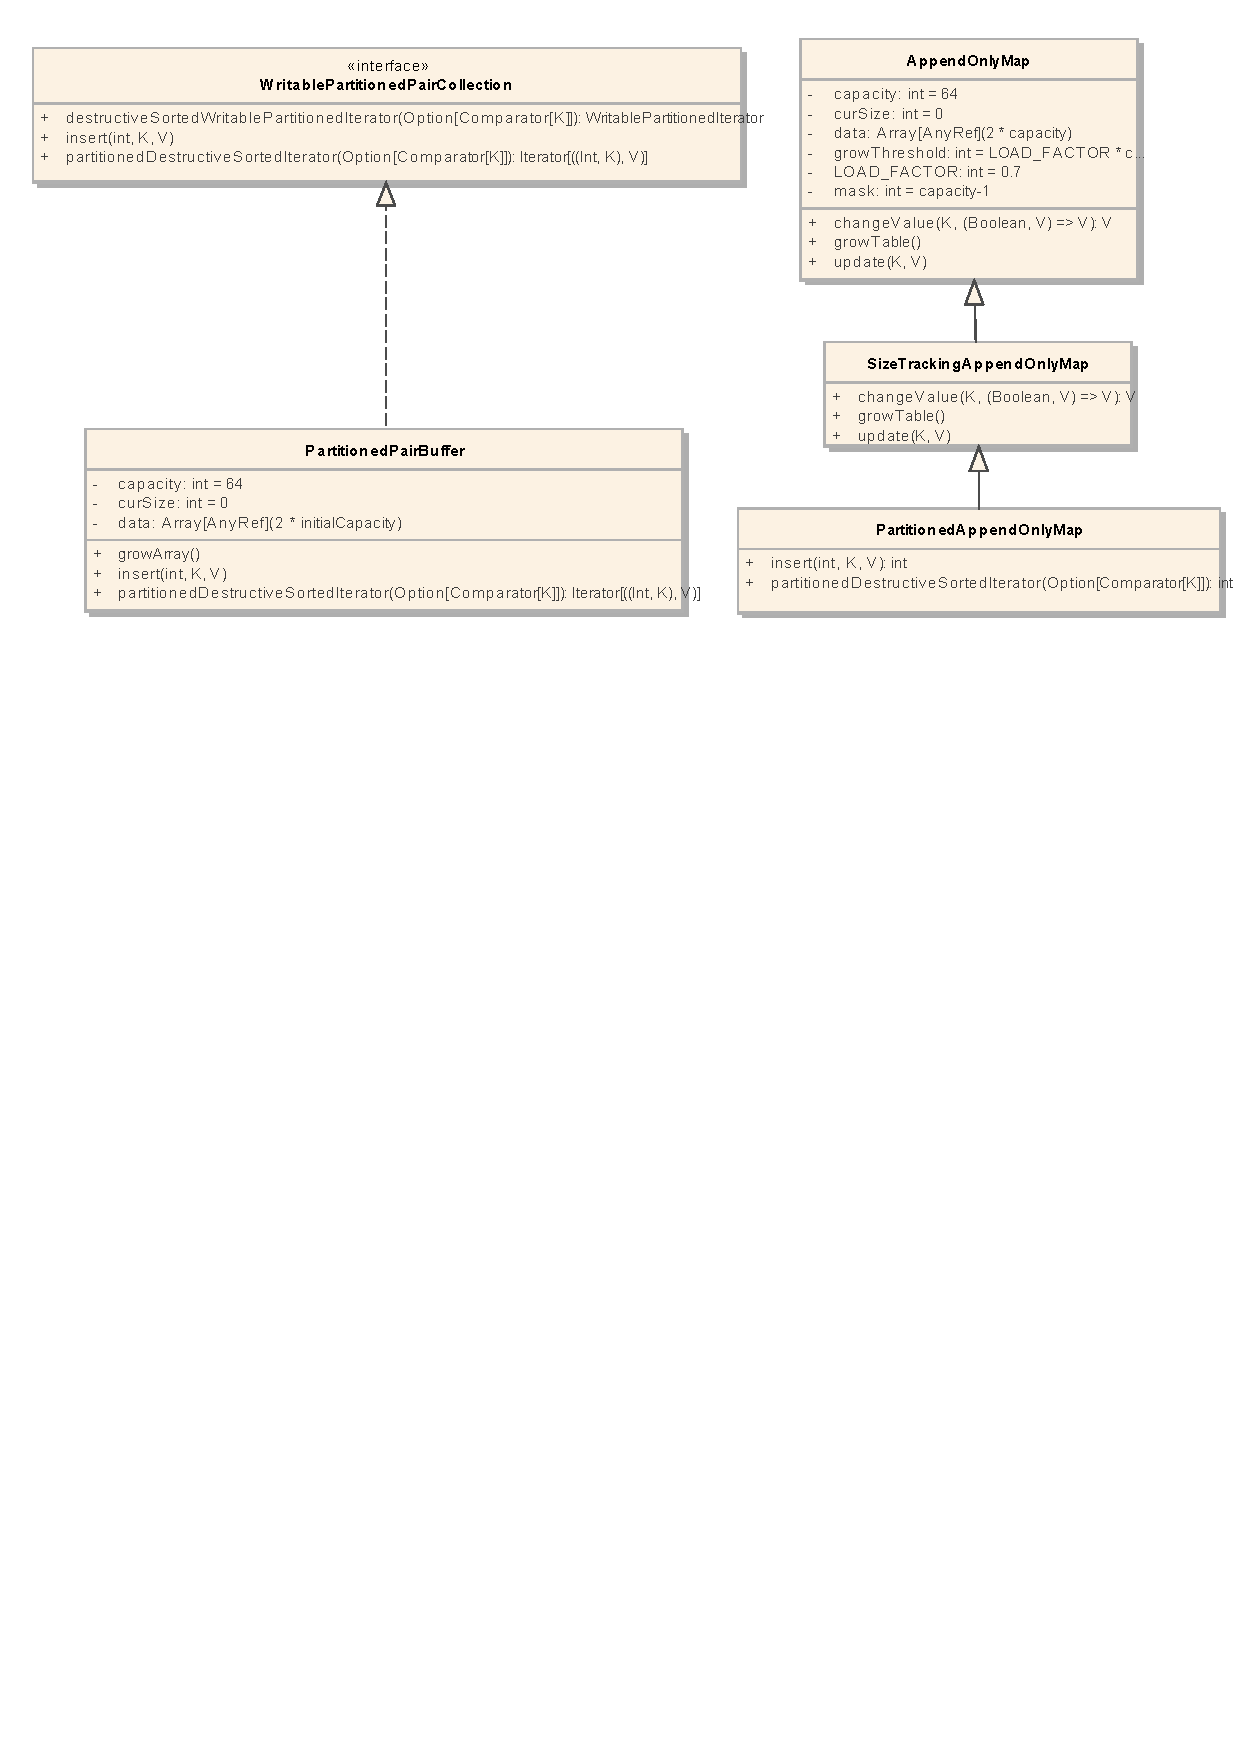
\includegraphics[width=\textwidth]{figures/collection.pdf}
	\caption{Map和Buffer类图}
	\label{fig:mapAndBuffer}
\end{figure}

由上图可以看出reduceBy算法需要map端聚合,map.changeValue调用的是AppendOnlyMap中的changeValue,完成的工作是将记录写到map缓存中,按照reduceByKey算子中定义的合并方法对相同key的value进行处理。如程序\ref{inputPrg:mapChangeValue}所示
\begin{codeInput}{Scala}{缓存并更新value值}{mapChangeValue}
def changeValue(key: K, updateFunc: (Boolean, V) => V): V = {
  assert(!destroyed, destructionMessage)
  val k = key.asInstanceOf[AnyRef]
  //如果传入的key为空值,队列自动增加长度,
  // 这里的设计很巧妙:因为队列自动增加,就肯定会多出一个值,如果你不给它赋值的话,它就为null,
  // 但是这个值又不占队列中具体的位置,只要在最后的时候保留一个没有赋值的位置即可。
  if (k.eq(null)) {
    if (!haveNullValue) {
      incrementSize()
    }
    nullValue = updateFunc(haveNullValue, nullValue)
    haveNullValue = true
    return nullValue
  }
  var pos = rehash(k.hashCode) & mask
  var i = 1
  while (true) {
    //data是一个数组,用来同时存储key和value:key0, value0, key1, value1, key2, value2, etc.
    // 即2 * pos上存储的是key的值,2 * pos + 1上存储的是value的值
    val curKey = data(2 * pos)
    if (k.eq(curKey) || k.equals(curKey)) {
      //如果有相同的值的话,则根据updateFunc更新这个key对应的value
      val newValue = updateFunc(true, data(2 * pos + 1).asInstanceOf[V])
      data(2 * pos + 1) = newValue.asInstanceOf[AnyRef]
      return newValue
    } else if (curKey.eq(null)) {
      //如果key不存在就将该key和对应的value添加到data这个数组中
      val newValue = updateFunc(false, null.asInstanceOf[V])
      data(2 * pos) = k
      data(2 * pos + 1) = newValue.asInstanceOf[AnyRef]
      incrementSize()
      return newValue
    } else {
      //如果pos和其它的key重合,则继续计算其位置
      val delta = i
      pos = (pos + delta) & mask
      i += 1
    }
  }
  null.asInstanceOf[V] // Never reached but needed to keep compiler happy
}
\end{codeInput}
\subsection{shuffle结果本地缓存}
这部分将shuffle结果缓存到本地,并为之生成索引文件,同时返回文件的迭代器。整体过程如程序\ref{inputPrg:cachePartitionFile}所示
\begin{codeInput}{Scala}{完成分区文件和索引文件的本地缓存}{cachePartitionFile}
//打开一个文件
val output = shuffleBlockResolver.getDataFile(dep.shuffleId, mapId)
val tmp = Utils.tempFileWith(output)
//构造blockId
val blockId = ShuffleBlockId(dep.shuffleId, mapId, IndexShuffleBlockResolver.NOOP_REDUCE_ID)
//将数据写入data文件
val partitionLengths = sorter.writePartitionedFile(blockId, tmp)
//将数据写入index文件
shuffleBlockResolver.writeIndexFileAndCommit(dep.shuffleId, mapId, partitionLengths, tmp)
//进行shuffle read时的一些参考信息
mapStatus = MapStatus(blockManager.shuffleServerId, partitionLengths)
\end{codeInput}
\subsubsection{写分区文件}
此步骤负责将缓存在内存map或者buffer中的记录缓存到本地磁盘中,如果之前已经有部分数据溢出到磁盘,会将这些一起进行合并。写分区文件过程如程序\ref{inputPrg:writePartitionFile}所示
\begin{codeInput}{Scala}{生成分区文件并写入数据}{writePartitionFile}
def writePartitionedFile(
blockId: BlockId,
outputFile: File): Array[Long] = {
  val lengths = new Array[Long](numPartitions)
  //首先判断是否有数据已经spill到磁盘了
  if (spills.isEmpty) {
    //当只有内存中有数据时
    val collection = if (aggregator.isDefined) map else buffer
    // 获得迭代器
    val it = collection.destructiveSortedWritablePartitionedIterator(comparator)
    //进行迭代并将数据写到磁盘
    while (it.hasNext) {
      val writer = blockManager.getDiskWriter(blockId, outputFile, serInstance, fileBufferSize,context.taskMetrics.shuffleWriteMetrics.get)
      val partitionId = it.nextPartition()
      while (it.hasNext && it.nextPartition() == partitionId) {
        //把同一个分区的记录写到一块 并返回该blockId中该partitionId的长度
        it.writeNext(writer)
      }
      writer.commitAndClose()
      val segment = writer.fileSegment()
      //最后返回的是每个partition写入数据的长度
      lengths(partitionId) = segment.length
    }
  } else {
    //需要持久化到硬盘中的情况,在调用partitionedIterator方法后,会对应的partition中的已经combine过的数据
    for ((id, elements) <- this.partitionedIterator) {
      if (elements.hasNext) {
        val writer = blockManager.getDiskWriter(blockId, outputFile, serInstance, fileBufferSize,
        context.taskMetrics.shuffleWriteMetrics.get)
        //将partition中的数据写入data文件
        for (elem <- elements) {
          writer.write(elem._1, elem._2)
        }
        writer.commitAndClose()
        val segment = writer.fileSegment()
        //最后返回的是每个partition写入数据的长度
        lengths(id) = segment.length
      }
    }
  }
//更改task测量系统中的参数值
......
lengths
}
\end{codeInput}

上面函数通过判断spills是否为空进行了不同的处理,spills为空时表示记录全部缓存在内存中只需要从内存map或者buffer中取出数据写到本地磁盘即可,spills不为空时,得将已经写到磁盘的和内存中缓存的部分进行合并。接下来分析spills为空时的情况。

程序会获取collection的迭代器,这里会传入比较器,其中destructiveSortedWritablePartitionedIterator是个接口方法,其内部逻辑如程序\ref{inputPrg:destructiveSortedWritablePartitionedIterator}所示
\begin{codeInput}{Scala}{排序分区迭代器}{destructiveSortedWritablePartitionedIterator}
def destructiveSortedWritablePartitionedIterator(keyComparator: Option[Comparator[K]])
: WritablePartitionedIterator = {
  // 这里的partitionedDestructiveSortedIterator会根据是map或者buffer有不同的实现
  val it = partitionedDestructiveSortedIterator(keyComparator)
  // 最后返回的是WritablePartitionedIterator,上面进行写操作的时候就是调用该迭代器中的writeNext方法
  new WritablePartitionedIterator {
    private[this] var cur = if (it.hasNext) it.next() else null	
    def writeNext(writer: DiskBlockObjectWriter): Unit = {
      writer.write(cur._1._2, cur._2)//((partitionId,K),V)
      cur = if (it.hasNext) it.next() else null
    }	
    def hasNext(): Boolean = cur != null	
    def nextPartition(): Int = cur._1._1
  }
}
\end{codeInput}

程序\ref{inputPrg:destructiveSortedWritablePartitionedIterator}中partitionedDestructiveSortedIterator会根据是map或者buffer有不同的实现,由图\ref{fig:mapAndBuffer}可以看出map时其实现在PartitionedAppendOnlyMap,从其实现上可以看出排序逻辑,如程序\ref{inputPrg:PartitionedAppendOnlyMapIter}所示
\begin{codeInput}{Scala}{PartitionedAppendOnlyMap分区排序迭代器实现}{PartitionedAppendOnlyMapIter}
def partitionedDestructiveSortedIterator(keyComparator: Option[Comparator[K]])
: Iterator[((Int, K), V)] = {
  //先它这里会构造一个按partition和key进行比较的比较器,这个比较器先按partition来排序,
  //然后再用key的hashcode进行排序,记住这里spark系统是进行key排序了的,而不是没有排序,只是它这里是按照key的hashcode进行的排序。
  val comparator = keyComparator.map(partitionKeyComparator).getOrElse(partitionComparator)
  //后通过这个比较器再对这个map进行排序
  destructiveSortedIterator(comparator)
}
\end{codeInput}
\subsubsection{写索引文件}
具体的实现就不详细说明了,主要就是根据上一步的到的partition长度的数组将偏移量写入到index文件中。

所以最终每一个task的文件最终产生两个文件,而一个spark程序shuffle产生的数据就取决于并行度或者说reducer的数量,即2*recuder个。

最后就是实例化MapStatus,shuffle read的时候根据MapStatus获取数据。

\subsection{BypassMergeSortShuffleHandle对应BypassMergeSortShuffleWriter}
该writer在进行写记录之前会根据reducer的个数(例如R个)生成R个临时文件,然后将记录写入对应的临时文件中,最后将这些文件进行合并操作并写入到一个文件中,由于直接将记录写入了临时文件,并没有缓存在内存中,所以如果reducer的个数过多的话,就会为每个reducer打开一个临时文件,如果reducer的数量过多的话就会影响性能,所以使用该种方式需要满足一些条件
\begin{enumerate}[\bfseries 1]
	\item 无排序器
	\item 无聚合器
	\item reduce端分区数量<spark.shuffle.sort.bypassMergeThreshold.默认值为200
\end{enumerate}

\subsection{SerializedShuffleHandle对应UnsafeShuffleWriter}

这部分也就是通常所说的Tungsten,在此不做细讲。
\subsection{Shuffle Write流程图}
\begin{figure}[H] 
	\centering
	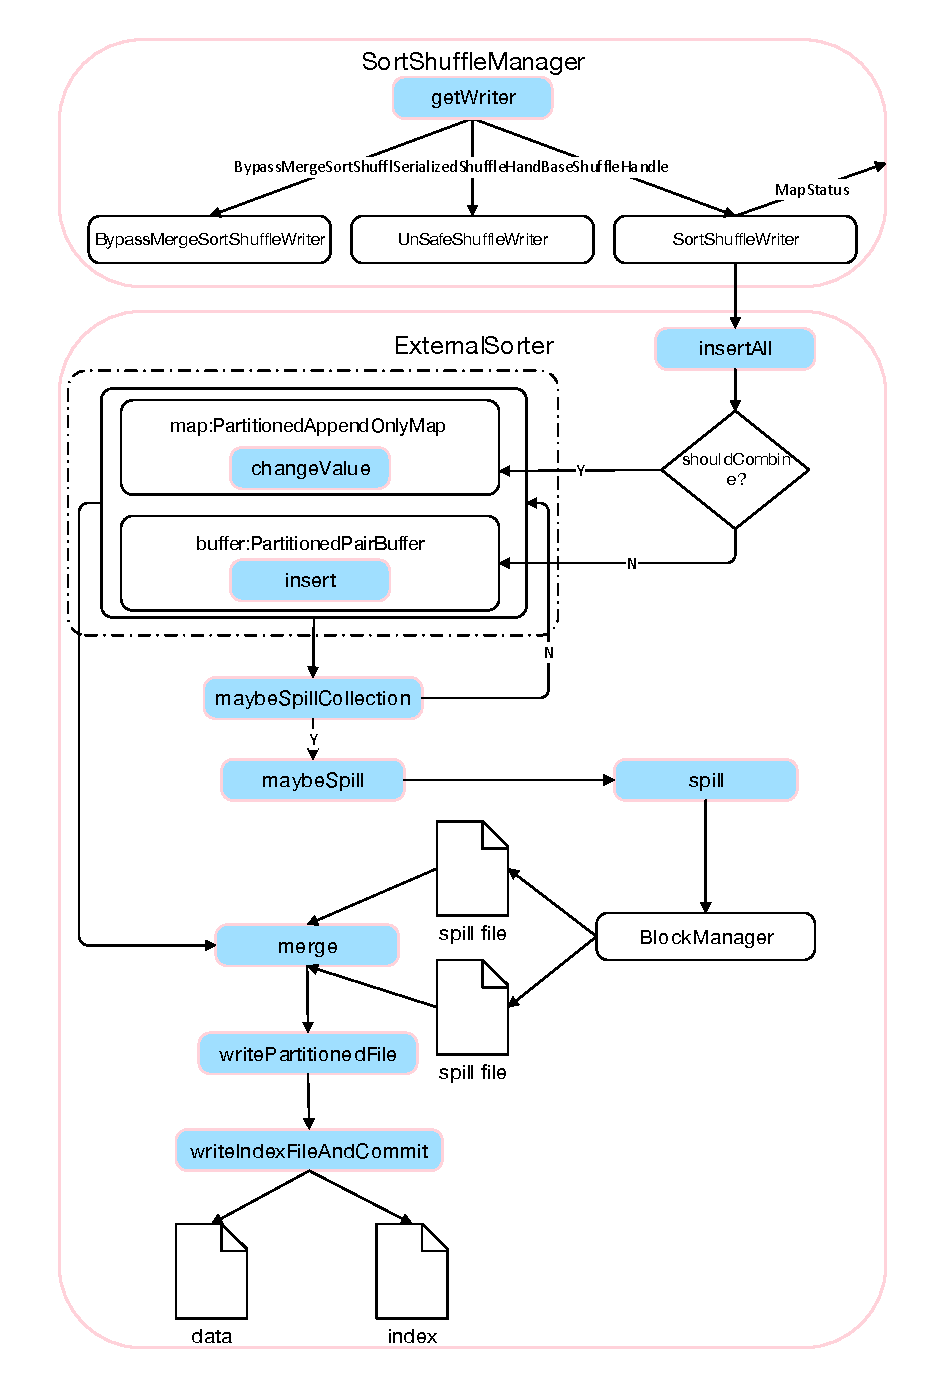
\includegraphics[width=\textwidth,height=0.9\textheight]{figures/sortShuffleWriter.pdf}
	\caption{SortShuffleWriter流程图}
	\label{fig:sortShuffleWriter}
\end{figure}
SortShuffleWriter具体流程如图\ref{fig:sortShuffleWriter}所示
\section{Spark1.6版本Shuffle Read}

在Stage的边界,要计算ShuffledRDD中的数据,必须先把 MapPartitionsRDD 中的数据 fetch 过来。而下边界,要么将文件写入本地文件系统,以供子Stage读取,要么是最后一个Stage,输出结果。

下游Stage的第一个RDD即为ShuffledRDD,其compute方法中会调用shuffleManager.getReader来读取上游的分区,而不管是HashShuffleManager还是SortShuffleManager,其getReader方法内部都是实例化了BlockStoreShuffleReader,而BlockStoreShuffleReader正是实现了ShuffleReader接口。全部 ShuffleMapTasks 执行完再去 fetch。因为 fetch 来的 FileSegments 要先在内存做缓冲,所以一次 fetch 的 FileSegments 总大小不能太大。Spark 规定这个缓冲界限不能超过spark.reducer.maxMbInFlight,这里用sortBuffer表示,默认大小为 48MB。核心的read实现如程序\ref{inputPrg:shuffleReader}所示
\begin{codeInput}{Scala}{Shuffle Read的实现}{shuffleReader}
override def read(): Iterator[Product2[K, C]] = {
val blockFetcherItr = new ShuffleBlockFetcherIterator(context,blockManager.shuffleClient,
blockManager,mapOutputTracker.getMapSizesByExecutorId(handle.shuffleId, startPartition, endPartition),
  SparkEnv.get.conf.getSizeAsMb("spark.reducer.maxSizeInFlight", "48m") * 1024 * 1024)
  // 将上面获取的信息进行压缩处理
  val wrappedStreams = blockFetcherItr.map { case (blockId, inputStream) =>
    blockManager.wrapForCompression(blockId, inputStream)
  }
  //获取序列化器
  val ser = Serializer.getSerializer(dep.serializer)
  ......
  val interruptibleIter = new InterruptibleIterator[(Any, Any)](context, metricIter)	
  val aggregatedIter: Iterator[Product2[K, C]] = if (dep.aggregator.isDefined) {//需要聚合
    if (dep.mapSideCombine) {//需要map端聚合
      val combinedKeyValuesIterator = interruptibleIter.asInstanceOf[Iterator[(K, C)]]
      dep.aggregator.get.combineCombinersByKey(
      combinedKeyValuesIterator, context)
    } else {//只需在reduce端聚合
      val keyValuesIterator = interruptibleIter.asInstanceOf[Iterator[(K, Nothing)]]
      dep.aggregator.get.combineValuesByKey(keyValuesIterator, context)
    }
  } else {//不需要聚合
    interruptibleIter.asInstanceOf[Iterator[Product2[K, C]]]
  }
  dep.keyOrdering match {//判断是否需要排序
    case Some(keyOrd: Ordering[K]) =>
    //对于需要排序的情况使用ExternalSorter进行排序,注意如果spark.shuffle.spill是false,那么数据不会写到磁盘
      val sorter =new ExternalSorter[K, C, C](context, ordering = Some(keyOrd), serializer = Some(ser))
      sorter.insertAll(aggregatedIter)
      ......
      CompletionIterator[Product2[K, C], Iterator[Product2[K, C]]](sorter.iterator, sorter.stop())
    case None =>aggregatedIter
    //无需排序
  }
}
\end{codeInput}

一个 ShuffleMapStage 形成后,会将该 stage 最后一个 final RDD 注册到 MapOutputTrackerMaster.registerShuffle(shuffleId, rdd.partitions.size),这一步很重要,因为 shuffle 过程需要 MapOutputTrackerMaster 来指示 ShuffleMapTask 输出数据的位置”。因此,reducer 在 shuffle 的时候是要去 driver 里面的 MapOutputTrackerMaster 询问ShuffleMapTask输出的数据位置的,它会调用MapOutputTracke.getStatuses来获得数据的meta数据信息,获得meta数据信息后,它会将这些数据存入Seq[(BlockManagerId, Seq[(BlockId, Long)])]中,然后调用ShuffleBlockFetcherIterator最终发起请求。

上述函数会首先实例化ShuffleBlockFetcherIterator,实例化时传入了几个参数,下面几个比较重要
\begin{enumerate}[\bfseries 1]
	\item blockManager.shuffleClient
	\item mapOutputTracker.getMapSizesByExecutorId(handle.shuffleId, startPartition, endPartition)
	\item SparkEnv.get.conf.getSizeAsMb("spark.reducer.maxSizeInFlight", "48m") * 1024 * 1024
\end{enumerate}
\subsection{shuffleClient}
shuffleClient就是用来读取其他executors上的shuffle文件的,其初始化如程序\ref{inputPrg:shuffleClientInitial}所示
\begin{codeInput}{Scala}{创建shuffleClient}{shuffleClientInitial}
private[spark] val shuffleClient = if (externalShuffleServiceEnabled) {
  val transConf = SparkTransportConf.fromSparkConf(conf, "shuffle", numUsableCores)
  new ExternalShuffleClient(transConf, securityManager, securityManager.isAuthenticationEnabled(),
  securityManager.isSaslEncryptionEnabled())
} else {
  blockTransferService
}
\end{codeInput}
由上可知,externalShuffleServiceEnabled默认为false,所以shuffleClient默认为blockTransferService。而blockTransferService在SparkEnv初始化的传入,默认为NettyBlockTransferService,具体细节下一节会讲述。
\subsection{元数据获取}
mapOutputTracker.getMapSizesByExecutorId就是获得该reduce task的数据来源(数据的元数据信息),传入的参数是shuffle的Id和partition的起始位置,返回的是Seq[(BlockManagerId,Seq[(BlockId, Long)])],也就是说数据是来自于哪个节点的哪些block的,并且block的数据大小是多少。如程序\ref{inputPrg:mapOutputTracker}所示
\begin{codeInput}{Scala}{请求元数据}{mapOutputTracker}
def getMapSizesByExecutorId(shuffleId: Int, startPartition: Int, endPartition: Int)
: Seq[(BlockManagerId, Seq[(BlockId, Long)])] = {
  // 获得Map阶段输出的中间计算结果的元数据信息
  val statuses = getStatuses(shuffleId)
  // Synchronize on the returned array because, on the driver, it gets mutated in place
  // 将获得的元数据信息转化成形如Seq[(BlockManagerId, Seq[(BlockId, Long)])]格式的位置信息,用来读取指定的Map阶段产生的数据
  statuses.synchronized {
    return MapOutputTracker.convertMapStatuses(shuffleId, startPartition, endPartition, statuses)
  }
}
\end{codeInput}
最后的getSizeAsMb获取的是一项配置参数,代表一次从Map端获取的最大的数据量。
上述程序中getStatuses用来获取元数据信息,其执行细节如程序\ref{inputPrg:getStatus}所示
\begin{codeInput}{Scala}{获取元数据信息}{getStatus}
private def getStatuses(shuffleId: Int): Array[MapStatus] = {
  // 根据shuffleId获得MapStatus组成的数组:Array[MapStatus]
  val statuses = mapStatuses.get(shuffleId).orNull
  if (statuses == null) {
    //如果没有获取就进行fetch操作
    val startTime = System.currentTimeMillis
    // 用来保存fetch来的MapStatus
    var fetchedStatuses: Array[MapStatus] = null
    fetching.synchronized {
      //其他线程正在请求该shuffleId对应的信息,等待其他线程完成
      while (fetching.contains(shuffleId)) {
        try {
          fetching.wait()
        } catch {
          case e: InterruptedException =>
        }
      }		
      fetchedStatuses = mapStatuses.get(shuffleId).orNull
      if (fetchedStatuses == null) {
        fetching += shuffleId
      }
    }	
    if (fetchedStatuses == null) {
      // 如果得到了fetch的权利就进行抓取
      try {
        // 调用askTracker方法发送消息,消息的格式为GetMapOutputStatuses(shuffleId)
        val fetchedBytes = askTracker[Array[Byte]](GetMapOutputStatuses(shuffleId))
        //MapOutputTrackerMaster返回元数据信息并逆序列化
        fetchedStatuses = MapOutputTracker.deserializeMapStatuses(fetchedBytes)
        // 保存到本地的mapStatuses中
        mapStatuses.put(shuffleId, fetchedStatuses)
      } finally {
        fetching.synchronized {
        fetching -= shuffleId
        fetching.notifyAll()
        }
      }
    }
    if (fetchedStatuses != null) {
      // 最后将抓取到的元数据信息返回
      return fetchedStatuses
    } else {
    } 
  } else {
    // 如果获取到了Array[MapStatus]就直接返回
    return statuses
  }
}
\end{codeInput}
\subsection{根据元数据信息抓取数据}
上节ShuffleBlockFetcherIterator初始化的过程就完成了元数据信息的获取与转换,下面就是根据这些元数据信息抓取对应的数据。ShuffleBlockFetcherIterator实例化的时候会执行一个initialize()方法,用来进行一系列的初始化操作,如程序\ref{inputPrg:ShuffleBlockFetcherIteratorInitialize}所示
\begin{codeInput}{Scala}{ShuffleBlockFetcherIterator初始化}{ShuffleBlockFetcherIteratorInitialize}
private[this] def initialize(): Unit = {
  // 不管最后task是success还是failure,都要进行cleanup操作
  context.addTaskCompletionListener(_ => cleanup())	
  //这里会将本地的数据封装到本地请求块ArrayBuffer[BlockId],返回的为需要远程请求的块,数据结构为ArrayBuffer[FetchRequest]
  val remoteRequests = splitLocalRemoteBlocks()
  // 这里的fetchRequests是一个队列,我们将远程的请求以随机的顺序加入到该队列,然后使用下面的
  // fetchUpToMaxBytes方法取出队列中的远程请求,同时对大小进行限制
  fetchRequests ++= Utils.randomize(remoteRequests)	
  // 从fetchRequests取出远程请求,并使用sendRequest方法发送请求
  fetchUpToMaxBytes()	
  val numFetches = remoteRequests.size - fetchRequests.size
  // 获取本地的Blocks
  fetchLocalBlocks()
}
\end{codeInput}
\subsection{reduce端读取中间计算结果}
ShuffleBlockFetcherIterator会调用splitLocalRemoteBlocks来划分数据的读取方式,主要是本地数据和远程节点数据。这里Spark限制每次最多启动5个线程到最多5个节点上读取数据,同时通过spark.reducer.maxMbInFlight来适应网络带宽。该部分具体情况如程序\ref{inputPrg:spiltLocalRemoteBlocks}所示
\begin{codeInput}{Scala}{reduce读取数据策略划分}{spiltLocalRemoteBlocks}
private[this] def splitLocalRemoteBlocks():ArrayBuffer[FetchRequest]={
  // 为了将大小控制在maxBytesInFlight以下,可以增加并行度,即从1个节点增加到5个
  val targetRequestSize = math.max(maxBytesInFlight / 5, 1L)
  val remoteRequests = new ArrayBuffer[FetchRequest]
  var totalBlocks = 0
  for ((address, blockInfos) <- blocksByAddress) {
    totalBlocks += blockInfos.size
    // 这里就是判断所要获取的是本地的block还是远程的block
    if (address.executorId == blockManager.blockManagerId.executorId) {//本地获取 local
    //Block在本地,需要过滤大小为0的Block
    localBlocks ++= blockInfos.filter(_._2 != 0).map(_._1)
    numBlocksToFetch += localBlocks.size
    } else {//远程获取 remote
      val iterator = blockInfos.iterator
      var curRequestSize = 0L
      var curBlocks = new ArrayBuffer[(BlockId, Long)]
      while (iterator.hasNext) {//blockId是ShuffleBlockId
        val (blockId, size) = iterator.next()
        if (size > 0) {
          curBlocks += ((blockId, size));remoteBlocks += blockId
          numBlocksToFetch += 1;curRequestSize += size
        } else if (size < 0) {
          throw new BlockException(blockId, "block size " + size)
        }
    // 满足大小的限制就构建一个FetchRequest并加入到remoteRequests中
        if (curRequestSize >= targetRequestSize) {
          remoteRequests += new FetchRequest(address, curBlocks)
          curBlocks = new ArrayBuffer[(BlockId, Long)]
          curRequestSize = 0
        }
      }
      if (curBlocks.nonEmpty) {//剩余的请求组成一次Request
        remoteRequests += new FetchRequest(address, curBlocks)
      }
    }
  }
  remoteRequests
}
\end{codeInput}
程序\ref{inputPrg:spiltLocalRemoteBlocks}是用于划分哪些Block从本地获取,哪些需要远程拉取,是获取中间计算结果的关键。程序中下列变量比较重要
\begin{enumerate}[\bfseries 1]
	\item targetRequestSize每个远程请求块的最大尺寸
	\item totalblock统计Block总数
	\item localBlocks:ArrayBuffer[BlockId],缓存本地获取的Block的BlockId序列
	\item remoteBlocks:HashSet[BlockId],缓存远程获取的Block的BlockId序列
	\item curBlocks:ArrayBuffer[(BlockId, Long)],远程获取的累加缓存,用于保证每个远程请求的尺寸不超过targetRequestSize。
	\item  curRequestSize当前curBlocks中的所有Block的大小之和,用于保证每个远程请求尺寸不超过targetRequestSize
	\item remoteRequests:ArrayBuffer[FetchRequest],缓存需要远程请求的FetchRequest对象
	\item numBlocksToFetch,一共要获取的Block数量
	\item maxBytesInFlight,单次航班请求的最大字节数。这批请求的总字节数不能超过maxBytesInFlight,并且每一个请求的字节数不能超过maxBytesInFlight的五分之一。
\end{enumerate}
\subsection{本地数据的获取}
上一小节中已经将本地数据块放入localBlocks,对于本地块中的数据将通过fetchLocalBlocks进行获取。这里就相对简单了,进行迭代,如果获取到就将SuccessFetchResult保存到results中,如果没有就将FailureFetchResult保存到results中具体过程如程序\ref{inputPrg:getLocalBlocks}所示
\begin{codeInput}{Scala}{获取本地块}{getLocalBlocks}
val iter = localBlocks.iterator
while (iter.hasNext) {
  val blockId = iter.next()
  try {
    val buf = blockManager.getBlockData(blockId)
    shuffleMetrics.incLocalBlocksFetched(1)
    shuffleMetrics.incLocalBytesRead(buf.size)
    buf.retain()
    results.put(new SuccessFetchResult(blockId, blockManager.blockManagerId, 0, buf))
  } catch {
  }
}
\end{codeInput}
这里调用了BlockManager.getBlockData获取数据,对于shuffle数据其会调用对应的ShuffleManager.shuffleBlockResolver.getBlockData方法获取数据,其实现如程序\ref{inputPrg:sortShuffleGetBlockData}所示
\begin{codeInput}{Scala}{SortShuffleManager读取shuffle数据实现}{sortShuffleGetBlockData}
//根据ShuffleId和MapId获得索引文件
val indexFile = getIndexFile(blockId.shuffleId, blockId.mapId)
val in = new DataInputStream(new FileInputStream(indexFile))
try {
  ByteStreams.skipFully(in,blockId.reduceId*8)//本次Block的数据区
  val offset = in.readLong()//开始
  val nextOffset = in.readLong()//结束
  new FileSegmentManagedBuffer(transportConf,getDataFile(
  blockId.shuffleId, blockId.mapId),offset,nextOffset - offset)
} 
\end{codeInput}

可以看出它是根据索引文件来获得数据块在数据文件中的具体位置信息的。
\subsection{远程数据的获取}
splitLocalRemoteBlocks返回值为远程数据块,ShuffleBlockFetcherIterator.fetchUpToMaxBytes来发送远程获取请求。通过sendRequest发送读取Block的请求,其中包含中两个回调函数,分别对应着请求成功和请求失败,具体如程序\ref{inputPrg:fetchRemoteBlocks}所示
\begin{codeInput}{Scala}{向远程节点发送读取Block请求}{fetchRemoteBlocks}
private[this] def sendRequest(req: FetchRequest) {
  req.blocks.size, Utils.bytesToString(req.size), req.address.hostPort))
  bytesInFlight += req.size
  //首先获得要fetch的blocks的信息
  val sizeMap = req.blocks.map { case (blockId, size) => (blockId.toString, size) }.toMap
  val blockIds = req.blocks.map(_._1.toString)	
  val address = req.address
  // 然后通过shuffleClient的fetchBlocks方法来获取对应远程节点上的数据
  // 默认是通过NettyBlockTransferService的fetchBlocks方法实现的
  shuffleClient.fetchBlocks(address.host, address.port, address.executorId, blockIds.toArray,
    new BlockFetchingListener {
      // 最后,不管成功还是失败,都将结果保存在results中
      override def onBlockFetchSuccess(blockId: String, buf: ManagedBuffer): Unit = {//请求成功
        if (!isZombie) {
          buf.retain()
          results.put(new SuccessFetchResult(BlockId(blockId), address, sizeMap(blockId), buf))
          shuffleMetrics.incRemoteBytesRead(buf.size)
          shuffleMetrics.incRemoteBlocksFetched(1)
        }
      }	
      override def onBlockFetchFailure(blockId: String, e: Throwable): Unit = {
        results.put(new FailureFetchResult(BlockId(blockId), address, e))
      }
   })
}
\end{codeInput}

请求的结果最终保存在了results中,成功的就是SuccessFetchResult,失败的就是FailureFetchResult

程序中的shuffleClient就是blockTransferService,如程序\ref{inputPrg:shuffleClient}所示
\begin{codeInput}{Scala}{BlockManager获取shuffleClient}{shuffleClient}
val externalShuffleServiceEnabled = conf.getBoolean("spark.shuffle.service.enabled", false)
//externalShuffleServiceEnabled默认为false
private[spark] val shuffleClient = if (externalShuffleServiceEnabled) {
  val transConf = SparkTransportConf.fromSparkConf(conf, "shuffle", numUsableCores)
  new ExternalShuffleClient(transConf, securityManager, securityManager.isAuthenticationEnabled(),
  securityManager.isSaslEncryptionEnabled())
} else {
  blockTransferService
}
//此部分在SparkEnv里定义,直接通过netty的方式
val blockTransferService = new NettyBlockTransferService(conf, securityManager, numUsableCores)
\end{codeInput}
\subsection{BlockStoreShuffleReader.read方法}
上面的步骤获取了数据,接下来的是对这些数据进行处理。具体细节如程序\ref{inputPrg:shuffleReader}所示。程序\ref{inputPrg:shuffleReader}中aggregator和keyOrdering的部分在分析Shuffle Write的时候已经分析过了,这里就不再赘述。
\subsection{Shuffle Read流程图}
整个shuffle read的执行过程如图\ref{fig:shuffleread}所示
\begin{figure}[H] 
	\centering
	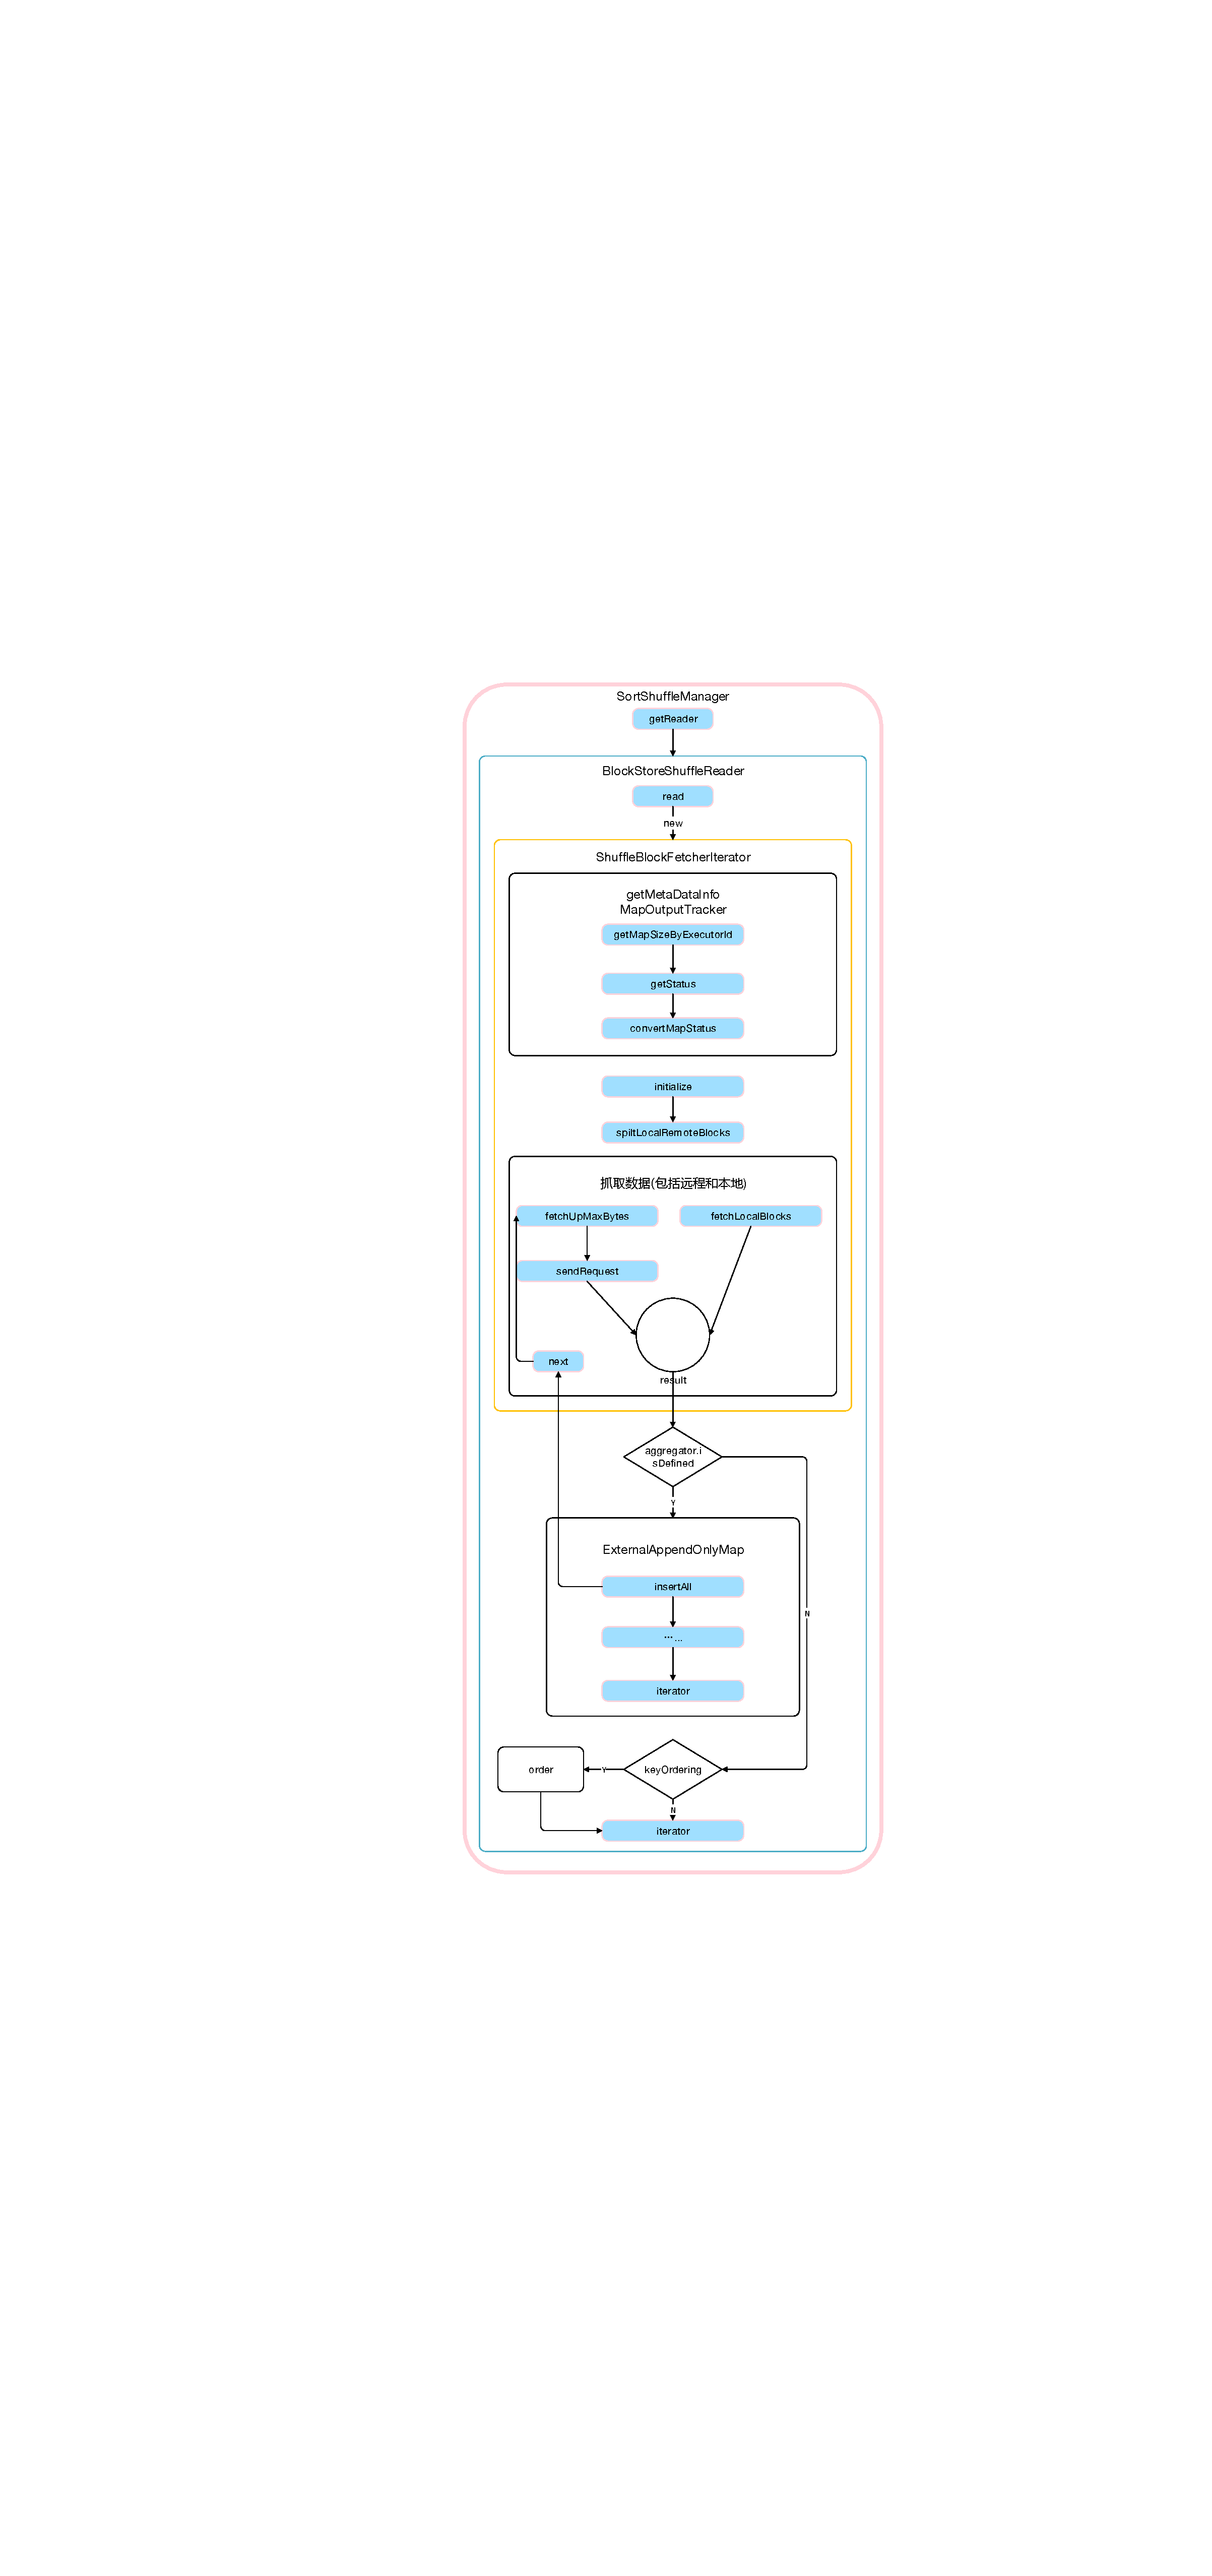
\includegraphics[width=0.85\textwidth,height=0.97\textheight]{figures/sortShuffleReadDia.pdf}
	\caption{shuffleread详细实现}
	\label{fig:shuffleread}
\end{figure}
\chapter{存储体系}
\section{概述}
块管理器BlockManager是Spark存储体系中的核心组件,其初始化在SparkEnv创建过程中,会首先创建BlockManagerMaster,之后再创建BlockManager,最后会在SparkContext中taskscheduler初始化完成后,调用\_env.blockManager.initialize(\_applicationId)完成初始化工作如程序\ref{inputPrg:creatBlockManager}所示
\begin{codeInput}{Scala}{BlockManager的初始化}{creatBlockManager}
//管理所有数据,无论在哪的数据,创建BlockManager
val blockManager = new BlockManager(executorId, rpcEnv, blockManagerMaster,serializer, conf, memoryManager, mapOutputTracker, shuffleManager,blockTransferService, securityManager, numUsableCores)
//blockTransferService的初始化和shuffleClient的初始化,shuffleClient默认是NettyBlockTransferService
blockTransferService.init(this)
shuffleClient.init(appId)
blockManagerId = BlockManagerId(
executorId, blockTransferService.hostName, blockTransferService.port)
//当有外部的ShuffleService时,创建新的BlockManagerId,否则就利用现有的blockManagerId
shuffleServerId = if (externalShuffleServiceEnabled) {
  BlockManagerId(executorId, blockTransferService.hostName, externalShuffleServicePort)
} else {
  blockManagerId
}
//向BlockManagerMaster注册blockManagerId slaveEndpoint
  master.registerBlockManager(blockManagerId, maxMemory, slaveEndpoint)
if (externalShuffleServiceEnabled && !blockManagerId.isDriver) {
  registerWithExternalShuffleServer()
}
\end{codeInput}

程序中在向BlockManagerMaster注册的时候会向判断当前进程是否为Driver。这是因为Driver和Executor中都会对SparkEnv进行初始化,且执行代码相同,

Spark存储体系架构图如\ref{fig:SparkArc}所示
\begin{figure}[H] 
	\centering
	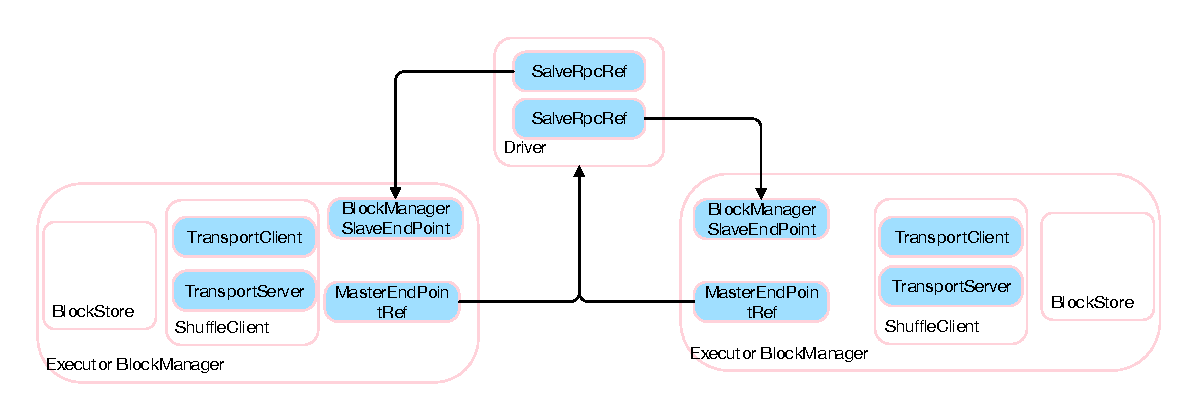
\includegraphics[width=\textwidth]{figures/storage.pdf}
	\caption{Spark存储体系架构}
	\label{fig:SparkArc}
\end{figure}

Spark定义了抽象类BlockStore,用于指定所有的存储类型规范。Spark1.6版本中定义了三种实现MemoryStore、DiskStore和ExternalBlockStore,其类图如图\ref{fig:BlockStore}所示
\begin{figure}[H] 
	\centering
	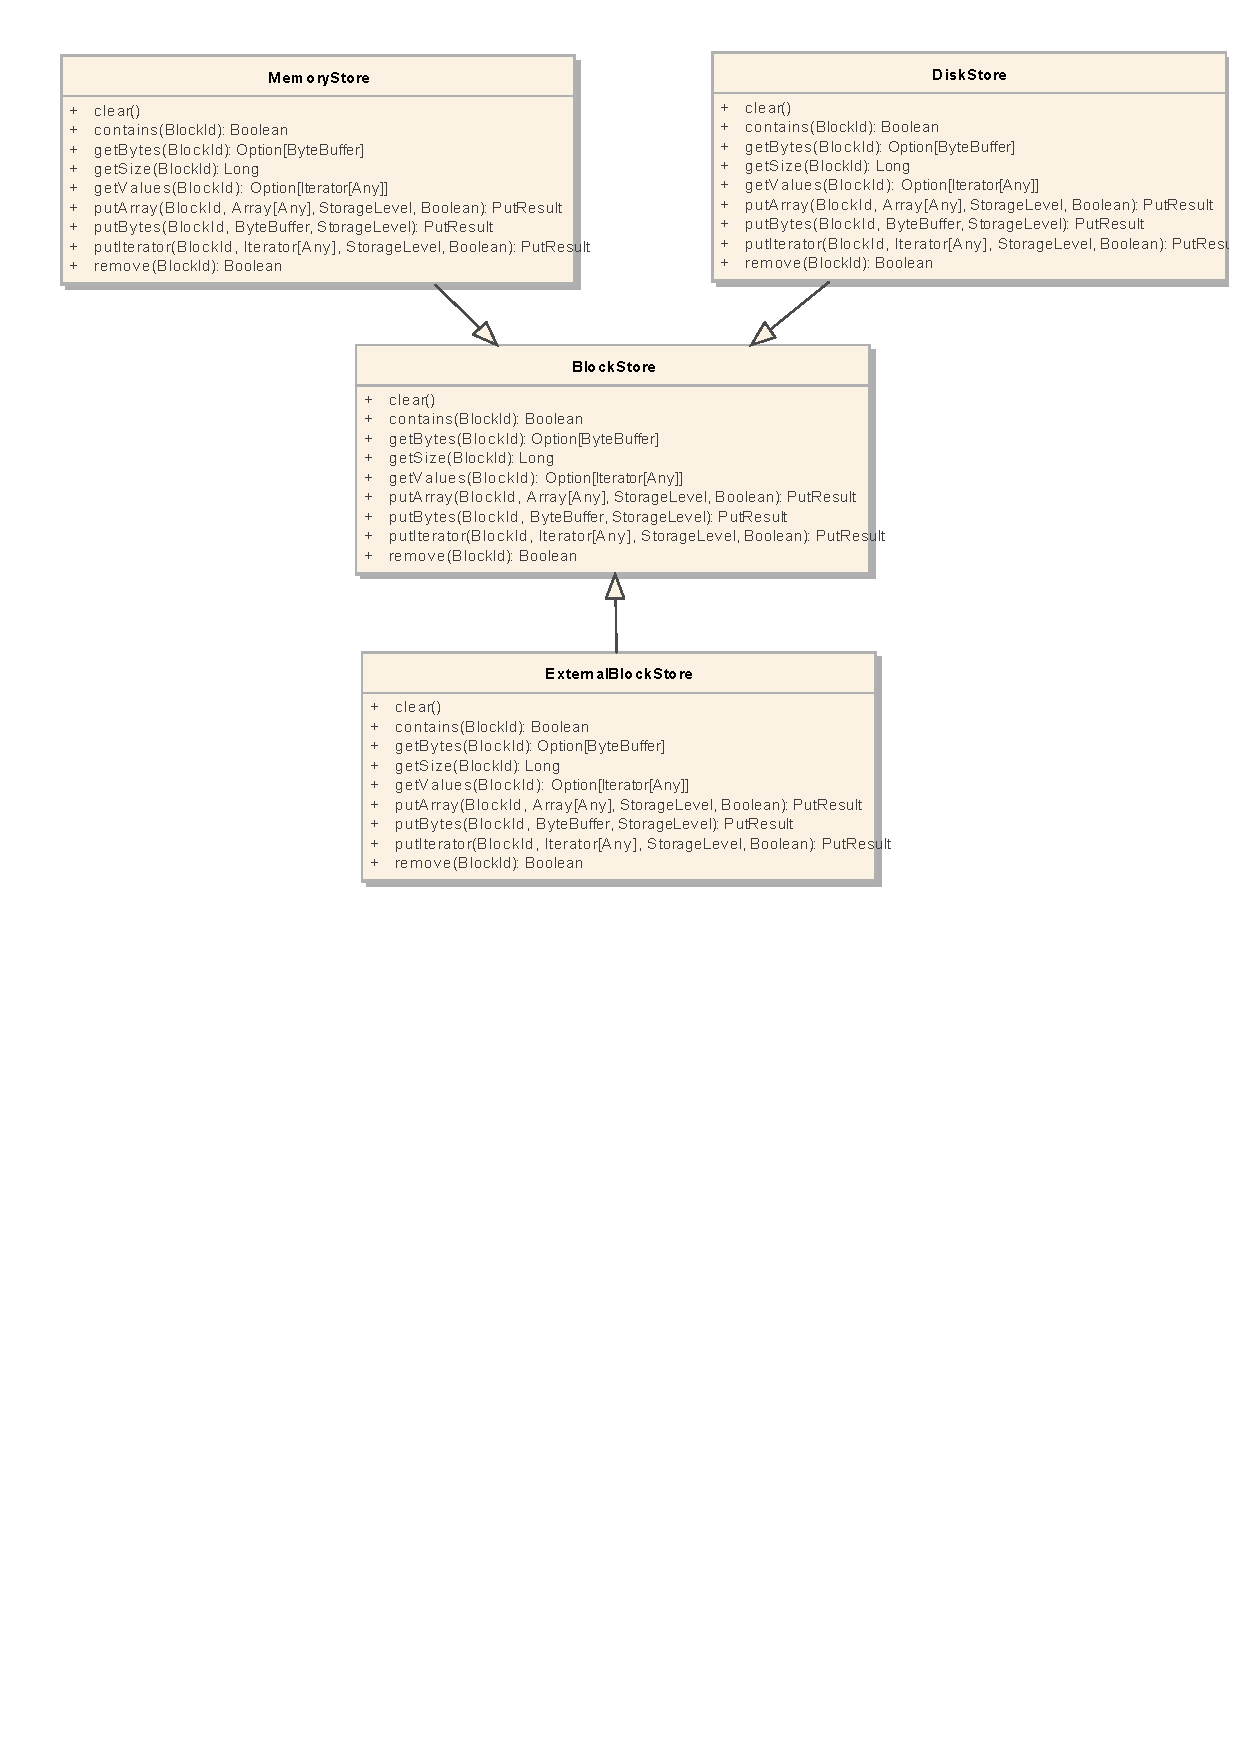
\includegraphics[width=\textwidth]{figures/BlockStore.pdf}
	\caption{BlockStore类图结构}
	\label{fig:BlockStore}
\end{figure}

\section{ShuffleClient模块}
由于Spark是分布式部署的,每个Task最终都运行在不同的机器节点上,map任务的输出结果直接存储在map任务所在的机器的存储体系中,reduce任务极有可能不在同一机器上运行,所以需要远程下载map任务的中间结果,这时存储体系中的ShuffleClient就可以发挥作用了。

ShuffleClient并不只是shuffle的客户端,它即包含了client,可以将shuffle文件上传到其他Executor或者从其他Executor下载文件到本地,同时也为其他Executor提供shuffle服务。在spark1.6中shuffleClient在没有开启externalShuffleService时即为NettyBlockTransferService。其初始化内容如程序\ref{inputPrg:nettyBlockTransferService}所示
\begin{codeInput}{Scala}{nettyBlockTransferService初始化}{nettyBlockTransferService}
override def init(blockDataManager: BlockDataManager): Unit = {
  //创建rpc服务
  val rpcHandler = new NettyBlockRpcServer(conf.getAppId, serializer, blockDataManager)
  var serverBootstrap: Option[TransportServerBootstrap] = None
  var clientBootstrap: Option[TransportClientBootstrap] = None
  if (authEnabled) {
    serverBootstrap = Some(new SaslServerBootstrap(transportConf, securityManager))
    clientBootstrap = Some(new SaslClientBootstrap(transportConf, conf.getAppId, securityManager,
    securityManager.isSaslEncryptionEnabled()))
  }
  //创建TransportContext
  transportContext = new TransportContext(transportConf, rpcHandler)
  //创建RPC客户端工厂
  clientFactory = transportContext.createClientFactory(clientBootstrap.toSeq.asJava)
  //创建Netty服务器TransportServer,端口由spark.blockManager.port控制
  server = createServer(serverBootstrap.toList)
  appId = conf.getAppId
}
\end{codeInput}

\subsection{Block的RPC服务}
在map和reduce两端,当reduce任务需要从远处节点Executor上下载map中间输出时,NettyBlockRpcServer需要提供下载Block文件的功能;同时,为了容错,也需要将Block的数据上传到其他节点,所以NettyBlockRpcServer还提供上传功能。NettyBlockRpcServer核心功能代码如程序\ref{inputPrg:NettyBlockRpcServer}
\begin{codeInput}{Scala}{NettyBlockRpcServer核心实现}{NettyBlockRpcServer}
message match {
  case openBlocks: OpenBlocks =>
    val blocks: Seq[ManagedBuffer]=openBlocks.blockIds.map(BlockId.apply).map(blockManager.getBlockData)
    val streamId = streamManager.registerStream(appId, blocks.iterator.asJava)
    logTrace(s"Registered streamId $streamId with ${blocks.size} buffers")
    responseContext.onSuccess(new StreamHandle(streamId, blocks.size).toByteBuffer)
  case uploadBlock: UploadBlock =>
    val level: StorageLevel =serializer.newInstance().deserialize(ByteBuffer.wrap(uploadBlock.metadata))
    val data = new NioManagedBuffer(ByteBuffer.wrap(uploadBlock.blockData))
    blockManager.putBlockData(BlockId(uploadBlock.blockId), data, level)
    responseContext.onSuccess(ByteBuffer.allocate(0))
\end{codeInput}
\subsection{传输上下文TransportContext}
TransportContext用Java编写,TransportContext既可以创建Netty服务,也可以创建Netty客户端。其构造器代码如程序\ref{inputPrg:TransportContext}所示
\begin{codeInput}{Java}{TransportContext构造器}{TransportContext}
public TransportContext(
TransportConf conf,
RpcHandler rpcHandler,
boolean closeIdleConnections) {
  //主要控制Netty框架提供的shuffle的I/O交互的客户端和服务器线程数量
  this.conf = conf;
  //负责shuffle的I/O服务端在接收到客户端RPC请求后,提供打开Block或者上传Block的RPC处理,此处即为NettyBlockRpcServer
  this.rpcHandler = rpcHandler;
  //在shuffle的I/O客户端对消息进行编码
  this.encoder = new MessageEncoder();
  //在shuffle的I/O服务端对客户端传来的ByteBuf进行解析,防止丢包和解析出错
  this.decoder = new MessageDecoder();
  this.closeIdleConnections = closeIdleConnections;
}
\end{codeInput}
\subsection{RPC客户端TransportClientFactory}
TransportClientFactory是创建Netty客户端TransporClient的工厂类,TransportClient用于向Netty服务端发送RPC请求。
TransportClientFactory主要部分如程序\ref{inputPrg:TransportClientFactory}所示
\begin{codeInput}{Java}{TransportClientFactory构造器}{TransportClientFactory}
public TransportClientFactory(
TransportContext context,
List<TransportClientBootstrap> clientBootstraps) {
  this.context = Preconditions.checkNotNull(context);
  this.conf = context.getConf();
  //缓存客户端列表
  this.clientBootstraps = Lists.newArrayList(Preconditions.checkNotNull(clientBootstraps));
  //缓存客户端连接
  this.connectionPool = new ConcurrentHashMap<SocketAddress, ClientPool>();
  //节点之间去数据的连接数,可以使用属性spark.shuffle.io.numConnectionsPerPeer来设置,默认为1
  this.numConnectionsPerPeer = conf.numConnectionsPerPeer();
  this.rand = new Random();	
  IOMode ioMode = IOMode.valueOf(conf.ioMode());
  //客户端channel被创建时使用的类,spark.shuffle.io.mode来配置,默认为NioSocketChannel
  this.socketChannelClass = NettyUtils.getClientChannelClass(ioMode);
  // TODO: Make thread pool name configurable.
  //根据Netty规范,客户端只有Work组,所以此处创建workerGroup,实际上是NioEventLoopGroup
  this.workerGroup = NettyUtils.createEventLoop(ioMode, conf.clientThreads(), "shuffle-client");
  //汇集ByteBuf但对本地线程缓存禁用的分配器
  this.pooledAllocator = NettyUtils.createPooledByteBufAllocator(
  conf.preferDirectBufs(), false /* allowCache */, conf.clientThreads());
}
\end{codeInput}
\subsection{Netty服务器TransportServer}
TransportServer提供了Netty实现的服务器端,用于提供RPC服务,上传、下载等。
\subsection{获取远程shuffle文件}
在上一节中可以看到在获取远程shuffle文件时调用的是shuffleClient.fetchBlocks,实际上是利用NettyBlockTransferService中创建Netty服务。具体的函数实现如程序\ref{inputPrg:shuffleFetchBlocks}所示
\begin{codeInput}{Scala}{获取远端节点上的shuffle文件}{shuffleFetchBlocks}
override def fetchBlocks(
host: String,
port: Int,
execId: String,
blockIds: Array[String],
listener: BlockFetchingListener): Unit = {
    val blockFetchStarter = new RetryingBlockFetcher.BlockFetchStarter {
      override def createAndStart(blockIds: Array[String], listener: BlockFetchingListener) {
        val client = clientFactory.createClient(host, port)
        new OneForOneBlockFetcher(client, appId, execId, blockIds.toArray, listener).start()
      }
    }
    val maxRetries = transportConf.maxIORetries()
    if (maxRetries > 0) {
      new RetryingBlockFetcher(transportConf, blockFetchStarter, blockIds, listener).start()
    } else {
      blockFetchStarter.createAndStart(blockIds, listener)
    }
}
\end{codeInput}
\subsection{上传shuffle文件}
NettyBlockTransferService的上传功能也是利用了NettyBlockTransferService中创建的Netty服务。具体实现如程序\ref{inputPrg:uploadBlock}所示
\begin{codeInput}{Scala}{uploadBlock实现}{uploadBlock}
override def uploadBlock(
hostname: String,
port: Int,
execId: String,
blockId: BlockId,
blockData: ManagedBuffer,
level: StorageLevel): Future[Unit] = {
  val result = Promise[Unit]()
  //创建Netty服务客户端
  val client = clientFactory.createClient(hostname, port)	
  //将Block的存储级别StorageLevel序列化
  val levelBytes = serializer.newInstance().serialize(level).array()
  //将Block中的ByteBuffer转化为数组,便于序列化	
  val nioBuffer = blockData.nioByteBuffer()	
  val array = if (nioBuffer.hasArray) {
    nioBuffer.array()
  } else {
    val data = new Array[Byte](nioBuffer.remaining())
    nioBuffer.get(data)
    data
  }
  //调用Netty客户端的snedRpc方法将字节数组上传,回调RpcResponseCallback
  client.sendRpc(new UploadBlock(appId, execId, blockId.toString, levelBytes, array).toByteBuffer,
    new RpcResponseCallback {
      override def onSuccess(response: ByteBuffer): Unit = {
        result.success((): Unit)
      }
      override def onFailure(e: Throwable): Unit = {
        result.failure(e)
      }
  })
  result.future
}
\end{codeInput}
\section{BlockManagerMaster对BlockManager的管理}
Driver上的BlockManagerMaster对存在于Executor上的BlockManager统一管理,比如Executor注册BlockManger、更新Executor上Block的最新信息。Spark作为分布式处理框架,在管理上是Driver端持有BlockManagerMasterEndpoint,所有的Executor上会有个BlockManagerMasterEndpointRef,所有的Executor与Driver在BlockManger的交互都依赖于它。
\subsection{BlockManagerMasterEndpoint}
BlockManagerMasterEndpoint只存在于Driver上,在Executor启动时会加载和Driver中一样的SparkEnv,这里会完成对Driver中BlockManagerMasterEndpoint的引用。然后通过其给BlockManagerMasterEndpoint发消息,实现与Driver的交互。
BlockManagerMasterEndpoint维护了很多缓存数据结构,重点看下面三个
\begin{enumerate}[\bfseries 1]
	\item blockManagerInfo
	
	其类型为HashMap[BlockManagerId, BlockManagerInfo],缓存所有的BlockManagerId及其BlockManager的信息
	\item blockManagerIdByExecutor
	
	其类型为HashMap[String, BlockManagerId],缓存executorId与其拥有的BlockManagerId之间的映射关系
	\item blockLocations
	
	其类型为JHashMap[BlockId, mutable.HashSet[BlockManagerId]],缓存Block与BlockManagerId直接的映射关系
\end{enumerate}
\subsection{BlockManagerSlaveEndpoint}
在每个Executor上都会运行一个BlockManagerSlaveEndpoint,用来接收Driver中BlockManagerMaster的消息。在Executor对BlockManager初始化时会调用BlockManagerMaster.registerBlockManager来向Dirver中的BlockManagerMaster注册BlockManger的信息,如程序\ref{inputPrg:registerBlockManager}所示
\begin{codeInput}{Scala}{registerBlockManager}{registerBlockManager}
def registerBlockManager(
blockManagerId: BlockManagerId, maxMemSize: Long, slaveEndpoint: RpcEndpointRef): Unit = {
  logInfo("Trying to register BlockManager")
  tell(RegisterBlockManager(blockManagerId, maxMemSize, slaveEndpoint))
  logInfo("Registered BlockManager")
}
\end{codeInput}

由上面的代码可以看出,Executor端会将blockManagerId、最大内存和BlockManagerSlaveEndpoint封装为RegisterBlockManager消息,通过Executor端持有的BlockManagerMasterEndpointRef向Driver端运行的BlockManagerMaster注册。Driver收到Executor注册的消息后会对传来的消息内容进行处理,具体的处理如程序\ref{inputPrg:driverRegisterBlockManager}所示,注册的时候会对blockManagerIdByExecutor和blockManagerInfo两个HashMap进行数据更新,此时Driver中的BlockManagerMaster就拥有了Executor中BlockManager的信息,且持有了对应的BlockManagerSlaveEndpointRef。
\begin{codeInput}{Scala}{Driver注册BlockManager实现}{driverRegisterBlockManager}
private def register(id: BlockManagerId, maxMemSize: Long, slaveEndpoint: RpcEndpointRef) {
  val time = System.currentTimeMillis()
  //确保blockManagerInfo持有消息中的BlockManagerId及其对应信息
  if (!blockManagerInfo.contains(id)) {
    //确保一个Executor只有一个BlockManagerId
    blockManagerIdByExecutor.get(id.executorId) match {
    //旧的BlockManagerId会被移除
      case Some(oldId) =>
        removeExecutor(id.executorId)
      case None =>
    }
  blockManagerIdByExecutor(id.executorId) = id	
  blockManagerInfo(id) = new BlockManagerInfo(id, System.currentTimeMillis(), maxMemSize, slaveEndpoint)
  }
  //最后向listenerBus推送一个SparkListenerBlockManagerAdded消息
  listenerBus.post(SparkListenerBlockManagerAdded(time, id, maxMemSize))
}
\end{codeInput}
\section{磁盘管理器DiskBlockManager}
磁盘管理器的创建在新建BlockManager实例的时候,它将在spark.local.dir中配置的目录下创建二级目录,二级目录的个数由spark.diskStore.subDirectories指定,默认为64.这些目录里面将会保存Block数据,新建二级目录用于对文件进行散列存储,散列存储可以是所有的文件都随机存放,写入或删除文件都很方便,存取速度快,节省时间。另外一个重要的方法就是getFile,程序要获取磁盘上的文件都是通过getFile进行的,其中subDirs是二维数组,用来缓存一级目录和二级目录。这里也使用了Spark磁盘散列文件存储的实现机制。如程序\ref{inputPrg:getFile}所示
\begin{codeInput}{Scala}{getFile的实现}{getFile}
def getFile(filename: String): File = {
  //根据文件名blockId.name计算哈希值
  val hash = Utils.nonNegativeHash(filename)
  //根据哈希值与本地文件一级目录的总数求余数,记为dirId
  val dirId = hash % localDirs.length
  //根据哈希值与本地文件一级目录的总数求商,此商与二级目录的数据在求余数,记为subDirId
  val subDirId = (hash / localDirs.length) % subDirsPerLocalDir	
  //如果dirId/subDirId目录存在,则获取dirId/subDirId目录下的文件
  val subDir = subDirs(dirId).synchronized {
    val old = subDirs(dirId)(subDirId)
    if (old != null) {
      old
    } else {
      //否则新建dirId/subDirId目录
      val newDir = new File(localDirs(dirId), "%02x".format(subDirId))
      if (!newDir.exists() && !newDir.mkdir()) {
        throw new IOException(s"Failed to create local dir in \$newDir.")
      }
      subDirs(dirId)(subDirId) = newDir
      newDir
    }
  }	
  new File(subDir, filename)
}
\end{codeInput}
\section{内存存储MemoryStore}
MemoryStore存储的是没有序列化的Java对象数组或者序列化的ByteBuffer存储到内存中,Spark中MemoryStore的内存模型如图\ref{fig:memoryStore}所示
\begin{figure}[H] 
	\centering
	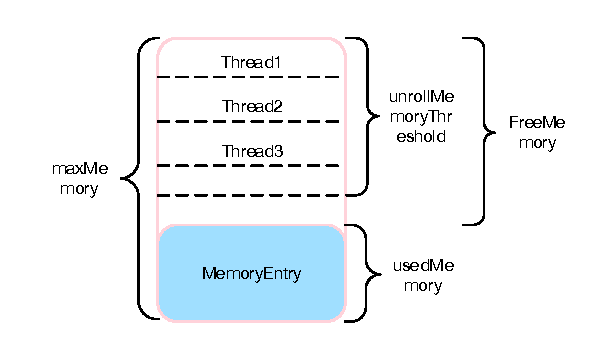
\includegraphics[width=\textwidth]{figures/memoryStore.pdf}
	\caption{MemoryStore的内存模型}
	\label{fig:memoryStore}
\end{figure}

如图\ref{fig:memoryStore}中看出,MemoryStore的存储可以分为两部分
\begin{enumerate}[\bfseries 1]
	\item MemoryEntry组成的usedMemory,这些Memory实际是通过entries持有的
	\item unrollMemoryMap被各线程提前预定,就像占座一样
\end{enumerate}
\section{磁盘存储DiskStore}
当MemoryStore没有足够空间时,就会使用DiskStore将块存入磁盘。
%%% 其它部分
%\backmatter

%% 本科生要这几个索引,研究生不要。选择性留下。
% 插图索引
%\listoffigures
% 表格索引
%\listoftables
% 公式索引
%\listofequations


%% 参考文献
% 注意:至少需要引用一篇参考文献,否则下面两行可能引起编译错误。
% 如果不需要参考文献,请将下面两行删除或注释掉。
%\bibliographystyle{thuthesis}
%\bibliography{ref/refs}


%% 致谢
%% 如果使用声明扫描页,将可选参数指定为扫描后的 PDF 文件名,例如:
% \begin{ack}[scan-statement.pdf]
\begin{acknowledgement}
  衷心感谢导师 xxx 教授和物理系 xxx 副教授对本人的精心指导。他们的言传身教将使
  我终生受益。

  在美国麻省理工学院化学系进行九个月的合作研究期间,承蒙 xxx 教授热心指导与帮助,不
  胜感激。感谢 xx 实验室主任 xx 教授,以及实验室全体老师和同学们的热情帮助和支
  持!本课题承蒙国家自然科学基金资助,特此致谢。

  感谢 \thuthesis,它的存在让我的论文写作轻松自在了许多,让我的论文格式规整漂亮了
  许多。
\end{acknowledgement}


%% 附录
%\begin{appendix}
%\chapter{外文资料原文}
\label{cha:engorg}

\title{The title of the English paper}

\textbf{Abstract:} As one of the most widely used techniques in operations
research, \emph{ mathematical programming} is defined as a means of maximizing a
quantity known as \emph{bjective function}, subject to a set of constraints
represented by equations and inequalities. Some known subtopics of mathematical
programming are linear programming, nonlinear programming, multiobjective
programming, goal programming, dynamic programming, and multilevel
programming$^{[1]}$.

It is impossible to cover in a single chapter every concept of mathematical
programming. This chapter introduces only the basic concepts and techniques of
mathematical programming such that readers gain an understanding of them
throughout the book$^{[2,3]}$.


\section{Single-Objective Programming}
The general form of single-objective programming (SOP) is written
as follows,
\begin{equation}\tag*{(123)} % 如果附录中的公式不想让它出现在公式索引中,那就请
                             % 用 \tag*{xxxx}
\left\{\begin{array}{l}
\max \,\,f(x)\\[0.1 cm]
\mbox{subject to:} \\ [0.1 cm]
\qquad g_j(x)\le 0,\quad j=1,2,\cdots,p
\end{array}\right.
\end{equation}
which maximizes a real-valued function $f$ of
$x=(x_1,x_2,\cdots,x_n)$ subject to a set of constraints.

\newtheorem{mpdef}{Definition}[chapter]
\begin{mpdef}
In SOP, we call $x$ a decision vector, and
$x_1,x_2,\cdots,x_n$ decision variables. The function
$f$ is called the objective function. The set
\begin{equation}\tag*{(456)} % 这里同理,其它不再一一指定。
S=\left\{x\in\Re^n\bigm|g_j(x)\le 0,\,j=1,2,\cdots,p\right\}
\end{equation}
is called the feasible set. An element $x$ in $S$ is called a
feasible solution.
\end{mpdef}

\newtheorem{mpdefop}[mpdef]{Definition}
\begin{mpdefop}
A feasible solution $x^*$ is called the optimal
solution of SOP if and only if
\begin{equation}
f(x^*)\ge f(x)
\end{equation}
for any feasible solution $x$.
\end{mpdefop}

One of the outstanding contributions to mathematical programming was known as
the Kuhn-Tucker conditions\ref{eq:ktc}. In order to introduce them, let us give
some definitions. An inequality constraint $g_j(x)\le 0$ is said to be active at
a point $x^*$ if $g_j(x^*)=0$. A point $x^*$ satisfying $g_j(x^*)\le 0$ is said
to be regular if the gradient vectors $\nabla g_j(x)$ of all active constraints
are linearly independent.

Let $x^*$ be a regular point of the constraints of SOP and assume that all the
functions $f(x)$ and $g_j(x),j=1,2,\cdots,p$ are differentiable. If $x^*$ is a
local optimal solution, then there exist Lagrange multipliers
$\lambda_j,j=1,2,\cdots,p$ such that the following Kuhn-Tucker conditions hold,
\begin{equation}
\label{eq:ktc}
\left\{\begin{array}{l}
    \nabla f(x^*)-\sum\limits_{j=1}^p\lambda_j\nabla g_j(x^*)=0\\[0.3cm]
    \lambda_jg_j(x^*)=0,\quad j=1,2,\cdots,p\\[0.2cm]
    \lambda_j\ge 0,\quad j=1,2,\cdots,p.
\end{array}\right.
\end{equation}
If all the functions $f(x)$ and $g_j(x),j=1,2,\cdots,p$ are convex and
differentiable, and the point $x^*$ satisfies the Kuhn-Tucker conditions
(\ref{eq:ktc}), then it has been proved that the point $x^*$ is a global optimal
solution of SOP.

\subsection{Linear Programming}
\label{sec:lp}

If the functions $f(x),g_j(x),j=1,2,\cdots,p$ are all linear, then SOP is called
a {\em linear programming}.

The feasible set of linear is always convex. A point $x$ is called an extreme
point of convex set $S$ if $x\in S$ and $x$ cannot be expressed as a convex
combination of two points in $S$. It has been shown that the optimal solution to
linear programming corresponds to an extreme point of its feasible set provided
that the feasible set $S$ is bounded. This fact is the basis of the {\em simplex
  algorithm} which was developed by Dantzig as a very efficient method for
solving linear programming.
\begin{table}[ht]
\centering
  \centering
  \caption*{Table~1\hskip1em This is an example for manually numbered table, which
    would not appear in the list of tables}
  \label{tab:badtabular2}
  \begin{tabular}[c]{|m{1.5cm}|c|c|c|c|c|c|}\hline
    \multicolumn{2}{|c|}{Network Topology} & \# of nodes &
    \multicolumn{3}{c|}{\# of clients} & Server \\\hline
    GT-ITM & Waxman Transit-Stub & 600 &
    \multirow{2}{2em}{2\%}&
    \multirow{2}{2em}{10\%}&
    \multirow{2}{2em}{50\%}&
    \multirow{2}{1.2in}{Max. Connectivity}\\\cline{1-3}
    \multicolumn{2}{|c|}{Inet-2.1} & 6000 & & & &\\\hline
    \multirow{2}{1.5cm}{Xue} & Rui  & Ni &\multicolumn{4}{c|}{\multirow{2}*{\thuthesis}}\\\cline{2-3}
    & \multicolumn{2}{c|}{ABCDEF} &\multicolumn{4}{c|}{} \\\hline
\end{tabular}
\end{table}

Roughly speaking, the simplex algorithm examines only the extreme points of the
feasible set, rather than all feasible points. At first, the simplex algorithm
selects an extreme point as the initial point. The successive extreme point is
selected so as to improve the objective function value. The procedure is
repeated until no improvement in objective function value can be made. The last
extreme point is the optimal solution.

\subsection{Nonlinear Programming}

If at least one of the functions $f(x),g_j(x),j=1,2,\cdots,p$ is nonlinear, then
SOP is called a {\em nonlinear programming}.

A large number of classical optimization methods have been developed to treat
special-structural nonlinear programming based on the mathematical theory
concerned with analyzing the structure of problems.
\begin{figure}[h]
  \centering
  
\includegraphics{thu-lib-logo}
  \caption*{Figure~1\quad This is an example for manually numbered figure,
    which would not appear in the list of figures}
  \label{tab:badfigure2}
\end{figure}

Now we consider a nonlinear programming which is confronted solely with
maximizing a real-valued function with domain $\Re^n$.  Whether derivatives are
available or not, the usual strategy is first to select a point in $\Re^n$ which
is thought to be the most likely place where the maximum exists. If there is no
information available on which to base such a selection, a point is chosen at
random. From this first point an attempt is made to construct a sequence of
points, each of which yields an improved objective function value over its
predecessor. The next point to be added to the sequence is chosen by analyzing
the behavior of the function at the previous points. This construction continues
until some termination criterion is met. Methods based upon this strategy are
called {\em ascent methods}, which can be classified as {\em direct methods},
{\em gradient methods}, and {\em Hessian methods} according to the information
about the behavior of objective function $f$. Direct methods require only that
the function can be evaluated at each point. Gradient methods require the
evaluation of first derivatives of $f$. Hessian methods require the evaluation
of second derivatives. In fact, there is no superior method for all
problems. The efficiency of a method is very much dependent upon the objective
function.

\subsection{Integer Programming}

{\em Integer programming} is a special mathematical programming in which all of
the variables are assumed to be only integer values. When there are not only
integer variables but also conventional continuous variables, we call it {\em
  mixed integer programming}. If all the variables are assumed either 0 or 1,
then the problem is termed a {\em zero-one programming}. Although integer
programming can be solved by an {\em exhaustive enumeration} theoretically, it
is impractical to solve realistically sized integer programming problems. The
most successful algorithm so far found to solve integer programming is called
the {\em branch-and-bound enumeration} developed by Balas (1965) and Dakin
(1965). The other technique to integer programming is the {\em cutting plane
  method} developed by Gomory (1959).

\hfill\textit{Uncertain Programming\/}\quad(\textsl{BaoDing Liu, 2006.2})

\section*{References}
\noindent{\itshape NOTE: These references are only for demonstration. They are
  not real citations in the original text.}

\begin{translationbib}
\item Donald E. Knuth. The \TeX book. Addison-Wesley, 1984. ISBN: 0-201-13448-9
\item Paul W. Abrahams, Karl Berry and Kathryn A. Hargreaves. \TeX\ for the
  Impatient. Addison-Wesley, 1990. ISBN: 0-201-51375-7
\item David Salomon. The advanced \TeX book.  New York : Springer, 1995. ISBN:0-387-94556-3
\end{translationbib}

\chapter{外文资料的调研阅读报告或书面翻译}

\title{英文资料的中文标题}

{\heiti 摘要:} 本章为外文资料翻译内容。如果有摘要可以直接写上来,这部分好像没有
明确的规定。

\section{单目标规划}
北冥有鱼,其名为鲲。鲲之大,不知其几千里也。化而为鸟,其名为鹏。鹏之背,不知其几
千里也。怒而飞,其翼若垂天之云。是鸟也,海运则将徙于南冥。南冥者,天池也。
\begin{equation}\tag*{(123)}
 p(y|\mathbf{x}) = \frac{p(\mathbf{x},y)}{p(\mathbf{x})}=
\frac{p(\mathbf{x}|y)p(y)}{p(\mathbf{x})}
\end{equation}

吾生也有涯,而知也无涯。以有涯随无涯,殆已!已而为知者,殆而已矣!为善无近名,为
恶无近刑,缘督以为经,可以保身,可以全生,可以养亲,可以尽年。

\subsection{线性规划}
庖丁为文惠君解牛,手之所触,肩之所倚,足之所履,膝之所倚,砉然响然,奏刀騞然,莫
不中音,合于桑林之舞,乃中经首之会。
\begin{table}[ht]
\centering
  \centering
  \caption*{表~1\hskip1em 这是手动编号但不出现在索引中的一个表格例子}
  \label{tab:badtabular3}
  \begin{tabular}[c]{|m{1.5cm}|c|c|c|c|c|c|}\hline
    \multicolumn{2}{|c|}{Network Topology} & \# of nodes &
    \multicolumn{3}{c|}{\# of clients} & Server \\\hline
    GT-ITM & Waxman Transit-Stub & 600 &
    \multirow{2}{2em}{2\%}&
    \multirow{2}{2em}{10\%}&
    \multirow{2}{2em}{50\%}&
    \multirow{2}{1.2in}{Max. Connectivity}\\\cline{1-3}
    \multicolumn{2}{|c|}{Inet-2.1} & 6000 & & & &\\\hline
    \multirow{2}{1.5cm}{Xue} & Rui  & Ni &\multicolumn{4}{c|}{\multirow{2}*{\thuthesis}}\\\cline{2-3}
    & \multicolumn{2}{c|}{ABCDEF} &\multicolumn{4}{c|}{} \\\hline
\end{tabular}
\end{table}

文惠君曰:“嘻,善哉!技盖至此乎?”庖丁释刀对曰:“臣之所好者道也,进乎技矣。始臣之
解牛之时,所见无非全牛者;三年之后,未尝见全牛也;方今之时,臣以神遇而不以目视,
官知止而神欲行。依乎天理,批大郤,导大窾,因其固然。技经肯綮之未尝,而况大坬乎!
良庖岁更刀,割也;族庖月更刀,折也;今臣之刀十九年矣,所解数千牛矣,而刀刃若新发
于硎。彼节者有间而刀刃者无厚,以无厚入有间,恢恢乎其于游刃必有余地矣。是以十九年
而刀刃若新发于硎。虽然,每至于族,吾见其难为,怵然为戒,视为止,行为迟,动刀甚微,
謋然已解,如土委地。提刀而立,为之而四顾,为之踌躇满志,善刀而藏之。”

文惠君曰:“善哉!吾闻庖丁之言,得养生焉。”


\subsection{非线性规划}
孔子与柳下季为友,柳下季之弟名曰盗跖。盗跖从卒九千人,横行天下,侵暴诸侯。穴室枢
户,驱人牛马,取人妇女。贪得忘亲,不顾父母兄弟,不祭先祖。所过之邑,大国守城,小
国入保,万民苦之。孔子谓柳下季曰:“夫为人父者,必能诏其子;为人兄者,必能教其弟。
若父不能诏其子,兄不能教其弟,则无贵父子兄弟之亲矣。今先生,世之才士也,弟为盗
跖,为天下害,而弗能教也,丘窃为先生羞之。丘请为先生往说之。”
\begin{figure}[h]
  \centering
  
\includegraphics{thu-whole-logo}
  \caption*{图~1\hskip1em 这是手动编号但不出现索引中的图片的例子}
  \label{tab:badfigure3}
\end{figure}

柳下季曰:“先生言为人父者必能诏其子,为人兄者必能教其弟,若子不听父之诏,弟不受
兄之教,虽今先生之辩,将奈之何哉?且跖之为人也,心如涌泉,意如飘风,强足以距敌,
辩足以饰非。顺其心则喜,逆其心则怒,易辱人以言。先生必无往。”

孔子不听,颜回为驭,子贡为右,往见盗跖。

\subsection{整数规划}
盗跖乃方休卒徒大山之阳,脍人肝而餔之。孔子下车而前,见谒者曰:“鲁人孔丘,闻将军
高义,敬再拜谒者。”谒者入通。盗跖闻之大怒,目如明星,发上指冠,曰:“此夫鲁国之
巧伪人孔丘非邪?为我告之:尔作言造语,妄称文、武,冠枝木之冠,带死牛之胁,多辞缪
说,不耕而食,不织而衣,摇唇鼓舌,擅生是非,以迷天下之主,使天下学士不反其本,妄
作孝弟,而侥幸于封侯富贵者也。子之罪大极重,疾走归!不然,我将以子肝益昼餔之膳。”


\chapter{其它附录}
前面两个附录主要是给本科生做例子。其它附录的内容可以放到这里,当然如果你愿意,可
以把这部分也放到独立的文件中,然后将其 \cs{input} 到主文件中。

%\end{appendix}

%% 个人简历
%\begin{resume}

  \resumeitem{个人简历}

  xxxx 年 xx 月 xx 日出生于 xx 省 xx 县。

  xxxx 年 9 月考入 xx 大学 xx 系 xx 专业,xxxx 年 7 月本科毕业并获得 xx 学士学位。

  xxxx 年 9 月免试进入 xx 大学 xx 系攻读 xx 学位至今。

  \researchitem{发表的学术论文} % 发表的和录用的合在一起

  % 1. 已经刊载的学术论文(本人是第一作者,或者导师为第一作者本人是第二作者)
  \begin{publications}
    \item Yang Y, Ren T L, Zhang L T, et al. Miniature microphone with silicon-
      based ferroelectric thin films. Integrated Ferroelectrics, 2003,
      52:229-235. (SCI 收录, 检索号:758FZ.)
    \item 杨轶, 张宁欣, 任天令, 等. 硅基铁电微声学器件中薄膜残余应力的研究. 中国机
      械工程, 2005, 16(14):1289-1291. (EI 收录, 检索号:0534931 2907.)
    \item 杨轶, 张宁欣, 任天令, 等. 集成铁电器件中的关键工艺研究. 仪器仪表学报,
      2003, 24(S4):192-193. (EI 源刊.)
  \end{publications}

  % 2. 尚未刊载,但已经接到正式录用函的学术论文(本人为第一作者,或者
  %    导师为第一作者本人是第二作者)。
  \begin{publications}[before=\publicationskip,after=\publicationskip]
    \item Yang Y, Ren T L, Zhu Y P, et al. PMUTs for handwriting recognition. In
      press. (已被 Integrated Ferroelectrics 录用. SCI 源刊.)
  \end{publications}

  % 3. 其他学术论文。可列出除上述两种情况以外的其他学术论文,但必须是
  %    已经刊载或者收到正式录用函的论文。
  \begin{publications}
    \item Wu X M, Yang Y, Cai J, et al. Measurements of ferroelectric MEMS
      microphones. Integrated Ferroelectrics, 2005, 69:417-429. (SCI 收录, 检索号
      :896KM)
    \item 贾泽, 杨轶, 陈兢, 等. 用于压电和电容微麦克风的体硅腐蚀相关研究. 压电与声
      光, 2006, 28(1):117-119. (EI 收录, 检索号:06129773469)
    \item 伍晓明, 杨轶, 张宁欣, 等. 基于MEMS技术的集成铁电硅微麦克风. 中国集成电路,
      2003, 53:59-61.
  \end{publications}

  \researchitem{研究成果} % 有就写,没有就删除
  \begin{achievements}
    \item 任天令, 杨轶, 朱一平, 等. 硅基铁电微声学传感器畴极化区域控制和电极连接的
      方法: 中国, CN1602118A. (中国专利公开号)
    \item Ren T L, Yang Y, Zhu Y P, et al. Piezoelectric micro acoustic sensor
      based on ferroelectric materials: USA, No.11/215, 102. (美国发明专利申请号)
  \end{achievements}

\end{resume}

\end{document}
